\documentclass[twoside]{book}

% Packages required by doxygen
\usepackage{fixltx2e}
\usepackage{calc}
\usepackage{doxygen}
\usepackage[export]{adjustbox} % also loads graphicx
\usepackage{graphicx}
\usepackage[utf8]{inputenc}
\usepackage{makeidx}
\usepackage{multicol}
\usepackage{multirow}
\PassOptionsToPackage{warn}{textcomp}
\usepackage{textcomp}
\usepackage[nointegrals]{wasysym}
\usepackage[table]{xcolor}

% Font selection
\usepackage[T1]{fontenc}
\usepackage[scaled=.90]{helvet}
\usepackage{courier}
\usepackage{amssymb}
\usepackage{sectsty}
\renewcommand{\familydefault}{\sfdefault}
\allsectionsfont{%
  \fontseries{bc}\selectfont%
  \color{darkgray}%
}
\renewcommand{\DoxyLabelFont}{%
  \fontseries{bc}\selectfont%
  \color{darkgray}%
}
\newcommand{\+}{\discretionary{\mbox{\scriptsize$\hookleftarrow$}}{}{}}

% Page & text layout
\usepackage{geometry}
\geometry{%
  a4paper,%
  top=2.5cm,%
  bottom=2.5cm,%
  left=2.5cm,%
  right=2.5cm%
}
\tolerance=750
\hfuzz=15pt
\hbadness=750
\setlength{\emergencystretch}{15pt}
\setlength{\parindent}{0cm}
\setlength{\parskip}{3ex plus 2ex minus 2ex}
\makeatletter
\renewcommand{\paragraph}{%
  \@startsection{paragraph}{4}{0ex}{-1.0ex}{1.0ex}{%
    \normalfont\normalsize\bfseries\SS@parafont%
  }%
}
\renewcommand{\subparagraph}{%
  \@startsection{subparagraph}{5}{0ex}{-1.0ex}{1.0ex}{%
    \normalfont\normalsize\bfseries\SS@subparafont%
  }%
}
\makeatother

% Headers & footers
\usepackage{fancyhdr}
\pagestyle{fancyplain}
\fancyhead[LE]{\fancyplain{}{\bfseries\thepage}}
\fancyhead[CE]{\fancyplain{}{}}
\fancyhead[RE]{\fancyplain{}{\bfseries\leftmark}}
\fancyhead[LO]{\fancyplain{}{\bfseries\rightmark}}
\fancyhead[CO]{\fancyplain{}{}}
\fancyhead[RO]{\fancyplain{}{\bfseries\thepage}}
\fancyfoot[LE]{\fancyplain{}{}}
\fancyfoot[CE]{\fancyplain{}{}}
\fancyfoot[RE]{\fancyplain{}{\bfseries\scriptsize Generated by Doxygen }}
\fancyfoot[LO]{\fancyplain{}{\bfseries\scriptsize Generated by Doxygen }}
\fancyfoot[CO]{\fancyplain{}{}}
\fancyfoot[RO]{\fancyplain{}{}}
\renewcommand{\footrulewidth}{0.4pt}
\renewcommand{\chaptermark}[1]{%
  \markboth{#1}{}%
}
\renewcommand{\sectionmark}[1]{%
  \markright{\thesection\ #1}%
}

% Indices & bibliography
\usepackage{natbib}
\usepackage[titles]{tocloft}
\setcounter{tocdepth}{3}
\setcounter{secnumdepth}{5}
\makeindex

% Hyperlinks (required, but should be loaded last)
\usepackage{ifpdf}
\ifpdf
  \usepackage[pdftex,pagebackref=true]{hyperref}
\else
  \usepackage[ps2pdf,pagebackref=true]{hyperref}
\fi
\hypersetup{%
  colorlinks=true,%
  linkcolor=blue,%
  citecolor=blue,%
  unicode%
}

% Custom commands
\newcommand{\clearemptydoublepage}{%
  \newpage{\pagestyle{empty}\cleardoublepage}%
}

\usepackage{caption}
\captionsetup{labelsep=space,justification=centering,font={bf},singlelinecheck=off,skip=4pt,position=top}

%===== C O N T E N T S =====

\begin{document}

% Titlepage & ToC
\hypersetup{pageanchor=false,
             bookmarksnumbered=true,
             pdfencoding=unicode
            }
\pagenumbering{alph}
\begin{titlepage}
\vspace*{7cm}
\begin{center}%
{\Large My Project }\\
\vspace*{1cm}
{\large Generated by Doxygen 1.8.13}\\
\end{center}
\end{titlepage}
\clearemptydoublepage
\pagenumbering{roman}
\tableofcontents
\clearemptydoublepage
\pagenumbering{arabic}
\hypersetup{pageanchor=true}

%--- Begin generated contents ---
\chapter{Data Structure Index}
\section{Data Structures}
Here are the data structures with brief descriptions\+:\begin{DoxyCompactList}
\item\contentsline{section}{\hyperlink{structBackground}{Background} }{\pageref{structBackground}}{}
\item\contentsline{section}{\hyperlink{structClochard}{Clochard} }{\pageref{structClochard}}{}
\item\contentsline{section}{\hyperlink{structhero}{hero} }{\pageref{structhero}}{}
\item\contentsline{section}{\hyperlink{structminimap}{minimap} }{\pageref{structminimap}}{}
\item\contentsline{section}{\hyperlink{structs__load}{s\+\_\+load} }{\pageref{structs__load}}{}
\item\contentsline{section}{\hyperlink{structs__menu}{s\+\_\+menu} }{\pageref{structs__menu}}{}
\item\contentsline{section}{\hyperlink{structScore}{Score} }{\pageref{structScore}}{}
\item\contentsline{section}{\hyperlink{structVie}{Vie} }{\pageref{structVie}}{}
\end{DoxyCompactList}

\chapter{File Index}
\section{File List}
Here is a list of all files with brief descriptions\+:\begin{DoxyCompactList}
\item\contentsline{section}{\hyperlink{amelioration__menu_8c}{amelioration\+\_\+menu.\+c} }{\pageref{amelioration__menu_8c}}{}
\item\contentsline{section}{\hyperlink{amelioration__menu_8h}{amelioration\+\_\+menu.\+h} \\*Ajout des touches }{\pageref{amelioration__menu_8h}}{}
\item\contentsline{section}{\hyperlink{background_8h}{background.\+h} }{\pageref{background_8h}}{}
\item\contentsline{section}{\hyperlink{bg_8c}{bg.\+c} }{\pageref{bg_8c}}{}
\item\contentsline{section}{\hyperlink{closhard_8c}{closhard.\+c} }{\pageref{closhard_8c}}{}
\item\contentsline{section}{\hyperlink{closhard_8h}{closhard.\+h} }{\pageref{closhard_8h}}{}
\item\contentsline{section}{\hyperlink{colis_8c}{colis.\+c} }{\pageref{colis_8c}}{}
\item\contentsline{section}{\hyperlink{colis_8h}{colis.\+h} }{\pageref{colis_8h}}{}
\item\contentsline{section}{\hyperlink{collision_8c}{collision.\+c} }{\pageref{collision_8c}}{}
\item\contentsline{section}{\hyperlink{collision_8h}{collision.\+h} }{\pageref{collision_8h}}{}
\item\contentsline{section}{\hyperlink{enigme3_8c}{enigme3.\+c} }{\pageref{enigme3_8c}}{}
\item\contentsline{section}{\hyperlink{enigme3_8h}{enigme3.\+h} }{\pageref{enigme3_8h}}{}
\item\contentsline{section}{\hyperlink{hero_8c}{hero.\+c} }{\pageref{hero_8c}}{}
\item\contentsline{section}{\hyperlink{hero_8h}{hero.\+h} }{\pageref{hero_8h}}{}
\item\contentsline{section}{\hyperlink{load_8c}{load.\+c} }{\pageref{load_8c}}{}
\item\contentsline{section}{\hyperlink{load_8h}{load.\+h} \\*Load }{\pageref{load_8h}}{}
\item\contentsline{section}{\hyperlink{lvl1_8c}{lvl1.\+c} }{\pageref{lvl1_8c}}{}
\item\contentsline{section}{\hyperlink{menu_8c}{menu.\+c} }{\pageref{menu_8c}}{}
\item\contentsline{section}{\hyperlink{menu_8h}{menu.\+h} }{\pageref{menu_8h}}{}
\item\contentsline{section}{\hyperlink{menu__jeu_8c}{menu\+\_\+jeu.\+c} }{\pageref{menu__jeu_8c}}{}
\item\contentsline{section}{\hyperlink{save_8c}{save.\+c} }{\pageref{save_8c}}{}
\item\contentsline{section}{\hyperlink{save_8h}{save.\+h} \\*Save }{\pageref{save_8h}}{}
\item\contentsline{section}{\hyperlink{score_8c}{score.\+c} }{\pageref{score_8c}}{}
\item\contentsline{section}{\hyperlink{score_8h}{score.\+h} }{\pageref{score_8h}}{}
\item\contentsline{section}{\hyperlink{scrolling_8c}{scrolling.\+c} }{\pageref{scrolling_8c}}{}
\item\contentsline{section}{\hyperlink{scrolling_8h}{scrolling.\+h} }{\pageref{scrolling_8h}}{}
\item\contentsline{section}{\hyperlink{t_8h}{t.\+h} }{\pageref{t_8h}}{}
\item\contentsline{section}{\hyperlink{temps_8c}{temps.\+c} }{\pageref{temps_8c}}{}
\item\contentsline{section}{\hyperlink{time_8c}{time.\+c} }{\pageref{time_8c}}{}
\item\contentsline{section}{\hyperlink{vie_8c}{vie.\+c} }{\pageref{vie_8c}}{}
\item\contentsline{section}{\hyperlink{vie_8h}{vie.\+h} }{\pageref{vie_8h}}{}
\end{DoxyCompactList}

\chapter{Data Structure Documentation}
\hypertarget{structBackground}{}\section{Background Struct Reference}
\label{structBackground}\index{Background@{Background}}


{\ttfamily \#include $<$background.\+h$>$}

\subsection*{Data Fields}
\begin{DoxyCompactItemize}
\item 
S\+D\+L\+\_\+\+Surface $\ast$ \hyperlink{structBackground_ac6c54173a0dc8a7e532abb15221ed6e8}{bg}
\item 
S\+D\+L\+\_\+\+Rect \hyperlink{structBackground_a364541c5bfd25f348775693cd3106f98}{position}
\item 
S\+D\+L\+\_\+\+Rect \hyperlink{structBackground_a1b6382669cea0e079a66ae195d09efd9}{scroll}
\item 
int \hyperlink{structBackground_a9ca8ab7528306796c4a254517458fdfe}{speed}
\item 
int \hyperlink{structBackground_a24bfe0184015610a8f9aacd98509d71b}{stage}
\end{DoxyCompactItemize}


\subsection{Field Documentation}
\mbox{\Hypertarget{structBackground_ac6c54173a0dc8a7e532abb15221ed6e8}\label{structBackground_ac6c54173a0dc8a7e532abb15221ed6e8}} 
\index{Background@{Background}!bg@{bg}}
\index{bg@{bg}!Background@{Background}}
\subsubsection{\texorpdfstring{bg}{bg}}
{\footnotesize\ttfamily S\+D\+L\+\_\+\+Surface$\ast$ Background\+::bg}

\mbox{\Hypertarget{structBackground_a364541c5bfd25f348775693cd3106f98}\label{structBackground_a364541c5bfd25f348775693cd3106f98}} 
\index{Background@{Background}!position@{position}}
\index{position@{position}!Background@{Background}}
\subsubsection{\texorpdfstring{position}{position}}
{\footnotesize\ttfamily S\+D\+L\+\_\+\+Rect Background\+::position}

\mbox{\Hypertarget{structBackground_a1b6382669cea0e079a66ae195d09efd9}\label{structBackground_a1b6382669cea0e079a66ae195d09efd9}} 
\index{Background@{Background}!scroll@{scroll}}
\index{scroll@{scroll}!Background@{Background}}
\subsubsection{\texorpdfstring{scroll}{scroll}}
{\footnotesize\ttfamily S\+D\+L\+\_\+\+Rect Background\+::scroll}

\mbox{\Hypertarget{structBackground_a9ca8ab7528306796c4a254517458fdfe}\label{structBackground_a9ca8ab7528306796c4a254517458fdfe}} 
\index{Background@{Background}!speed@{speed}}
\index{speed@{speed}!Background@{Background}}
\subsubsection{\texorpdfstring{speed}{speed}}
{\footnotesize\ttfamily int Background\+::speed}

\mbox{\Hypertarget{structBackground_a24bfe0184015610a8f9aacd98509d71b}\label{structBackground_a24bfe0184015610a8f9aacd98509d71b}} 
\index{Background@{Background}!stage@{stage}}
\index{stage@{stage}!Background@{Background}}
\subsubsection{\texorpdfstring{stage}{stage}}
{\footnotesize\ttfamily int Background\+::stage}



The documentation for this struct was generated from the following file\+:\begin{DoxyCompactItemize}
\item 
\hyperlink{background_8h}{background.\+h}\end{DoxyCompactItemize}

\hypertarget{structClochard}{}\section{Clochard Struct Reference}
\label{structClochard}\index{Clochard@{Clochard}}


{\ttfamily \#include $<$closhard.\+h$>$}

\subsection*{Data Fields}
\begin{DoxyCompactItemize}
\item 
S\+D\+L\+\_\+\+Surface $\ast$ \hyperlink{structClochard_a34522552cf1d2a44598bac76517e25ca}{sprite}
\item 
S\+D\+L\+\_\+\+Surface $\ast$ \hyperlink{structClochard_a1db48fc1cb139bdb2ccc18b675b59c60}{sprite2}
\item 
S\+D\+L\+\_\+\+Rect \hyperlink{structClochard_ac4bcafee4207a9233a3009916799d10c}{c\+\_\+pos}
\item 
int \hyperlink{structClochard_a1d43a4487cdf784496d9255a15f1c64e}{dx}
\item 
int \hyperlink{structClochard_a85da10470ca6863f61ca2e5734a2420f}{cx}
\end{DoxyCompactItemize}


\subsection{Field Documentation}
\mbox{\Hypertarget{structClochard_ac4bcafee4207a9233a3009916799d10c}\label{structClochard_ac4bcafee4207a9233a3009916799d10c}} 
\index{Clochard@{Clochard}!c\+\_\+pos@{c\+\_\+pos}}
\index{c\+\_\+pos@{c\+\_\+pos}!Clochard@{Clochard}}
\subsubsection{\texorpdfstring{c\+\_\+pos}{c\_pos}}
{\footnotesize\ttfamily S\+D\+L\+\_\+\+Rect Clochard\+::c\+\_\+pos}

\mbox{\Hypertarget{structClochard_a85da10470ca6863f61ca2e5734a2420f}\label{structClochard_a85da10470ca6863f61ca2e5734a2420f}} 
\index{Clochard@{Clochard}!cx@{cx}}
\index{cx@{cx}!Clochard@{Clochard}}
\subsubsection{\texorpdfstring{cx}{cx}}
{\footnotesize\ttfamily int Clochard\+::cx}

\mbox{\Hypertarget{structClochard_a1d43a4487cdf784496d9255a15f1c64e}\label{structClochard_a1d43a4487cdf784496d9255a15f1c64e}} 
\index{Clochard@{Clochard}!dx@{dx}}
\index{dx@{dx}!Clochard@{Clochard}}
\subsubsection{\texorpdfstring{dx}{dx}}
{\footnotesize\ttfamily int Clochard\+::dx}

\mbox{\Hypertarget{structClochard_a34522552cf1d2a44598bac76517e25ca}\label{structClochard_a34522552cf1d2a44598bac76517e25ca}} 
\index{Clochard@{Clochard}!sprite@{sprite}}
\index{sprite@{sprite}!Clochard@{Clochard}}
\subsubsection{\texorpdfstring{sprite}{sprite}}
{\footnotesize\ttfamily S\+D\+L\+\_\+\+Surface$\ast$ Clochard\+::sprite}

\mbox{\Hypertarget{structClochard_a1db48fc1cb139bdb2ccc18b675b59c60}\label{structClochard_a1db48fc1cb139bdb2ccc18b675b59c60}} 
\index{Clochard@{Clochard}!sprite2@{sprite2}}
\index{sprite2@{sprite2}!Clochard@{Clochard}}
\subsubsection{\texorpdfstring{sprite2}{sprite2}}
{\footnotesize\ttfamily S\+D\+L\+\_\+\+Surface $\ast$ Clochard\+::sprite2}



The documentation for this struct was generated from the following file\+:\begin{DoxyCompactItemize}
\item 
\hyperlink{closhard_8h}{closhard.\+h}\end{DoxyCompactItemize}

\hypertarget{structhero}{}\section{hero Struct Reference}
\label{structhero}\index{hero@{hero}}


{\ttfamily \#include $<$hero.\+h$>$}

\subsection*{Data Fields}
\begin{DoxyCompactItemize}
\item 
S\+D\+L\+\_\+\+Surface $\ast$ \hyperlink{structhero_a93cb673f8b54b6f7b365eb1fe22cbd91}{heroright}
\item 
S\+D\+L\+\_\+\+Surface $\ast$ \hyperlink{structhero_ac9349d1cfe5da7b8d52892f7eba3edb9}{heroleft}
\item 
S\+D\+L\+\_\+\+Rect \hyperlink{structhero_ac00c690d14ead4118a92d604f8885761}{positionhero}
\item 
S\+D\+L\+\_\+\+Rect \hyperlink{structhero_a5087f6cc23af7165275189406050fce5}{testt}
\item 
S\+D\+L\+\_\+\+Rect \hyperlink{structhero_a696a0a143c37c32c2cf037464a103f22}{rectright} \mbox{[}6\mbox{]}
\item 
S\+D\+L\+\_\+\+Rect \hyperlink{structhero_aac84e4428f223985f0c57f83ef7e5e56}{rectleft} \mbox{[}6\mbox{]}
\item 
int \hyperlink{structhero_aab107c0e79485d866f6903fdefe340bc}{directionhero}
\item 
int \hyperlink{structhero_a8affba68a94772ef439a2ee68b244ff8}{frame}
\item 
int \hyperlink{structhero_a913f57781151e585e18018cd8249d871}{g}
\begin{DoxyCompactList}\small\item\em J\+U\+MP. \end{DoxyCompactList}\item 
int \hyperlink{structhero_a42f83a5a147475aa2fa73a5ff07d2e89}{v}
\item 
int \hyperlink{structhero_ab02ce82098eb82b0c3be544f4624113f}{jump}
\end{DoxyCompactItemize}


\subsection{Field Documentation}
\mbox{\Hypertarget{structhero_aab107c0e79485d866f6903fdefe340bc}\label{structhero_aab107c0e79485d866f6903fdefe340bc}} 
\index{hero@{hero}!directionhero@{directionhero}}
\index{directionhero@{directionhero}!hero@{hero}}
\subsubsection{\texorpdfstring{directionhero}{directionhero}}
{\footnotesize\ttfamily int hero\+::directionhero}

\mbox{\Hypertarget{structhero_a8affba68a94772ef439a2ee68b244ff8}\label{structhero_a8affba68a94772ef439a2ee68b244ff8}} 
\index{hero@{hero}!frame@{frame}}
\index{frame@{frame}!hero@{hero}}
\subsubsection{\texorpdfstring{frame}{frame}}
{\footnotesize\ttfamily int hero\+::frame}

\mbox{\Hypertarget{structhero_a913f57781151e585e18018cd8249d871}\label{structhero_a913f57781151e585e18018cd8249d871}} 
\index{hero@{hero}!g@{g}}
\index{g@{g}!hero@{hero}}
\subsubsection{\texorpdfstring{g}{g}}
{\footnotesize\ttfamily int hero\+::g}



J\+U\+MP. 

\mbox{\Hypertarget{structhero_ac9349d1cfe5da7b8d52892f7eba3edb9}\label{structhero_ac9349d1cfe5da7b8d52892f7eba3edb9}} 
\index{hero@{hero}!heroleft@{heroleft}}
\index{heroleft@{heroleft}!hero@{hero}}
\subsubsection{\texorpdfstring{heroleft}{heroleft}}
{\footnotesize\ttfamily S\+D\+L\+\_\+\+Surface$\ast$ hero\+::heroleft}

\mbox{\Hypertarget{structhero_a93cb673f8b54b6f7b365eb1fe22cbd91}\label{structhero_a93cb673f8b54b6f7b365eb1fe22cbd91}} 
\index{hero@{hero}!heroright@{heroright}}
\index{heroright@{heroright}!hero@{hero}}
\subsubsection{\texorpdfstring{heroright}{heroright}}
{\footnotesize\ttfamily S\+D\+L\+\_\+\+Surface$\ast$ hero\+::heroright}

\mbox{\Hypertarget{structhero_ab02ce82098eb82b0c3be544f4624113f}\label{structhero_ab02ce82098eb82b0c3be544f4624113f}} 
\index{hero@{hero}!jump@{jump}}
\index{jump@{jump}!hero@{hero}}
\subsubsection{\texorpdfstring{jump}{jump}}
{\footnotesize\ttfamily int hero\+::jump}

\mbox{\Hypertarget{structhero_ac00c690d14ead4118a92d604f8885761}\label{structhero_ac00c690d14ead4118a92d604f8885761}} 
\index{hero@{hero}!positionhero@{positionhero}}
\index{positionhero@{positionhero}!hero@{hero}}
\subsubsection{\texorpdfstring{positionhero}{positionhero}}
{\footnotesize\ttfamily S\+D\+L\+\_\+\+Rect hero\+::positionhero}

\mbox{\Hypertarget{structhero_aac84e4428f223985f0c57f83ef7e5e56}\label{structhero_aac84e4428f223985f0c57f83ef7e5e56}} 
\index{hero@{hero}!rectleft@{rectleft}}
\index{rectleft@{rectleft}!hero@{hero}}
\subsubsection{\texorpdfstring{rectleft}{rectleft}}
{\footnotesize\ttfamily S\+D\+L\+\_\+\+Rect hero\+::rectleft\mbox{[}6\mbox{]}}

\mbox{\Hypertarget{structhero_a696a0a143c37c32c2cf037464a103f22}\label{structhero_a696a0a143c37c32c2cf037464a103f22}} 
\index{hero@{hero}!rectright@{rectright}}
\index{rectright@{rectright}!hero@{hero}}
\subsubsection{\texorpdfstring{rectright}{rectright}}
{\footnotesize\ttfamily S\+D\+L\+\_\+\+Rect hero\+::rectright\mbox{[}6\mbox{]}}

\mbox{\Hypertarget{structhero_a5087f6cc23af7165275189406050fce5}\label{structhero_a5087f6cc23af7165275189406050fce5}} 
\index{hero@{hero}!testt@{testt}}
\index{testt@{testt}!hero@{hero}}
\subsubsection{\texorpdfstring{testt}{testt}}
{\footnotesize\ttfamily S\+D\+L\+\_\+\+Rect hero\+::testt}

\mbox{\Hypertarget{structhero_a42f83a5a147475aa2fa73a5ff07d2e89}\label{structhero_a42f83a5a147475aa2fa73a5ff07d2e89}} 
\index{hero@{hero}!v@{v}}
\index{v@{v}!hero@{hero}}
\subsubsection{\texorpdfstring{v}{v}}
{\footnotesize\ttfamily int hero\+::v}



The documentation for this struct was generated from the following file\+:\begin{DoxyCompactItemize}
\item 
\hyperlink{hero_8h}{hero.\+h}\end{DoxyCompactItemize}

\hypertarget{structminimap}{}\section{minimap Struct Reference}
\label{structminimap}\index{minimap@{minimap}}


{\ttfamily \#include $<$hero.\+h$>$}

\subsection*{Data Fields}
\begin{DoxyCompactItemize}
\item 
S\+D\+L\+\_\+\+Surface $\ast$ \hyperlink{structminimap_a91f3511bf598b0975ad0cc6cef01e083}{minimap}
\item 
S\+D\+L\+\_\+\+Surface $\ast$ \hyperlink{structminimap_a65975b9ab10e99ac2975d3b124e1fd95}{miniheroright}
\item 
S\+D\+L\+\_\+\+Surface $\ast$ \hyperlink{structminimap_ad2ac04771114b30c06cd0b6769da3adc}{miniheroleft}
\item 
S\+D\+L\+\_\+\+Surface $\ast$ \hyperlink{structminimap_ae4646d13e408c328abb6ba01678ff430}{arrow}
\item 
S\+D\+L\+\_\+\+Rect \hyperlink{structminimap_a5b8800e04dc9b89c2964d04c46a34da4}{positionminihero}
\item 
S\+D\+L\+\_\+\+Rect \hyperlink{structminimap_a1daef1078e2acbafbf95d9b37471847f}{positionminimap}
\item 
S\+D\+L\+\_\+\+Rect \hyperlink{structminimap_afdc2c993b098b8b208bde4b0195039c3}{positionarrow}
\end{DoxyCompactItemize}


\subsection{Field Documentation}
\mbox{\Hypertarget{structminimap_ae4646d13e408c328abb6ba01678ff430}\label{structminimap_ae4646d13e408c328abb6ba01678ff430}} 
\index{minimap@{minimap}!arrow@{arrow}}
\index{arrow@{arrow}!minimap@{minimap}}
\subsubsection{\texorpdfstring{arrow}{arrow}}
{\footnotesize\ttfamily S\+D\+L\+\_\+\+Surface $\ast$ minimap\+::arrow}

\mbox{\Hypertarget{structminimap_ad2ac04771114b30c06cd0b6769da3adc}\label{structminimap_ad2ac04771114b30c06cd0b6769da3adc}} 
\index{minimap@{minimap}!miniheroleft@{miniheroleft}}
\index{miniheroleft@{miniheroleft}!minimap@{minimap}}
\subsubsection{\texorpdfstring{miniheroleft}{miniheroleft}}
{\footnotesize\ttfamily S\+D\+L\+\_\+\+Surface $\ast$ minimap\+::miniheroleft}

\mbox{\Hypertarget{structminimap_a65975b9ab10e99ac2975d3b124e1fd95}\label{structminimap_a65975b9ab10e99ac2975d3b124e1fd95}} 
\index{minimap@{minimap}!miniheroright@{miniheroright}}
\index{miniheroright@{miniheroright}!minimap@{minimap}}
\subsubsection{\texorpdfstring{miniheroright}{miniheroright}}
{\footnotesize\ttfamily S\+D\+L\+\_\+\+Surface $\ast$ minimap\+::miniheroright}

\mbox{\Hypertarget{structminimap_a91f3511bf598b0975ad0cc6cef01e083}\label{structminimap_a91f3511bf598b0975ad0cc6cef01e083}} 
\index{minimap@{minimap}!minimap@{minimap}}
\index{minimap@{minimap}!minimap@{minimap}}
\subsubsection{\texorpdfstring{minimap}{minimap}}
{\footnotesize\ttfamily S\+D\+L\+\_\+\+Surface$\ast$ minimap\+::minimap}

\mbox{\Hypertarget{structminimap_afdc2c993b098b8b208bde4b0195039c3}\label{structminimap_afdc2c993b098b8b208bde4b0195039c3}} 
\index{minimap@{minimap}!positionarrow@{positionarrow}}
\index{positionarrow@{positionarrow}!minimap@{minimap}}
\subsubsection{\texorpdfstring{positionarrow}{positionarrow}}
{\footnotesize\ttfamily S\+D\+L\+\_\+\+Rect minimap\+::positionarrow}

\mbox{\Hypertarget{structminimap_a5b8800e04dc9b89c2964d04c46a34da4}\label{structminimap_a5b8800e04dc9b89c2964d04c46a34da4}} 
\index{minimap@{minimap}!positionminihero@{positionminihero}}
\index{positionminihero@{positionminihero}!minimap@{minimap}}
\subsubsection{\texorpdfstring{positionminihero}{positionminihero}}
{\footnotesize\ttfamily S\+D\+L\+\_\+\+Rect minimap\+::positionminihero}

\mbox{\Hypertarget{structminimap_a1daef1078e2acbafbf95d9b37471847f}\label{structminimap_a1daef1078e2acbafbf95d9b37471847f}} 
\index{minimap@{minimap}!positionminimap@{positionminimap}}
\index{positionminimap@{positionminimap}!minimap@{minimap}}
\subsubsection{\texorpdfstring{positionminimap}{positionminimap}}
{\footnotesize\ttfamily S\+D\+L\+\_\+\+Rect minimap\+::positionminimap}



The documentation for this struct was generated from the following file\+:\begin{DoxyCompactItemize}
\item 
\hyperlink{hero_8h}{hero.\+h}\end{DoxyCompactItemize}

\hypertarget{structs__load}{}\section{s\+\_\+load Struct Reference}
\label{structs__load}\index{s\+\_\+load@{s\+\_\+load}}


{\ttfamily \#include $<$load.\+h$>$}

\subsection*{Data Fields}
\begin{DoxyCompactItemize}
\item 
S\+D\+L\+\_\+\+Surface $\ast$ \hyperlink{structs__load_ae3f8bf434529b68a3773d90354040c3d}{menu}
\item 
S\+D\+L\+\_\+\+Surface $\ast$ \hyperlink{structs__load_a9ba58ada741b7d909ab635fe47a3e93d}{new1}
\item 
S\+D\+L\+\_\+\+Surface $\ast$ \hyperlink{structs__load_ab0e0c6d78418c4932183a397e28025ad}{load1}
\item 
S\+D\+L\+\_\+\+Rect \hyperlink{structs__load_ab8c7a36251dcdaf992072eccfbd7c868}{pos\+\_\+smenu}
\item 
S\+D\+L\+\_\+\+Rect \hyperlink{structs__load_a9cc546d0039e147179f72ebbefb89a49}{pos\+\_\+new}
\item 
S\+D\+L\+\_\+\+Rect \hyperlink{structs__load_ae94ceaa48f5d724e15d96ccee46b30f5}{pos\+\_\+load}
\end{DoxyCompactItemize}


\subsection{Field Documentation}
\mbox{\Hypertarget{structs__load_ab0e0c6d78418c4932183a397e28025ad}\label{structs__load_ab0e0c6d78418c4932183a397e28025ad}} 
\index{s\+\_\+load@{s\+\_\+load}!load1@{load1}}
\index{load1@{load1}!s\+\_\+load@{s\+\_\+load}}
\subsubsection{\texorpdfstring{load1}{load1}}
{\footnotesize\ttfamily S\+D\+L\+\_\+\+Surface $\ast$ s\+\_\+load\+::load1}

\mbox{\Hypertarget{structs__load_ae3f8bf434529b68a3773d90354040c3d}\label{structs__load_ae3f8bf434529b68a3773d90354040c3d}} 
\index{s\+\_\+load@{s\+\_\+load}!menu@{menu}}
\index{menu@{menu}!s\+\_\+load@{s\+\_\+load}}
\subsubsection{\texorpdfstring{menu}{menu}}
{\footnotesize\ttfamily S\+D\+L\+\_\+\+Surface$\ast$ s\+\_\+load\+::menu}

\mbox{\Hypertarget{structs__load_a9ba58ada741b7d909ab635fe47a3e93d}\label{structs__load_a9ba58ada741b7d909ab635fe47a3e93d}} 
\index{s\+\_\+load@{s\+\_\+load}!new1@{new1}}
\index{new1@{new1}!s\+\_\+load@{s\+\_\+load}}
\subsubsection{\texorpdfstring{new1}{new1}}
{\footnotesize\ttfamily S\+D\+L\+\_\+\+Surface $\ast$ s\+\_\+load\+::new1}

\mbox{\Hypertarget{structs__load_ae94ceaa48f5d724e15d96ccee46b30f5}\label{structs__load_ae94ceaa48f5d724e15d96ccee46b30f5}} 
\index{s\+\_\+load@{s\+\_\+load}!pos\+\_\+load@{pos\+\_\+load}}
\index{pos\+\_\+load@{pos\+\_\+load}!s\+\_\+load@{s\+\_\+load}}
\subsubsection{\texorpdfstring{pos\+\_\+load}{pos\_load}}
{\footnotesize\ttfamily S\+D\+L\+\_\+\+Rect s\+\_\+load\+::pos\+\_\+load}

\mbox{\Hypertarget{structs__load_a9cc546d0039e147179f72ebbefb89a49}\label{structs__load_a9cc546d0039e147179f72ebbefb89a49}} 
\index{s\+\_\+load@{s\+\_\+load}!pos\+\_\+new@{pos\+\_\+new}}
\index{pos\+\_\+new@{pos\+\_\+new}!s\+\_\+load@{s\+\_\+load}}
\subsubsection{\texorpdfstring{pos\+\_\+new}{pos\_new}}
{\footnotesize\ttfamily S\+D\+L\+\_\+\+Rect s\+\_\+load\+::pos\+\_\+new}

\mbox{\Hypertarget{structs__load_ab8c7a36251dcdaf992072eccfbd7c868}\label{structs__load_ab8c7a36251dcdaf992072eccfbd7c868}} 
\index{s\+\_\+load@{s\+\_\+load}!pos\+\_\+smenu@{pos\+\_\+smenu}}
\index{pos\+\_\+smenu@{pos\+\_\+smenu}!s\+\_\+load@{s\+\_\+load}}
\subsubsection{\texorpdfstring{pos\+\_\+smenu}{pos\_smenu}}
{\footnotesize\ttfamily S\+D\+L\+\_\+\+Rect s\+\_\+load\+::pos\+\_\+smenu}



The documentation for this struct was generated from the following file\+:\begin{DoxyCompactItemize}
\item 
\hyperlink{load_8h}{load.\+h}\end{DoxyCompactItemize}

\hypertarget{structs__menu}{}\section{s\+\_\+menu Struct Reference}
\label{structs__menu}\index{s\+\_\+menu@{s\+\_\+menu}}


{\ttfamily \#include $<$save.\+h$>$}

\subsection*{Data Fields}
\begin{DoxyCompactItemize}
\item 
S\+D\+L\+\_\+\+Surface $\ast$ \hyperlink{structs__menu_a63a54d0a1800992c818a7035e4b6cdfb}{menu}
\item 
S\+D\+L\+\_\+\+Surface $\ast$ \hyperlink{structs__menu_ae2cc359de85d9186f41239090425aa2e}{yes}
\item 
S\+D\+L\+\_\+\+Surface $\ast$ \hyperlink{structs__menu_a6a98a2b24b32b41da278e6db0a2e0bf0}{no}
\item 
S\+D\+L\+\_\+\+Rect \hyperlink{structs__menu_a94c480395e7615eea72ac573b49e2f05}{pos\+\_\+smenu}
\item 
S\+D\+L\+\_\+\+Rect \hyperlink{structs__menu_a885acf2f224092c5bf18906d461c7086}{pos\+\_\+yes}
\item 
S\+D\+L\+\_\+\+Rect \hyperlink{structs__menu_a843a16fd3756989eb7ceaaa3367ef995}{pos\+\_\+no}
\end{DoxyCompactItemize}


\subsection{Field Documentation}
\mbox{\Hypertarget{structs__menu_a63a54d0a1800992c818a7035e4b6cdfb}\label{structs__menu_a63a54d0a1800992c818a7035e4b6cdfb}} 
\index{s\+\_\+menu@{s\+\_\+menu}!menu@{menu}}
\index{menu@{menu}!s\+\_\+menu@{s\+\_\+menu}}
\subsubsection{\texorpdfstring{menu}{menu}}
{\footnotesize\ttfamily S\+D\+L\+\_\+\+Surface$\ast$ s\+\_\+menu\+::menu}

\mbox{\Hypertarget{structs__menu_a6a98a2b24b32b41da278e6db0a2e0bf0}\label{structs__menu_a6a98a2b24b32b41da278e6db0a2e0bf0}} 
\index{s\+\_\+menu@{s\+\_\+menu}!no@{no}}
\index{no@{no}!s\+\_\+menu@{s\+\_\+menu}}
\subsubsection{\texorpdfstring{no}{no}}
{\footnotesize\ttfamily S\+D\+L\+\_\+\+Surface $\ast$ s\+\_\+menu\+::no}

\mbox{\Hypertarget{structs__menu_a843a16fd3756989eb7ceaaa3367ef995}\label{structs__menu_a843a16fd3756989eb7ceaaa3367ef995}} 
\index{s\+\_\+menu@{s\+\_\+menu}!pos\+\_\+no@{pos\+\_\+no}}
\index{pos\+\_\+no@{pos\+\_\+no}!s\+\_\+menu@{s\+\_\+menu}}
\subsubsection{\texorpdfstring{pos\+\_\+no}{pos\_no}}
{\footnotesize\ttfamily S\+D\+L\+\_\+\+Rect s\+\_\+menu\+::pos\+\_\+no}

\mbox{\Hypertarget{structs__menu_a94c480395e7615eea72ac573b49e2f05}\label{structs__menu_a94c480395e7615eea72ac573b49e2f05}} 
\index{s\+\_\+menu@{s\+\_\+menu}!pos\+\_\+smenu@{pos\+\_\+smenu}}
\index{pos\+\_\+smenu@{pos\+\_\+smenu}!s\+\_\+menu@{s\+\_\+menu}}
\subsubsection{\texorpdfstring{pos\+\_\+smenu}{pos\_smenu}}
{\footnotesize\ttfamily S\+D\+L\+\_\+\+Rect s\+\_\+menu\+::pos\+\_\+smenu}

\mbox{\Hypertarget{structs__menu_a885acf2f224092c5bf18906d461c7086}\label{structs__menu_a885acf2f224092c5bf18906d461c7086}} 
\index{s\+\_\+menu@{s\+\_\+menu}!pos\+\_\+yes@{pos\+\_\+yes}}
\index{pos\+\_\+yes@{pos\+\_\+yes}!s\+\_\+menu@{s\+\_\+menu}}
\subsubsection{\texorpdfstring{pos\+\_\+yes}{pos\_yes}}
{\footnotesize\ttfamily S\+D\+L\+\_\+\+Rect s\+\_\+menu\+::pos\+\_\+yes}

\mbox{\Hypertarget{structs__menu_ae2cc359de85d9186f41239090425aa2e}\label{structs__menu_ae2cc359de85d9186f41239090425aa2e}} 
\index{s\+\_\+menu@{s\+\_\+menu}!yes@{yes}}
\index{yes@{yes}!s\+\_\+menu@{s\+\_\+menu}}
\subsubsection{\texorpdfstring{yes}{yes}}
{\footnotesize\ttfamily S\+D\+L\+\_\+\+Surface $\ast$ s\+\_\+menu\+::yes}



The documentation for this struct was generated from the following file\+:\begin{DoxyCompactItemize}
\item 
\hyperlink{save_8h}{save.\+h}\end{DoxyCompactItemize}

\hypertarget{structScore}{}\section{Score Struct Reference}
\label{structScore}\index{Score@{Score}}


{\ttfamily \#include $<$score.\+h$>$}

\subsection*{Data Fields}
\begin{DoxyCompactItemize}
\item 
S\+D\+L\+\_\+\+Surface $\ast$ \hyperlink{structScore_aea0f2011fc97c3a7776635a84b76fe67}{fond\+Score}
\item 
S\+D\+L\+\_\+\+Rect \hyperlink{structScore_a578e743bcee6d68e53de231fd0f0dbbf}{pos\+Fond}
\item 
S\+D\+L\+\_\+\+Surface $\ast$ \hyperlink{structScore_ae9a968b720621f536298fd15749463e2}{texte\+Score}
\item 
T\+T\+F\+\_\+\+Font $\ast$ \hyperlink{structScore_a7887e4dd262c08a37b568f3aa5ad30e2}{police}
\item 
S\+D\+L\+\_\+\+Rect \hyperlink{structScore_a163319fdcee50a9d6ff99dad49809ae9}{pos\+Score}
\item 
int \hyperlink{structScore_a1dc9e9448e13b692f49293078e2db059}{score\+Actuel}
\end{DoxyCompactItemize}


\subsection{Field Documentation}
\mbox{\Hypertarget{structScore_aea0f2011fc97c3a7776635a84b76fe67}\label{structScore_aea0f2011fc97c3a7776635a84b76fe67}} 
\index{Score@{Score}!fond\+Score@{fond\+Score}}
\index{fond\+Score@{fond\+Score}!Score@{Score}}
\subsubsection{\texorpdfstring{fond\+Score}{fondScore}}
{\footnotesize\ttfamily S\+D\+L\+\_\+\+Surface$\ast$ Score\+::fond\+Score}

\mbox{\Hypertarget{structScore_a7887e4dd262c08a37b568f3aa5ad30e2}\label{structScore_a7887e4dd262c08a37b568f3aa5ad30e2}} 
\index{Score@{Score}!police@{police}}
\index{police@{police}!Score@{Score}}
\subsubsection{\texorpdfstring{police}{police}}
{\footnotesize\ttfamily T\+T\+F\+\_\+\+Font$\ast$ Score\+::police}

\mbox{\Hypertarget{structScore_a578e743bcee6d68e53de231fd0f0dbbf}\label{structScore_a578e743bcee6d68e53de231fd0f0dbbf}} 
\index{Score@{Score}!pos\+Fond@{pos\+Fond}}
\index{pos\+Fond@{pos\+Fond}!Score@{Score}}
\subsubsection{\texorpdfstring{pos\+Fond}{posFond}}
{\footnotesize\ttfamily S\+D\+L\+\_\+\+Rect Score\+::pos\+Fond}

\mbox{\Hypertarget{structScore_a163319fdcee50a9d6ff99dad49809ae9}\label{structScore_a163319fdcee50a9d6ff99dad49809ae9}} 
\index{Score@{Score}!pos\+Score@{pos\+Score}}
\index{pos\+Score@{pos\+Score}!Score@{Score}}
\subsubsection{\texorpdfstring{pos\+Score}{posScore}}
{\footnotesize\ttfamily S\+D\+L\+\_\+\+Rect Score\+::pos\+Score}

\mbox{\Hypertarget{structScore_a1dc9e9448e13b692f49293078e2db059}\label{structScore_a1dc9e9448e13b692f49293078e2db059}} 
\index{Score@{Score}!score\+Actuel@{score\+Actuel}}
\index{score\+Actuel@{score\+Actuel}!Score@{Score}}
\subsubsection{\texorpdfstring{score\+Actuel}{scoreActuel}}
{\footnotesize\ttfamily int Score\+::score\+Actuel}

\mbox{\Hypertarget{structScore_ae9a968b720621f536298fd15749463e2}\label{structScore_ae9a968b720621f536298fd15749463e2}} 
\index{Score@{Score}!texte\+Score@{texte\+Score}}
\index{texte\+Score@{texte\+Score}!Score@{Score}}
\subsubsection{\texorpdfstring{texte\+Score}{texteScore}}
{\footnotesize\ttfamily S\+D\+L\+\_\+\+Surface$\ast$ Score\+::texte\+Score}



The documentation for this struct was generated from the following file\+:\begin{DoxyCompactItemize}
\item 
\hyperlink{score_8h}{score.\+h}\end{DoxyCompactItemize}

\hypertarget{structVie}{}\section{Vie Struct Reference}
\label{structVie}\index{Vie@{Vie}}


{\ttfamily \#include $<$vie.\+h$>$}

\subsection*{Data Fields}
\begin{DoxyCompactItemize}
\item 
S\+D\+L\+\_\+\+Surface $\ast$ \hyperlink{structVie_ab737dfbd09f4f094fee7e7182c2610f6}{vie\+\_\+img1}
\item 
S\+D\+L\+\_\+\+Surface $\ast$ \hyperlink{structVie_aaf9de52d2a9ecce1d95b3caaf0f1c144}{vie\+\_\+img2}
\item 
S\+D\+L\+\_\+\+Surface $\ast$ \hyperlink{structVie_a0e8a93a5738e5b1f6a1b4e847f6e039d}{vie\+\_\+img3}
\item 
S\+D\+L\+\_\+\+Surface $\ast$ \hyperlink{structVie_a03c03529f7221ba0e219e440fd44ca68}{vie\+\_\+img4}
\item 
S\+D\+L\+\_\+\+Rect \hyperlink{structVie_aac5227324a8cc878e4e2c3b128a12856}{pos\+Vie}
\item 
int \hyperlink{structVie_a108db214817c1a00c67457b644569671}{val\+Vie}
\end{DoxyCompactItemize}


\subsection{Field Documentation}
\mbox{\Hypertarget{structVie_aac5227324a8cc878e4e2c3b128a12856}\label{structVie_aac5227324a8cc878e4e2c3b128a12856}} 
\index{Vie@{Vie}!pos\+Vie@{pos\+Vie}}
\index{pos\+Vie@{pos\+Vie}!Vie@{Vie}}
\subsubsection{\texorpdfstring{pos\+Vie}{posVie}}
{\footnotesize\ttfamily S\+D\+L\+\_\+\+Rect Vie\+::pos\+Vie}

\mbox{\Hypertarget{structVie_a108db214817c1a00c67457b644569671}\label{structVie_a108db214817c1a00c67457b644569671}} 
\index{Vie@{Vie}!val\+Vie@{val\+Vie}}
\index{val\+Vie@{val\+Vie}!Vie@{Vie}}
\subsubsection{\texorpdfstring{val\+Vie}{valVie}}
{\footnotesize\ttfamily int Vie\+::val\+Vie}

\mbox{\Hypertarget{structVie_ab737dfbd09f4f094fee7e7182c2610f6}\label{structVie_ab737dfbd09f4f094fee7e7182c2610f6}} 
\index{Vie@{Vie}!vie\+\_\+img1@{vie\+\_\+img1}}
\index{vie\+\_\+img1@{vie\+\_\+img1}!Vie@{Vie}}
\subsubsection{\texorpdfstring{vie\+\_\+img1}{vie\_img1}}
{\footnotesize\ttfamily S\+D\+L\+\_\+\+Surface$\ast$ Vie\+::vie\+\_\+img1}

\mbox{\Hypertarget{structVie_aaf9de52d2a9ecce1d95b3caaf0f1c144}\label{structVie_aaf9de52d2a9ecce1d95b3caaf0f1c144}} 
\index{Vie@{Vie}!vie\+\_\+img2@{vie\+\_\+img2}}
\index{vie\+\_\+img2@{vie\+\_\+img2}!Vie@{Vie}}
\subsubsection{\texorpdfstring{vie\+\_\+img2}{vie\_img2}}
{\footnotesize\ttfamily S\+D\+L\+\_\+\+Surface$\ast$ Vie\+::vie\+\_\+img2}

\mbox{\Hypertarget{structVie_a0e8a93a5738e5b1f6a1b4e847f6e039d}\label{structVie_a0e8a93a5738e5b1f6a1b4e847f6e039d}} 
\index{Vie@{Vie}!vie\+\_\+img3@{vie\+\_\+img3}}
\index{vie\+\_\+img3@{vie\+\_\+img3}!Vie@{Vie}}
\subsubsection{\texorpdfstring{vie\+\_\+img3}{vie\_img3}}
{\footnotesize\ttfamily S\+D\+L\+\_\+\+Surface$\ast$ Vie\+::vie\+\_\+img3}

\mbox{\Hypertarget{structVie_a03c03529f7221ba0e219e440fd44ca68}\label{structVie_a03c03529f7221ba0e219e440fd44ca68}} 
\index{Vie@{Vie}!vie\+\_\+img4@{vie\+\_\+img4}}
\index{vie\+\_\+img4@{vie\+\_\+img4}!Vie@{Vie}}
\subsubsection{\texorpdfstring{vie\+\_\+img4}{vie\_img4}}
{\footnotesize\ttfamily S\+D\+L\+\_\+\+Surface$\ast$ Vie\+::vie\+\_\+img4}



The documentation for this struct was generated from the following file\+:\begin{DoxyCompactItemize}
\item 
\hyperlink{vie_8h}{vie.\+h}\end{DoxyCompactItemize}

\chapter{File Documentation}
\hypertarget{amelioration__menu_8c}{}\section{amelioration\+\_\+menu.\+c File Reference}
\label{amelioration__menu_8c}\index{amelioration\+\_\+menu.\+c@{amelioration\+\_\+menu.\+c}}
{\ttfamily \#include $<$stdlib.\+h$>$}\newline
{\ttfamily \#include $<$stdio.\+h$>$}\newline
{\ttfamily \#include $<$S\+D\+L/\+S\+D\+L\+\_\+mixer.\+h$>$}\newline
{\ttfamily \#include $<$S\+D\+L/\+S\+D\+L\+\_\+image.\+h$>$}\newline
{\ttfamily \#include $<$S\+D\+L/\+S\+D\+L\+\_\+ttf.\+h$>$}\newline
{\ttfamily \#include $<$S\+D\+L/\+S\+D\+L.\+h$>$}\newline
{\ttfamily \#include \char`\"{}amelioration\+\_\+menu.\+h\char`\"{}}\newline
Include dependency graph for amelioration\+\_\+menu.\+c\+:\nopagebreak
\begin{figure}[H]
\begin{center}
\leavevmode
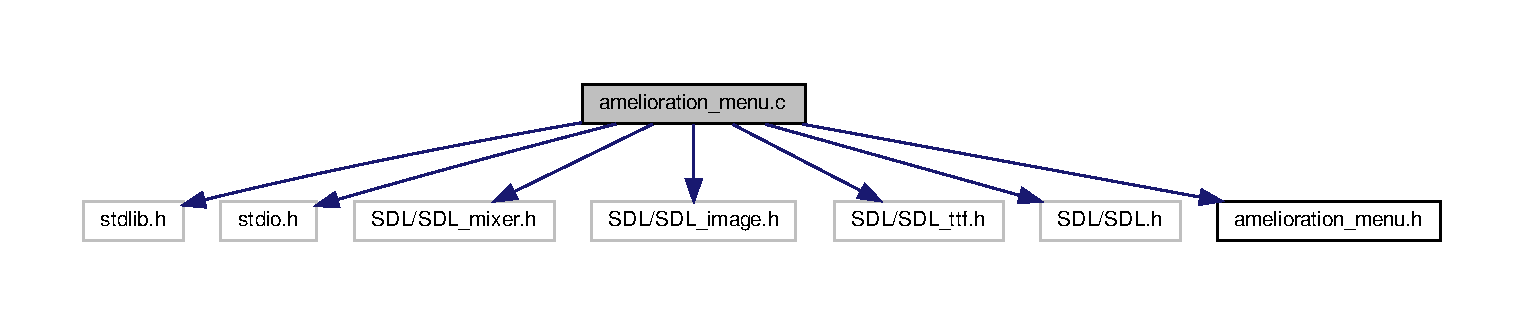
\includegraphics[width=350pt]{amelioration__menu_8c__incl}
\end{center}
\end{figure}
\subsection*{Functions}
\begin{DoxyCompactItemize}
\item 
int \hyperlink{amelioration__menu_8c_a1e0d526d92db41be5f0c1609a1071e61}{personnage} (S\+D\+L\+\_\+\+Surface $\ast$screen)
\item 
int \hyperlink{amelioration__menu_8c_a05ce82049441a0d5cf28ba1450108a61}{outil} (S\+D\+L\+\_\+\+Surface $\ast$screen)
\end{DoxyCompactItemize}


\subsection{Function Documentation}
\mbox{\Hypertarget{amelioration__menu_8c_a05ce82049441a0d5cf28ba1450108a61}\label{amelioration__menu_8c_a05ce82049441a0d5cf28ba1450108a61}} 
\index{amelioration\+\_\+menu.\+c@{amelioration\+\_\+menu.\+c}!outil@{outil}}
\index{outil@{outil}!amelioration\+\_\+menu.\+c@{amelioration\+\_\+menu.\+c}}
\subsubsection{\texorpdfstring{outil()}{outil()}}
{\footnotesize\ttfamily int outil (\begin{DoxyParamCaption}\item[{S\+D\+L\+\_\+\+Surface $\ast$}]{screen }\end{DoxyParamCaption})}

Here is the call graph for this function\+:\nopagebreak
\begin{figure}[H]
\begin{center}
\leavevmode
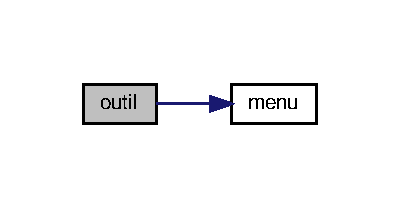
\includegraphics[width=192pt]{amelioration__menu_8c_a05ce82049441a0d5cf28ba1450108a61_cgraph}
\end{center}
\end{figure}
Here is the caller graph for this function\+:\nopagebreak
\begin{figure}[H]
\begin{center}
\leavevmode
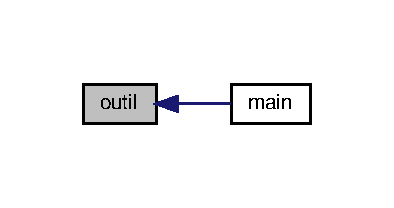
\includegraphics[width=189pt]{amelioration__menu_8c_a05ce82049441a0d5cf28ba1450108a61_icgraph}
\end{center}
\end{figure}
\mbox{\Hypertarget{amelioration__menu_8c_a1e0d526d92db41be5f0c1609a1071e61}\label{amelioration__menu_8c_a1e0d526d92db41be5f0c1609a1071e61}} 
\index{amelioration\+\_\+menu.\+c@{amelioration\+\_\+menu.\+c}!personnage@{personnage}}
\index{personnage@{personnage}!amelioration\+\_\+menu.\+c@{amelioration\+\_\+menu.\+c}}
\subsubsection{\texorpdfstring{personnage()}{personnage()}}
{\footnotesize\ttfamily int personnage (\begin{DoxyParamCaption}\item[{S\+D\+L\+\_\+\+Surface $\ast$}]{screen }\end{DoxyParamCaption})}

Here is the caller graph for this function\+:\nopagebreak
\begin{figure}[H]
\begin{center}
\leavevmode
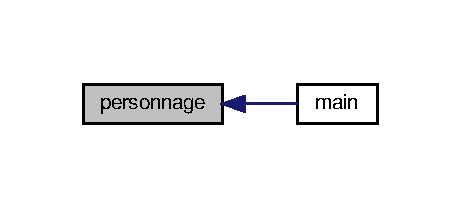
\includegraphics[width=221pt]{amelioration__menu_8c_a1e0d526d92db41be5f0c1609a1071e61_icgraph}
\end{center}
\end{figure}

\hypertarget{amelioration__menu_8h}{}\section{amelioration\+\_\+menu.\+h File Reference}
\label{amelioration__menu_8h}\index{amelioration\+\_\+menu.\+h@{amelioration\+\_\+menu.\+h}}


ajout des touches  


This graph shows which files directly or indirectly include this file\+:\nopagebreak
\begin{figure}[H]
\begin{center}
\leavevmode
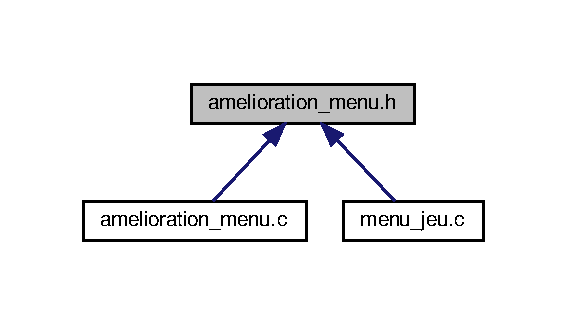
\includegraphics[width=272pt]{amelioration__menu_8h__dep__incl}
\end{center}
\end{figure}
\subsection*{Functions}
\begin{DoxyCompactItemize}
\item 
int \hyperlink{amelioration__menu_8h_a1e0d526d92db41be5f0c1609a1071e61}{personnage} (S\+D\+L\+\_\+\+Surface $\ast$screen)
\item 
int \hyperlink{amelioration__menu_8h_a05ce82049441a0d5cf28ba1450108a61}{outil} (S\+D\+L\+\_\+\+Surface $\ast$screen)
\end{DoxyCompactItemize}


\subsection{Detailed Description}
ajout des touches 

\begin{DoxyAuthor}{Author}
meriam mhedhbi 
\end{DoxyAuthor}


\subsection{Function Documentation}
\mbox{\Hypertarget{amelioration__menu_8h_a05ce82049441a0d5cf28ba1450108a61}\label{amelioration__menu_8h_a05ce82049441a0d5cf28ba1450108a61}} 
\index{amelioration\+\_\+menu.\+h@{amelioration\+\_\+menu.\+h}!outil@{outil}}
\index{outil@{outil}!amelioration\+\_\+menu.\+h@{amelioration\+\_\+menu.\+h}}
\subsubsection{\texorpdfstring{outil()}{outil()}}
{\footnotesize\ttfamily int outil (\begin{DoxyParamCaption}\item[{S\+D\+L\+\_\+\+Surface $\ast$}]{screen }\end{DoxyParamCaption})}

Here is the call graph for this function\+:\nopagebreak
\begin{figure}[H]
\begin{center}
\leavevmode
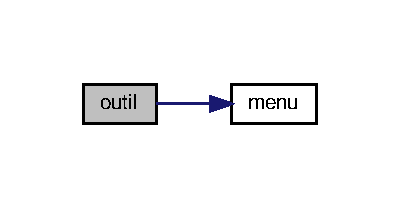
\includegraphics[width=192pt]{amelioration__menu_8h_a05ce82049441a0d5cf28ba1450108a61_cgraph}
\end{center}
\end{figure}
Here is the caller graph for this function\+:\nopagebreak
\begin{figure}[H]
\begin{center}
\leavevmode
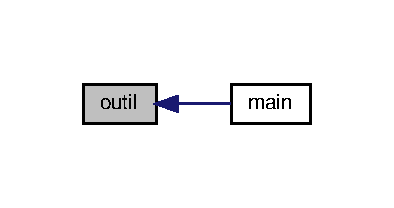
\includegraphics[width=189pt]{amelioration__menu_8h_a05ce82049441a0d5cf28ba1450108a61_icgraph}
\end{center}
\end{figure}
\mbox{\Hypertarget{amelioration__menu_8h_a1e0d526d92db41be5f0c1609a1071e61}\label{amelioration__menu_8h_a1e0d526d92db41be5f0c1609a1071e61}} 
\index{amelioration\+\_\+menu.\+h@{amelioration\+\_\+menu.\+h}!personnage@{personnage}}
\index{personnage@{personnage}!amelioration\+\_\+menu.\+h@{amelioration\+\_\+menu.\+h}}
\subsubsection{\texorpdfstring{personnage()}{personnage()}}
{\footnotesize\ttfamily int personnage (\begin{DoxyParamCaption}\item[{S\+D\+L\+\_\+\+Surface $\ast$}]{screen }\end{DoxyParamCaption})}

Here is the caller graph for this function\+:\nopagebreak
\begin{figure}[H]
\begin{center}
\leavevmode
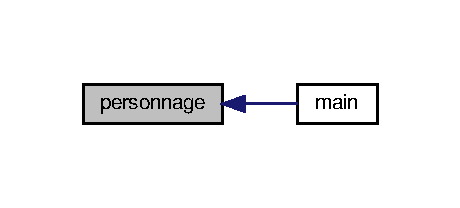
\includegraphics[width=221pt]{amelioration__menu_8h_a1e0d526d92db41be5f0c1609a1071e61_icgraph}
\end{center}
\end{figure}

\hypertarget{background_8h}{}\section{background.\+h File Reference}
\label{background_8h}\index{background.\+h@{background.\+h}}
This graph shows which files directly or indirectly include this file\+:\nopagebreak
\begin{figure}[H]
\begin{center}
\leavevmode
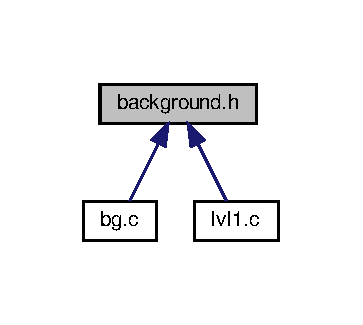
\includegraphics[width=174pt]{background_8h__dep__incl}
\end{center}
\end{figure}
\subsection*{Data Structures}
\begin{DoxyCompactItemize}
\item 
struct \hyperlink{structBackground}{Background}
\end{DoxyCompactItemize}
\subsection*{Macros}
\begin{DoxyCompactItemize}
\item 
\#define \hyperlink{background_8h_a9782776f04bdbb5674b628e683646f39}{B\+A\+C\+K\+G\+R\+O\+U\+N\+G\+\_\+\+H\+\_\+\+I\+N\+C\+L\+U\+D\+ED}
\end{DoxyCompactItemize}
\subsection*{Functions}
\begin{DoxyCompactItemize}
\item 
void \hyperlink{background_8h_a64ee95bd1a66087c4ffed437aaa4d550}{init\+\_\+bk} (\hyperlink{structBackground}{Background} $\ast$b)
\item 
void \hyperlink{background_8h_ae1687dac9508505654b9106ce8450282}{afficher\+\_\+bk} (\hyperlink{structBackground}{Background} $\ast$bk, S\+D\+L\+\_\+\+Surface $\ast$fenetre)
\item 
void \hyperlink{background_8h_a2e14fb88a1bcd685693bb2678f8b50b0}{scrollingbg} (\hyperlink{structBackground}{Background} $\ast$bg, S\+D\+L\+\_\+\+Surface $\ast$mario, S\+D\+L\+\_\+\+Rect mario\+\_\+position)
\end{DoxyCompactItemize}


\subsection{Macro Definition Documentation}
\mbox{\Hypertarget{background_8h_a9782776f04bdbb5674b628e683646f39}\label{background_8h_a9782776f04bdbb5674b628e683646f39}} 
\index{background.\+h@{background.\+h}!B\+A\+C\+K\+G\+R\+O\+U\+N\+G\+\_\+\+H\+\_\+\+I\+N\+C\+L\+U\+D\+ED@{B\+A\+C\+K\+G\+R\+O\+U\+N\+G\+\_\+\+H\+\_\+\+I\+N\+C\+L\+U\+D\+ED}}
\index{B\+A\+C\+K\+G\+R\+O\+U\+N\+G\+\_\+\+H\+\_\+\+I\+N\+C\+L\+U\+D\+ED@{B\+A\+C\+K\+G\+R\+O\+U\+N\+G\+\_\+\+H\+\_\+\+I\+N\+C\+L\+U\+D\+ED}!background.\+h@{background.\+h}}
\subsubsection{\texorpdfstring{B\+A\+C\+K\+G\+R\+O\+U\+N\+G\+\_\+\+H\+\_\+\+I\+N\+C\+L\+U\+D\+ED}{BACKGROUNG\_H\_INCLUDED}}
{\footnotesize\ttfamily \#define B\+A\+C\+K\+G\+R\+O\+U\+N\+G\+\_\+\+H\+\_\+\+I\+N\+C\+L\+U\+D\+ED}



\subsection{Function Documentation}
\mbox{\Hypertarget{background_8h_ae1687dac9508505654b9106ce8450282}\label{background_8h_ae1687dac9508505654b9106ce8450282}} 
\index{background.\+h@{background.\+h}!afficher\+\_\+bk@{afficher\+\_\+bk}}
\index{afficher\+\_\+bk@{afficher\+\_\+bk}!background.\+h@{background.\+h}}
\subsubsection{\texorpdfstring{afficher\+\_\+bk()}{afficher\_bk()}}
{\footnotesize\ttfamily void afficher\+\_\+bk (\begin{DoxyParamCaption}\item[{\hyperlink{structBackground}{Background} $\ast$}]{bk,  }\item[{S\+D\+L\+\_\+\+Surface $\ast$}]{fenetre }\end{DoxyParamCaption})}

\mbox{\Hypertarget{background_8h_a64ee95bd1a66087c4ffed437aaa4d550}\label{background_8h_a64ee95bd1a66087c4ffed437aaa4d550}} 
\index{background.\+h@{background.\+h}!init\+\_\+bk@{init\+\_\+bk}}
\index{init\+\_\+bk@{init\+\_\+bk}!background.\+h@{background.\+h}}
\subsubsection{\texorpdfstring{init\+\_\+bk()}{init\_bk()}}
{\footnotesize\ttfamily void init\+\_\+bk (\begin{DoxyParamCaption}\item[{\hyperlink{structBackground}{Background} $\ast$}]{b }\end{DoxyParamCaption})}

Here is the caller graph for this function\+:\nopagebreak
\begin{figure}[H]
\begin{center}
\leavevmode
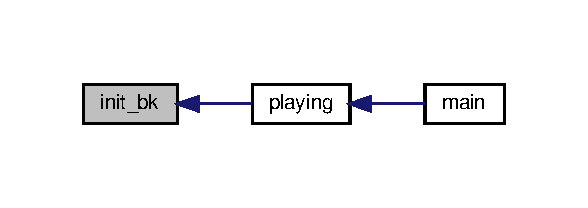
\includegraphics[width=282pt]{background_8h_a64ee95bd1a66087c4ffed437aaa4d550_icgraph}
\end{center}
\end{figure}
\mbox{\Hypertarget{background_8h_a2e14fb88a1bcd685693bb2678f8b50b0}\label{background_8h_a2e14fb88a1bcd685693bb2678f8b50b0}} 
\index{background.\+h@{background.\+h}!scrollingbg@{scrollingbg}}
\index{scrollingbg@{scrollingbg}!background.\+h@{background.\+h}}
\subsubsection{\texorpdfstring{scrollingbg()}{scrollingbg()}}
{\footnotesize\ttfamily void scrollingbg (\begin{DoxyParamCaption}\item[{\hyperlink{structBackground}{Background} $\ast$}]{bg,  }\item[{S\+D\+L\+\_\+\+Surface $\ast$}]{mario,  }\item[{S\+D\+L\+\_\+\+Rect}]{mario\+\_\+position }\end{DoxyParamCaption})}


\hypertarget{bg_8c}{}\section{bg.\+c File Reference}
\label{bg_8c}\index{bg.\+c@{bg.\+c}}
{\ttfamily \#include $<$stdio.\+h$>$}\newline
{\ttfamily \#include $<$S\+D\+L/\+S\+D\+L.\+h$>$}\newline
{\ttfamily \#include $<$stdlib.\+h$>$}\newline
{\ttfamily \#include $<$S\+D\+L/\+S\+D\+L\+\_\+ttf.\+h$>$}\newline
{\ttfamily \#include $<$S\+D\+L/\+S\+D\+L\+\_\+image.\+h$>$}\newline
{\ttfamily \#include \char`\"{}background.\+h\char`\"{}}\newline
{\ttfamily \#include $<$string.\+h$>$}\newline
Include dependency graph for bg.\+c\+:\nopagebreak
\begin{figure}[H]
\begin{center}
\leavevmode
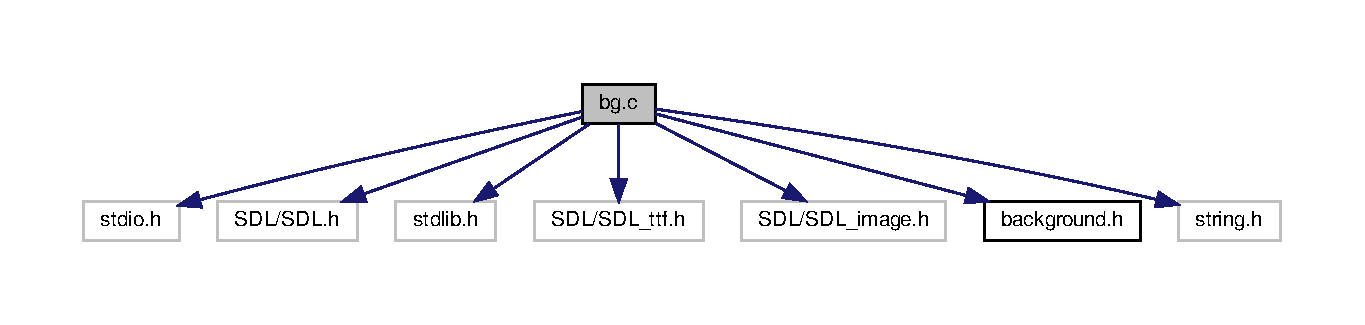
\includegraphics[width=350pt]{bg_8c__incl}
\end{center}
\end{figure}
\subsection*{Functions}
\begin{DoxyCompactItemize}
\item 
void \hyperlink{bg_8c_a64ee95bd1a66087c4ffed437aaa4d550}{init\+\_\+bk} (\hyperlink{structBackground}{Background} $\ast$b)
\end{DoxyCompactItemize}


\subsection{Function Documentation}
\mbox{\Hypertarget{bg_8c_a64ee95bd1a66087c4ffed437aaa4d550}\label{bg_8c_a64ee95bd1a66087c4ffed437aaa4d550}} 
\index{bg.\+c@{bg.\+c}!init\+\_\+bk@{init\+\_\+bk}}
\index{init\+\_\+bk@{init\+\_\+bk}!bg.\+c@{bg.\+c}}
\subsubsection{\texorpdfstring{init\+\_\+bk()}{init\_bk()}}
{\footnotesize\ttfamily void init\+\_\+bk (\begin{DoxyParamCaption}\item[{\hyperlink{structBackground}{Background} $\ast$}]{b }\end{DoxyParamCaption})}

Here is the caller graph for this function\+:\nopagebreak
\begin{figure}[H]
\begin{center}
\leavevmode
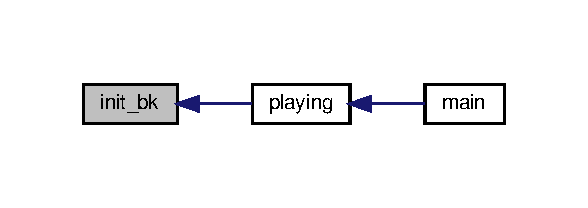
\includegraphics[width=282pt]{bg_8c_a64ee95bd1a66087c4ffed437aaa4d550_icgraph}
\end{center}
\end{figure}

\hypertarget{closhard_8c}{}\section{closhard.\+c File Reference}
\label{closhard_8c}\index{closhard.\+c@{closhard.\+c}}
{\ttfamily \#include $<$S\+D\+L/\+S\+D\+L.\+h$>$}\newline
{\ttfamily \#include $<$S\+D\+L/\+S\+D\+L\+\_\+image.\+h$>$}\newline
{\ttfamily \#include $<$S\+D\+L/\+S\+D\+L\+\_\+ttf.\+h$>$}\newline
{\ttfamily \#include $<$stdlib.\+h$>$}\newline
{\ttfamily \#include $<$stdio.\+h$>$}\newline
{\ttfamily \#include \char`\"{}closhard.\+h\char`\"{}}\newline
Include dependency graph for closhard.\+c\+:\nopagebreak
\begin{figure}[H]
\begin{center}
\leavevmode
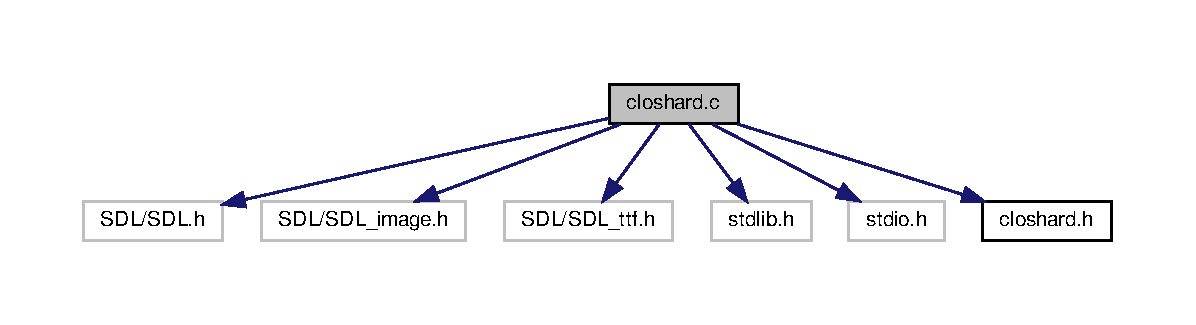
\includegraphics[width=350pt]{closhard_8c__incl}
\end{center}
\end{figure}
\subsection*{Functions}
\begin{DoxyCompactItemize}
\item 
void \hyperlink{closhard_8c_a2a125492867ac06dc538311882f75c43}{C\+L\+O\+C\+H\+A\+R\+D\+\_\+\+Init} (\hyperlink{structClochard}{Clochard} $\ast$c)
\item 
void \hyperlink{closhard_8c_a12a868b46775decd67f2860fe23ed39d}{C\+L\+O\+C\+H\+A\+R\+D\+\_\+\+Render} (\hyperlink{structClochard}{Clochard} $\ast$c, S\+D\+L\+\_\+\+Surface $\ast$$\ast$screen)
\end{DoxyCompactItemize}


\subsection{Function Documentation}
\mbox{\Hypertarget{closhard_8c_a2a125492867ac06dc538311882f75c43}\label{closhard_8c_a2a125492867ac06dc538311882f75c43}} 
\index{closhard.\+c@{closhard.\+c}!C\+L\+O\+C\+H\+A\+R\+D\+\_\+\+Init@{C\+L\+O\+C\+H\+A\+R\+D\+\_\+\+Init}}
\index{C\+L\+O\+C\+H\+A\+R\+D\+\_\+\+Init@{C\+L\+O\+C\+H\+A\+R\+D\+\_\+\+Init}!closhard.\+c@{closhard.\+c}}
\subsubsection{\texorpdfstring{C\+L\+O\+C\+H\+A\+R\+D\+\_\+\+Init()}{CLOCHARD\_Init()}}
{\footnotesize\ttfamily void C\+L\+O\+C\+H\+A\+R\+D\+\_\+\+Init (\begin{DoxyParamCaption}\item[{\hyperlink{structClochard}{Clochard} $\ast$}]{c }\end{DoxyParamCaption})}

Here is the caller graph for this function\+:\nopagebreak
\begin{figure}[H]
\begin{center}
\leavevmode
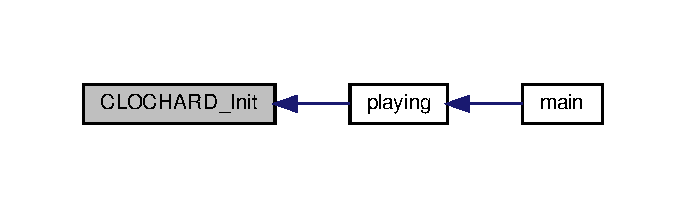
\includegraphics[width=329pt]{closhard_8c_a2a125492867ac06dc538311882f75c43_icgraph}
\end{center}
\end{figure}
\mbox{\Hypertarget{closhard_8c_a12a868b46775decd67f2860fe23ed39d}\label{closhard_8c_a12a868b46775decd67f2860fe23ed39d}} 
\index{closhard.\+c@{closhard.\+c}!C\+L\+O\+C\+H\+A\+R\+D\+\_\+\+Render@{C\+L\+O\+C\+H\+A\+R\+D\+\_\+\+Render}}
\index{C\+L\+O\+C\+H\+A\+R\+D\+\_\+\+Render@{C\+L\+O\+C\+H\+A\+R\+D\+\_\+\+Render}!closhard.\+c@{closhard.\+c}}
\subsubsection{\texorpdfstring{C\+L\+O\+C\+H\+A\+R\+D\+\_\+\+Render()}{CLOCHARD\_Render()}}
{\footnotesize\ttfamily void C\+L\+O\+C\+H\+A\+R\+D\+\_\+\+Render (\begin{DoxyParamCaption}\item[{\hyperlink{structClochard}{Clochard} $\ast$}]{c,  }\item[{S\+D\+L\+\_\+\+Surface $\ast$$\ast$}]{screen }\end{DoxyParamCaption})}

Here is the caller graph for this function\+:\nopagebreak
\begin{figure}[H]
\begin{center}
\leavevmode
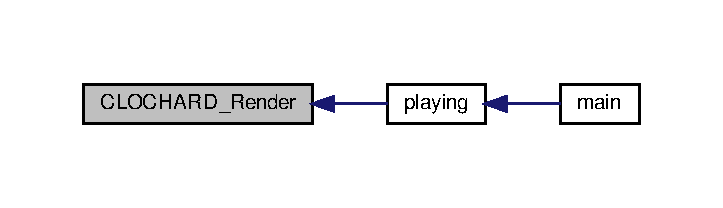
\includegraphics[width=347pt]{closhard_8c_a12a868b46775decd67f2860fe23ed39d_icgraph}
\end{center}
\end{figure}

\hypertarget{closhard_8h}{}\section{closhard.\+h File Reference}
\label{closhard_8h}\index{closhard.\+h@{closhard.\+h}}
This graph shows which files directly or indirectly include this file\+:\nopagebreak
\begin{figure}[H]
\begin{center}
\leavevmode
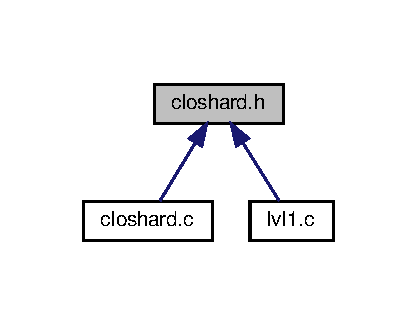
\includegraphics[width=200pt]{closhard_8h__dep__incl}
\end{center}
\end{figure}
\subsection*{Data Structures}
\begin{DoxyCompactItemize}
\item 
struct \hyperlink{structClochard}{Clochard}
\end{DoxyCompactItemize}
\subsection*{Typedefs}
\begin{DoxyCompactItemize}
\item 
typedef struct \hyperlink{structClochard}{Clochard} \hyperlink{closhard_8h_a6dce0477ec4be509d2169f06963520c4}{Clochard}
\end{DoxyCompactItemize}
\subsection*{Functions}
\begin{DoxyCompactItemize}
\item 
void \hyperlink{closhard_8h_a2a125492867ac06dc538311882f75c43}{C\+L\+O\+C\+H\+A\+R\+D\+\_\+\+Init} (\hyperlink{structClochard}{Clochard} $\ast$c)
\item 
void \hyperlink{closhard_8h_a12a868b46775decd67f2860fe23ed39d}{C\+L\+O\+C\+H\+A\+R\+D\+\_\+\+Render} (\hyperlink{structClochard}{Clochard} $\ast$c, S\+D\+L\+\_\+\+Surface $\ast$$\ast$screen)
\end{DoxyCompactItemize}


\subsection{Typedef Documentation}
\mbox{\Hypertarget{closhard_8h_a6dce0477ec4be509d2169f06963520c4}\label{closhard_8h_a6dce0477ec4be509d2169f06963520c4}} 
\index{closhard.\+h@{closhard.\+h}!Clochard@{Clochard}}
\index{Clochard@{Clochard}!closhard.\+h@{closhard.\+h}}
\subsubsection{\texorpdfstring{Clochard}{Clochard}}
{\footnotesize\ttfamily typedef struct \hyperlink{structClochard}{Clochard}  \hyperlink{structClochard}{Clochard}}



\subsection{Function Documentation}
\mbox{\Hypertarget{closhard_8h_a2a125492867ac06dc538311882f75c43}\label{closhard_8h_a2a125492867ac06dc538311882f75c43}} 
\index{closhard.\+h@{closhard.\+h}!C\+L\+O\+C\+H\+A\+R\+D\+\_\+\+Init@{C\+L\+O\+C\+H\+A\+R\+D\+\_\+\+Init}}
\index{C\+L\+O\+C\+H\+A\+R\+D\+\_\+\+Init@{C\+L\+O\+C\+H\+A\+R\+D\+\_\+\+Init}!closhard.\+h@{closhard.\+h}}
\subsubsection{\texorpdfstring{C\+L\+O\+C\+H\+A\+R\+D\+\_\+\+Init()}{CLOCHARD\_Init()}}
{\footnotesize\ttfamily void C\+L\+O\+C\+H\+A\+R\+D\+\_\+\+Init (\begin{DoxyParamCaption}\item[{\hyperlink{structClochard}{Clochard} $\ast$}]{c }\end{DoxyParamCaption})}

Here is the caller graph for this function\+:\nopagebreak
\begin{figure}[H]
\begin{center}
\leavevmode
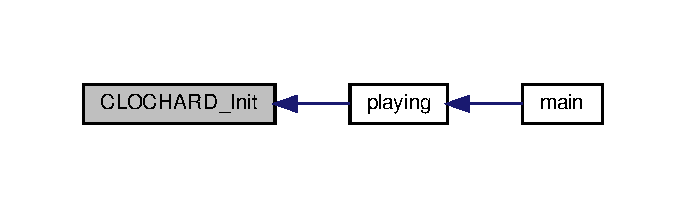
\includegraphics[width=329pt]{closhard_8h_a2a125492867ac06dc538311882f75c43_icgraph}
\end{center}
\end{figure}
\mbox{\Hypertarget{closhard_8h_a12a868b46775decd67f2860fe23ed39d}\label{closhard_8h_a12a868b46775decd67f2860fe23ed39d}} 
\index{closhard.\+h@{closhard.\+h}!C\+L\+O\+C\+H\+A\+R\+D\+\_\+\+Render@{C\+L\+O\+C\+H\+A\+R\+D\+\_\+\+Render}}
\index{C\+L\+O\+C\+H\+A\+R\+D\+\_\+\+Render@{C\+L\+O\+C\+H\+A\+R\+D\+\_\+\+Render}!closhard.\+h@{closhard.\+h}}
\subsubsection{\texorpdfstring{C\+L\+O\+C\+H\+A\+R\+D\+\_\+\+Render()}{CLOCHARD\_Render()}}
{\footnotesize\ttfamily void C\+L\+O\+C\+H\+A\+R\+D\+\_\+\+Render (\begin{DoxyParamCaption}\item[{\hyperlink{structClochard}{Clochard} $\ast$}]{c,  }\item[{S\+D\+L\+\_\+\+Surface $\ast$$\ast$}]{screen }\end{DoxyParamCaption})}

Here is the caller graph for this function\+:\nopagebreak
\begin{figure}[H]
\begin{center}
\leavevmode
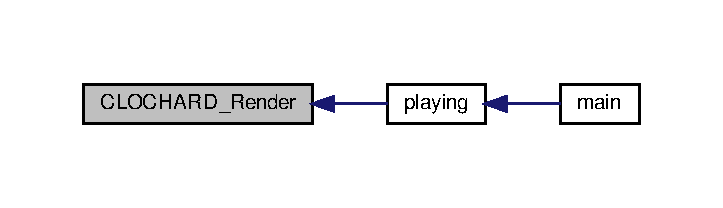
\includegraphics[width=347pt]{closhard_8h_a12a868b46775decd67f2860fe23ed39d_icgraph}
\end{center}
\end{figure}

\hypertarget{colis_8c}{}\section{colis.\+c File Reference}
\label{colis_8c}\index{colis.\+c@{colis.\+c}}
{\ttfamily \#include $<$stdio.\+h$>$}\newline
{\ttfamily \#include $<$S\+D\+L/\+S\+D\+L.\+h$>$}\newline
{\ttfamily \#include $<$stdlib.\+h$>$}\newline
{\ttfamily \#include $<$S\+D\+L/\+S\+D\+L\+\_\+image.\+h$>$}\newline
{\ttfamily \#include \char`\"{}colis.\+h\char`\"{}}\newline
Include dependency graph for colis.\+c\+:\nopagebreak
\begin{figure}[H]
\begin{center}
\leavevmode
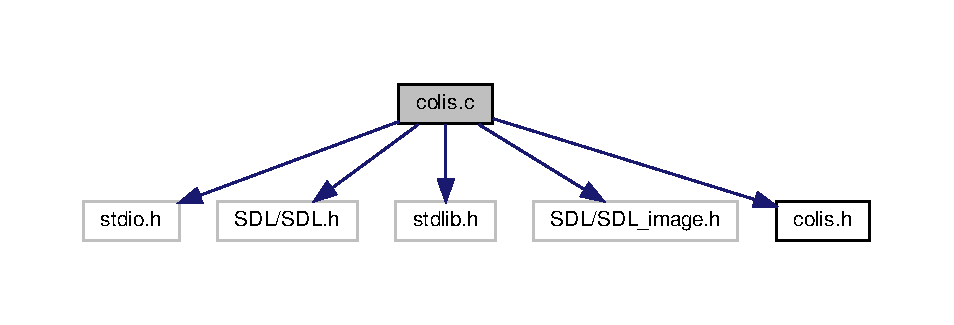
\includegraphics[width=350pt]{colis_8c__incl}
\end{center}
\end{figure}
\subsection*{Functions}
\begin{DoxyCompactItemize}
\item 
S\+D\+L\+\_\+\+Color \hyperlink{colis_8c_a9ec79b71532402381966fc93325d3e52}{Get\+Pixel} (S\+D\+L\+\_\+\+Surface $\ast$p\+Surface, int x, int y)
\item 
int \hyperlink{colis_8c_a632d5ba8a8ddd8a916ba7d835537bf21}{collision\+\_\+parfaite} (S\+D\+L\+\_\+\+Surface $\ast$surfM, S\+D\+L\+\_\+\+Surface $\ast$mario, S\+D\+L\+\_\+\+Rect pos\+\_\+mario, S\+D\+L\+\_\+\+Color co)
\end{DoxyCompactItemize}


\subsection{Function Documentation}
\mbox{\Hypertarget{colis_8c_a632d5ba8a8ddd8a916ba7d835537bf21}\label{colis_8c_a632d5ba8a8ddd8a916ba7d835537bf21}} 
\index{colis.\+c@{colis.\+c}!collision\+\_\+parfaite@{collision\+\_\+parfaite}}
\index{collision\+\_\+parfaite@{collision\+\_\+parfaite}!colis.\+c@{colis.\+c}}
\subsubsection{\texorpdfstring{collision\+\_\+parfaite()}{collision\_parfaite()}}
{\footnotesize\ttfamily int collision\+\_\+parfaite (\begin{DoxyParamCaption}\item[{S\+D\+L\+\_\+\+Surface $\ast$}]{surfM,  }\item[{S\+D\+L\+\_\+\+Surface $\ast$}]{mario,  }\item[{S\+D\+L\+\_\+\+Rect}]{pos\+\_\+mario,  }\item[{S\+D\+L\+\_\+\+Color}]{co }\end{DoxyParamCaption})}

Here is the call graph for this function\+:\nopagebreak
\begin{figure}[H]
\begin{center}
\leavevmode
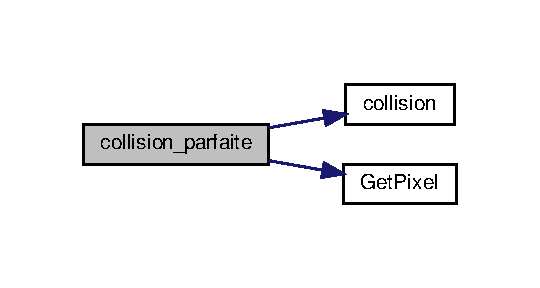
\includegraphics[width=259pt]{colis_8c_a632d5ba8a8ddd8a916ba7d835537bf21_cgraph}
\end{center}
\end{figure}
Here is the caller graph for this function\+:\nopagebreak
\begin{figure}[H]
\begin{center}
\leavevmode
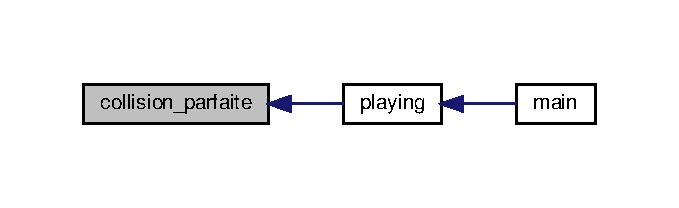
\includegraphics[width=326pt]{colis_8c_a632d5ba8a8ddd8a916ba7d835537bf21_icgraph}
\end{center}
\end{figure}
\mbox{\Hypertarget{colis_8c_a9ec79b71532402381966fc93325d3e52}\label{colis_8c_a9ec79b71532402381966fc93325d3e52}} 
\index{colis.\+c@{colis.\+c}!Get\+Pixel@{Get\+Pixel}}
\index{Get\+Pixel@{Get\+Pixel}!colis.\+c@{colis.\+c}}
\subsubsection{\texorpdfstring{Get\+Pixel()}{GetPixel()}}
{\footnotesize\ttfamily S\+D\+L\+\_\+\+Color Get\+Pixel (\begin{DoxyParamCaption}\item[{S\+D\+L\+\_\+\+Surface $\ast$}]{p\+Surface,  }\item[{int}]{x,  }\item[{int}]{y }\end{DoxyParamCaption})}

Here is the caller graph for this function\+:\nopagebreak
\begin{figure}[H]
\begin{center}
\leavevmode
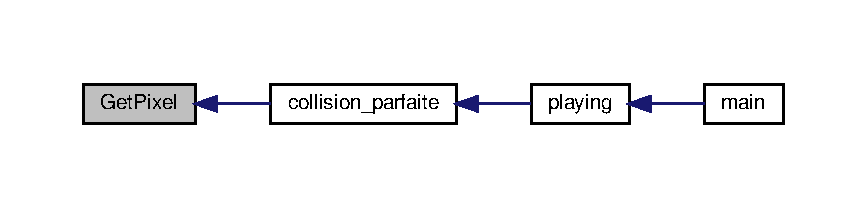
\includegraphics[width=350pt]{colis_8c_a9ec79b71532402381966fc93325d3e52_icgraph}
\end{center}
\end{figure}

\hypertarget{colis_8h}{}\section{colis.\+h File Reference}
\label{colis_8h}\index{colis.\+h@{colis.\+h}}
This graph shows which files directly or indirectly include this file\+:\nopagebreak
\begin{figure}[H]
\begin{center}
\leavevmode
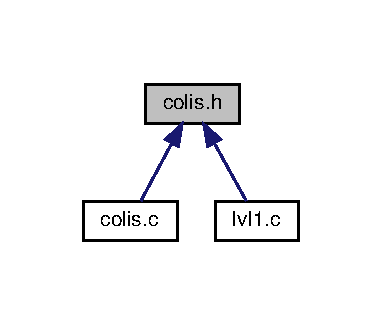
\includegraphics[width=184pt]{colis_8h__dep__incl}
\end{center}
\end{figure}
\subsection*{Functions}
\begin{DoxyCompactItemize}
\item 
int \hyperlink{colis_8h_a632d5ba8a8ddd8a916ba7d835537bf21}{collision\+\_\+parfaite} (S\+D\+L\+\_\+\+Surface $\ast$surfM, S\+D\+L\+\_\+\+Surface $\ast$mario, S\+D\+L\+\_\+\+Rect pos\+\_\+mario, S\+D\+L\+\_\+\+Color co)
\end{DoxyCompactItemize}


\subsection{Function Documentation}
\mbox{\Hypertarget{colis_8h_a632d5ba8a8ddd8a916ba7d835537bf21}\label{colis_8h_a632d5ba8a8ddd8a916ba7d835537bf21}} 
\index{colis.\+h@{colis.\+h}!collision\+\_\+parfaite@{collision\+\_\+parfaite}}
\index{collision\+\_\+parfaite@{collision\+\_\+parfaite}!colis.\+h@{colis.\+h}}
\subsubsection{\texorpdfstring{collision\+\_\+parfaite()}{collision\_parfaite()}}
{\footnotesize\ttfamily int collision\+\_\+parfaite (\begin{DoxyParamCaption}\item[{S\+D\+L\+\_\+\+Surface $\ast$}]{surfM,  }\item[{S\+D\+L\+\_\+\+Surface $\ast$}]{mario,  }\item[{S\+D\+L\+\_\+\+Rect}]{pos\+\_\+mario,  }\item[{S\+D\+L\+\_\+\+Color}]{co }\end{DoxyParamCaption})}

Here is the call graph for this function\+:\nopagebreak
\begin{figure}[H]
\begin{center}
\leavevmode
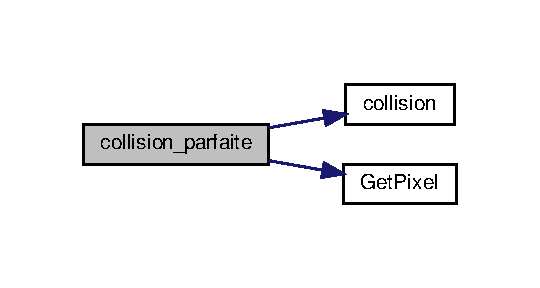
\includegraphics[width=259pt]{colis_8h_a632d5ba8a8ddd8a916ba7d835537bf21_cgraph}
\end{center}
\end{figure}
Here is the caller graph for this function\+:\nopagebreak
\begin{figure}[H]
\begin{center}
\leavevmode
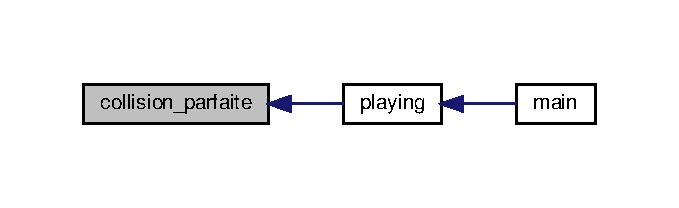
\includegraphics[width=326pt]{colis_8h_a632d5ba8a8ddd8a916ba7d835537bf21_icgraph}
\end{center}
\end{figure}

\hypertarget{collision_8c}{}\section{collision.\+c File Reference}
\label{collision_8c}\index{collision.\+c@{collision.\+c}}
{\ttfamily \#include $<$stdio.\+h$>$}\newline
{\ttfamily \#include $<$S\+D\+L/\+S\+D\+L.\+h$>$}\newline
{\ttfamily \#include $<$stdlib.\+h$>$}\newline
{\ttfamily \#include $<$S\+D\+L/\+S\+D\+L\+\_\+image.\+h$>$}\newline
{\ttfamily \#include \char`\"{}collision.\+h\char`\"{}}\newline
Include dependency graph for collision.\+c\+:\nopagebreak
\begin{figure}[H]
\begin{center}
\leavevmode
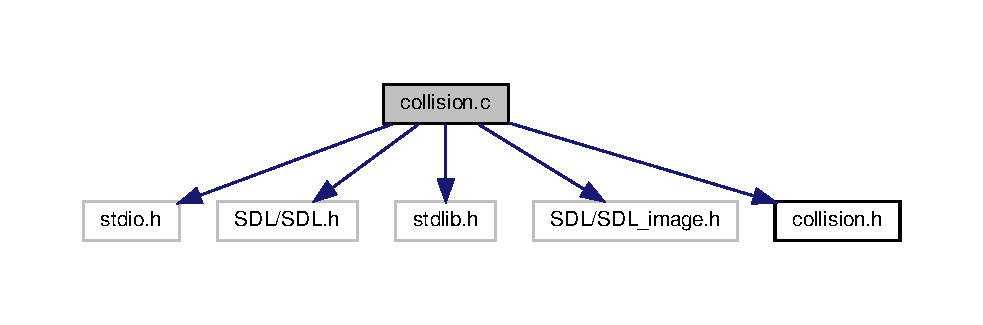
\includegraphics[width=350pt]{collision_8c__incl}
\end{center}
\end{figure}
\subsection*{Functions}
\begin{DoxyCompactItemize}
\item 
int \hyperlink{collision_8c_aa732d1b08f762f8401ec7be13f4b5755}{collision} (S\+D\+L\+\_\+\+Surface $\ast$screen, S\+D\+L\+\_\+\+Rect pos\+\_\+perso, S\+D\+L\+\_\+\+Rect pos\+\_\+obj, int pw, int ph, int ow, int oh)
\end{DoxyCompactItemize}


\subsection{Function Documentation}
\mbox{\Hypertarget{collision_8c_aa732d1b08f762f8401ec7be13f4b5755}\label{collision_8c_aa732d1b08f762f8401ec7be13f4b5755}} 
\index{collision.\+c@{collision.\+c}!collision@{collision}}
\index{collision@{collision}!collision.\+c@{collision.\+c}}
\subsubsection{\texorpdfstring{collision()}{collision()}}
{\footnotesize\ttfamily int collision (\begin{DoxyParamCaption}\item[{S\+D\+L\+\_\+\+Surface $\ast$}]{screen,  }\item[{S\+D\+L\+\_\+\+Rect}]{pos\+\_\+perso,  }\item[{S\+D\+L\+\_\+\+Rect}]{pos\+\_\+obj,  }\item[{int}]{pw,  }\item[{int}]{ph,  }\item[{int}]{ow,  }\item[{int}]{oh }\end{DoxyParamCaption})}

Here is the caller graph for this function\+:\nopagebreak
\begin{figure}[H]
\begin{center}
\leavevmode
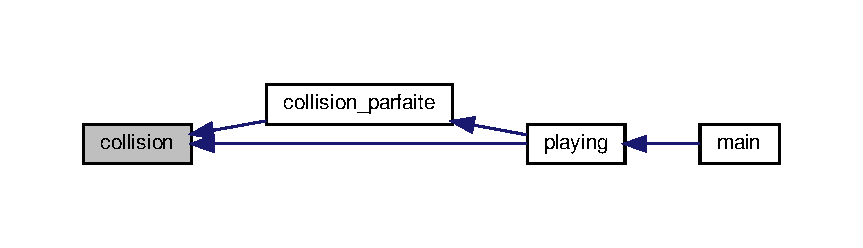
\includegraphics[width=350pt]{collision_8c_aa732d1b08f762f8401ec7be13f4b5755_icgraph}
\end{center}
\end{figure}

\hypertarget{collision_8h}{}\section{collision.\+h File Reference}
\label{collision_8h}\index{collision.\+h@{collision.\+h}}
This graph shows which files directly or indirectly include this file\+:\nopagebreak
\begin{figure}[H]
\begin{center}
\leavevmode
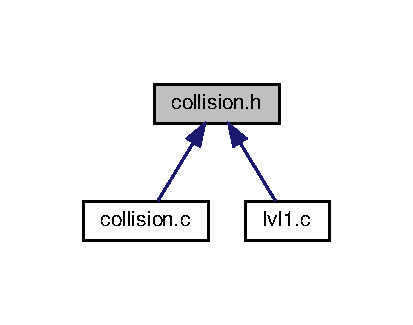
\includegraphics[width=198pt]{collision_8h__dep__incl}
\end{center}
\end{figure}
\subsection*{Functions}
\begin{DoxyCompactItemize}
\item 
int \hyperlink{collision_8h_aa732d1b08f762f8401ec7be13f4b5755}{collision} (S\+D\+L\+\_\+\+Surface $\ast$screen, S\+D\+L\+\_\+\+Rect pos\+\_\+perso, S\+D\+L\+\_\+\+Rect pos\+\_\+obj, int pw, int ph, int ow, int oh)
\end{DoxyCompactItemize}


\subsection{Function Documentation}
\mbox{\Hypertarget{collision_8h_aa732d1b08f762f8401ec7be13f4b5755}\label{collision_8h_aa732d1b08f762f8401ec7be13f4b5755}} 
\index{collision.\+h@{collision.\+h}!collision@{collision}}
\index{collision@{collision}!collision.\+h@{collision.\+h}}
\subsubsection{\texorpdfstring{collision()}{collision()}}
{\footnotesize\ttfamily int collision (\begin{DoxyParamCaption}\item[{S\+D\+L\+\_\+\+Surface $\ast$}]{screen,  }\item[{S\+D\+L\+\_\+\+Rect}]{pos\+\_\+perso,  }\item[{S\+D\+L\+\_\+\+Rect}]{pos\+\_\+obj,  }\item[{int}]{pw,  }\item[{int}]{ph,  }\item[{int}]{ow,  }\item[{int}]{oh }\end{DoxyParamCaption})}

Here is the caller graph for this function\+:\nopagebreak
\begin{figure}[H]
\begin{center}
\leavevmode
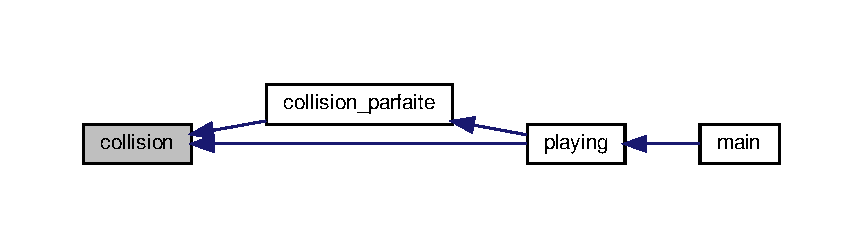
\includegraphics[width=350pt]{collision_8h_aa732d1b08f762f8401ec7be13f4b5755_icgraph}
\end{center}
\end{figure}

\hypertarget{enigme3_8c}{}\section{enigme3.\+c File Reference}
\label{enigme3_8c}\index{enigme3.\+c@{enigme3.\+c}}
{\ttfamily \#include $<$stdlib.\+h$>$}\newline
{\ttfamily \#include $<$stdio.\+h$>$}\newline
{\ttfamily \#include $<$S\+D\+L/\+S\+D\+L\+\_\+mixer.\+h$>$}\newline
{\ttfamily \#include $<$S\+D\+L/\+S\+D\+L\+\_\+image.\+h$>$}\newline
{\ttfamily \#include $<$S\+D\+L/\+S\+D\+L.\+h$>$}\newline
{\ttfamily \#include \char`\"{}enigme3.\+h\char`\"{}}\newline
Include dependency graph for enigme3.\+c\+:\nopagebreak
\begin{figure}[H]
\begin{center}
\leavevmode
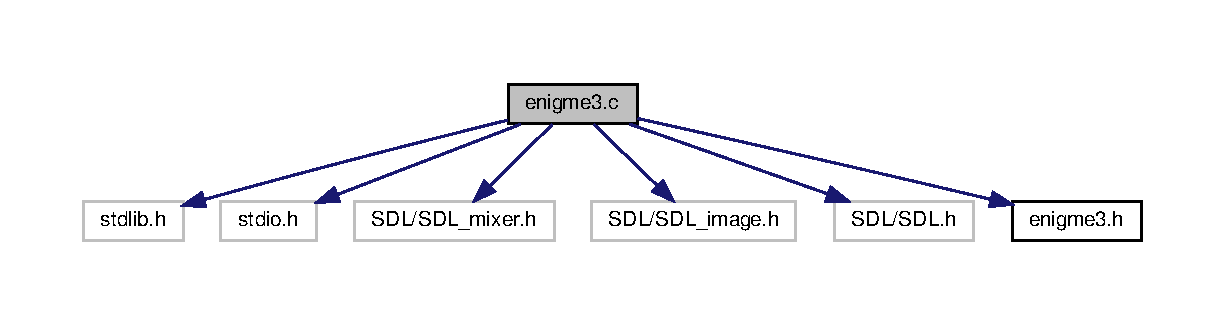
\includegraphics[width=350pt]{enigme3_8c__incl}
\end{center}
\end{figure}
\subsection*{Functions}
\begin{DoxyCompactItemize}
\item 
int \hyperlink{enigme3_8c_a5abbbac61ef3fa3da64f0b297e60e1bc}{resultatenigme3} (char ch\mbox{[}$\,$\mbox{]})
\item 
int \hyperlink{enigme3_8c_ad1de06081817f9aad6c37de5f981e548}{enigme3} (int vie)
\end{DoxyCompactItemize}


\subsection{Function Documentation}
\mbox{\Hypertarget{enigme3_8c_ad1de06081817f9aad6c37de5f981e548}\label{enigme3_8c_ad1de06081817f9aad6c37de5f981e548}} 
\index{enigme3.\+c@{enigme3.\+c}!enigme3@{enigme3}}
\index{enigme3@{enigme3}!enigme3.\+c@{enigme3.\+c}}
\subsubsection{\texorpdfstring{enigme3()}{enigme3()}}
{\footnotesize\ttfamily int enigme3 (\begin{DoxyParamCaption}\item[{int}]{vie }\end{DoxyParamCaption})}

Here is the call graph for this function\+:\nopagebreak
\begin{figure}[H]
\begin{center}
\leavevmode
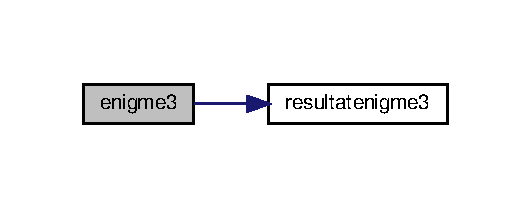
\includegraphics[width=255pt]{enigme3_8c_ad1de06081817f9aad6c37de5f981e548_cgraph}
\end{center}
\end{figure}
Here is the caller graph for this function\+:\nopagebreak
\begin{figure}[H]
\begin{center}
\leavevmode
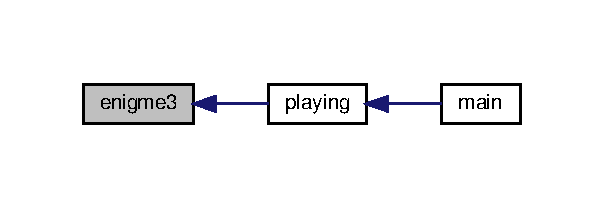
\includegraphics[width=290pt]{enigme3_8c_ad1de06081817f9aad6c37de5f981e548_icgraph}
\end{center}
\end{figure}
\mbox{\Hypertarget{enigme3_8c_a5abbbac61ef3fa3da64f0b297e60e1bc}\label{enigme3_8c_a5abbbac61ef3fa3da64f0b297e60e1bc}} 
\index{enigme3.\+c@{enigme3.\+c}!resultatenigme3@{resultatenigme3}}
\index{resultatenigme3@{resultatenigme3}!enigme3.\+c@{enigme3.\+c}}
\subsubsection{\texorpdfstring{resultatenigme3()}{resultatenigme3()}}
{\footnotesize\ttfamily int resultatenigme3 (\begin{DoxyParamCaption}\item[{char}]{ch\mbox{[}$\,$\mbox{]} }\end{DoxyParamCaption})}

Here is the caller graph for this function\+:\nopagebreak
\begin{figure}[H]
\begin{center}
\leavevmode
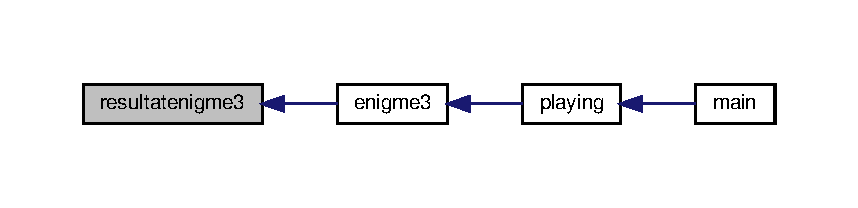
\includegraphics[width=350pt]{enigme3_8c_a5abbbac61ef3fa3da64f0b297e60e1bc_icgraph}
\end{center}
\end{figure}

\hypertarget{enigme3_8h}{}\section{enigme3.\+h File Reference}
\label{enigme3_8h}\index{enigme3.\+h@{enigme3.\+h}}
This graph shows which files directly or indirectly include this file\+:\nopagebreak
\begin{figure}[H]
\begin{center}
\leavevmode
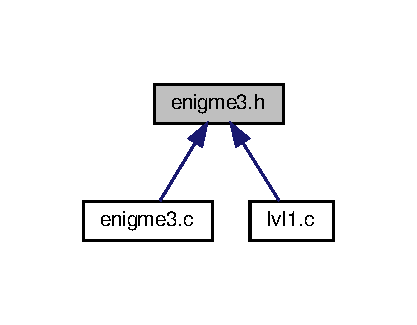
\includegraphics[width=200pt]{enigme3_8h__dep__incl}
\end{center}
\end{figure}
\subsection*{Functions}
\begin{DoxyCompactItemize}
\item 
int \hyperlink{enigme3_8h_ad1de06081817f9aad6c37de5f981e548}{enigme3} (int vie)
\item 
int \hyperlink{enigme3_8h_a5abbbac61ef3fa3da64f0b297e60e1bc}{resultatenigme3} (char ch\mbox{[}$\,$\mbox{]})
\end{DoxyCompactItemize}


\subsection{Function Documentation}
\mbox{\Hypertarget{enigme3_8h_ad1de06081817f9aad6c37de5f981e548}\label{enigme3_8h_ad1de06081817f9aad6c37de5f981e548}} 
\index{enigme3.\+h@{enigme3.\+h}!enigme3@{enigme3}}
\index{enigme3@{enigme3}!enigme3.\+h@{enigme3.\+h}}
\subsubsection{\texorpdfstring{enigme3()}{enigme3()}}
{\footnotesize\ttfamily int enigme3 (\begin{DoxyParamCaption}\item[{int}]{vie }\end{DoxyParamCaption})}

Here is the call graph for this function\+:\nopagebreak
\begin{figure}[H]
\begin{center}
\leavevmode
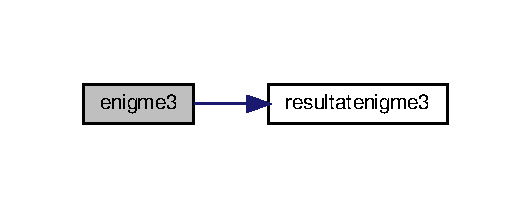
\includegraphics[width=255pt]{enigme3_8h_ad1de06081817f9aad6c37de5f981e548_cgraph}
\end{center}
\end{figure}
Here is the caller graph for this function\+:\nopagebreak
\begin{figure}[H]
\begin{center}
\leavevmode
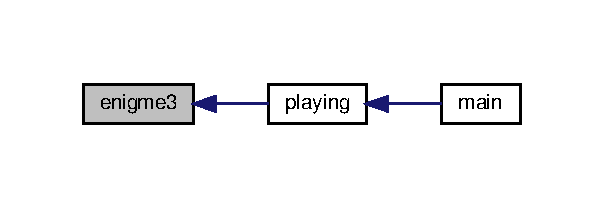
\includegraphics[width=290pt]{enigme3_8h_ad1de06081817f9aad6c37de5f981e548_icgraph}
\end{center}
\end{figure}
\mbox{\Hypertarget{enigme3_8h_a5abbbac61ef3fa3da64f0b297e60e1bc}\label{enigme3_8h_a5abbbac61ef3fa3da64f0b297e60e1bc}} 
\index{enigme3.\+h@{enigme3.\+h}!resultatenigme3@{resultatenigme3}}
\index{resultatenigme3@{resultatenigme3}!enigme3.\+h@{enigme3.\+h}}
\subsubsection{\texorpdfstring{resultatenigme3()}{resultatenigme3()}}
{\footnotesize\ttfamily int resultatenigme3 (\begin{DoxyParamCaption}\item[{char}]{ch\mbox{[}$\,$\mbox{]} }\end{DoxyParamCaption})}

Here is the caller graph for this function\+:\nopagebreak
\begin{figure}[H]
\begin{center}
\leavevmode
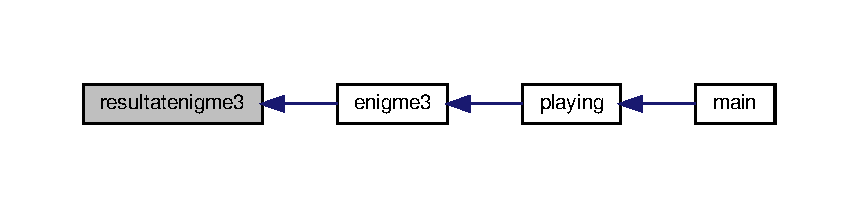
\includegraphics[width=350pt]{enigme3_8h_a5abbbac61ef3fa3da64f0b297e60e1bc_icgraph}
\end{center}
\end{figure}

\hypertarget{hero_8c}{}\section{hero.\+c File Reference}
\label{hero_8c}\index{hero.\+c@{hero.\+c}}
{\ttfamily \#include $<$stdlib.\+h$>$}\newline
{\ttfamily \#include $<$stdio.\+h$>$}\newline
{\ttfamily \#include $<$S\+D\+L/\+S\+D\+L.\+h$>$}\newline
{\ttfamily \#include $<$S\+D\+L/\+S\+D\+L\+\_\+image.\+h$>$}\newline
{\ttfamily \#include \char`\"{}hero.\+h\char`\"{}}\newline
Include dependency graph for hero.\+c\+:\nopagebreak
\begin{figure}[H]
\begin{center}
\leavevmode
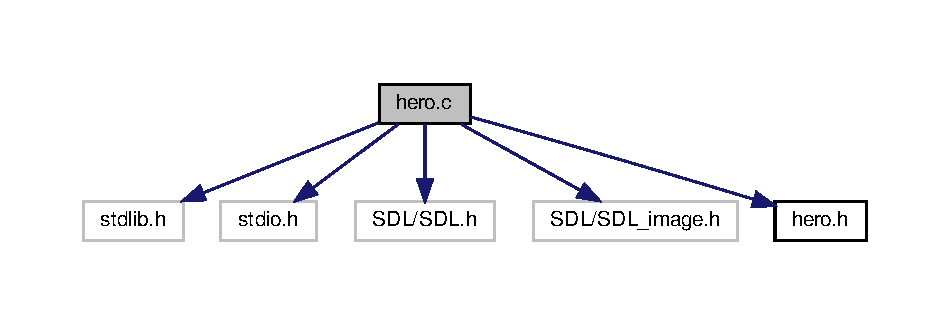
\includegraphics[width=350pt]{hero_8c__incl}
\end{center}
\end{figure}
\subsection*{Functions}
\begin{DoxyCompactItemize}
\item 
void \hyperlink{hero_8c_a38a0e5acc6bc70e6ba633614600ec9d7}{init} (\hyperlink{structhero}{hero} $\ast$\hyperlink{structhero}{hero})
\item 
void \hyperlink{hero_8c_a624f766b1ff0fa9fff0468f08844ce3a}{init2} (\hyperlink{structhero}{hero} $\ast$\hyperlink{structhero}{hero})
\item 
void \hyperlink{hero_8c_a057811a3d9cd58ff9b99c43d42149a7f}{setright} (\hyperlink{structhero}{hero} $\ast$\hyperlink{structhero}{hero})
\item 
void \hyperlink{hero_8c_af7a30def34c0c79cae07e178561252e1}{setleft} (\hyperlink{structhero}{hero} $\ast$\hyperlink{structhero}{hero})
\item 
void \hyperlink{hero_8c_a64b930ab443d9a341610887cb03af8da}{deplacerhero} (\hyperlink{structhero}{hero} $\ast$\hyperlink{structhero}{hero})
\item 
void \hyperlink{hero_8c_aa0c6e17abebb653e823a7f48b153b44b}{blithero} (\hyperlink{structhero}{hero} $\ast$\hyperlink{structhero}{hero}, S\+D\+L\+\_\+\+Surface $\ast$screen, int choix)
\item 
void \hyperlink{hero_8c_a47d78c641261389245a34c8484662075}{jump} (\hyperlink{structhero}{hero} $\ast$\hyperlink{structhero}{hero})
\item 
void \hyperlink{hero_8c_ab28b973e75d358056e611bc586fd89e3}{donejumping} (\hyperlink{structhero}{hero} $\ast$\hyperlink{structhero}{hero})
\item 
void \hyperlink{hero_8c_af75055a4383728ef90eea68b82747196}{initminimap} (\hyperlink{hero_8h_a0e4a13c54ca0b78464c35eafd50d7d60}{mm} $\ast$m)
\item 
void \hyperlink{hero_8c_a4ada4b1d3752fff626bfa1d506cb63df}{blitminimap} (\hyperlink{hero_8h_a0e4a13c54ca0b78464c35eafd50d7d60}{mm} $\ast$m, S\+D\+L\+\_\+\+Surface $\ast$screen, int choix)
\item 
void \hyperlink{hero_8c_afbecac4a8134947583d06051cb683c69}{deplacementminihero} (\hyperlink{hero_8h_a0e4a13c54ca0b78464c35eafd50d7d60}{mm} $\ast$m, int direction)
\end{DoxyCompactItemize}


\subsection{Function Documentation}
\mbox{\Hypertarget{hero_8c_aa0c6e17abebb653e823a7f48b153b44b}\label{hero_8c_aa0c6e17abebb653e823a7f48b153b44b}} 
\index{hero.\+c@{hero.\+c}!blithero@{blithero}}
\index{blithero@{blithero}!hero.\+c@{hero.\+c}}
\subsubsection{\texorpdfstring{blithero()}{blithero()}}
{\footnotesize\ttfamily void blithero (\begin{DoxyParamCaption}\item[{\hyperlink{structhero}{hero} $\ast$}]{hero,  }\item[{S\+D\+L\+\_\+\+Surface $\ast$}]{screen,  }\item[{int}]{choix }\end{DoxyParamCaption})}

Here is the caller graph for this function\+:\nopagebreak
\begin{figure}[H]
\begin{center}
\leavevmode
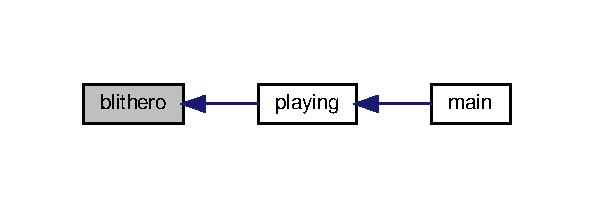
\includegraphics[width=285pt]{hero_8c_aa0c6e17abebb653e823a7f48b153b44b_icgraph}
\end{center}
\end{figure}
\mbox{\Hypertarget{hero_8c_a4ada4b1d3752fff626bfa1d506cb63df}\label{hero_8c_a4ada4b1d3752fff626bfa1d506cb63df}} 
\index{hero.\+c@{hero.\+c}!blitminimap@{blitminimap}}
\index{blitminimap@{blitminimap}!hero.\+c@{hero.\+c}}
\subsubsection{\texorpdfstring{blitminimap()}{blitminimap()}}
{\footnotesize\ttfamily void blitminimap (\begin{DoxyParamCaption}\item[{\hyperlink{hero_8h_a0e4a13c54ca0b78464c35eafd50d7d60}{mm} $\ast$}]{m,  }\item[{S\+D\+L\+\_\+\+Surface $\ast$}]{screen,  }\item[{int}]{choix }\end{DoxyParamCaption})}

Here is the call graph for this function\+:\nopagebreak
\begin{figure}[H]
\begin{center}
\leavevmode
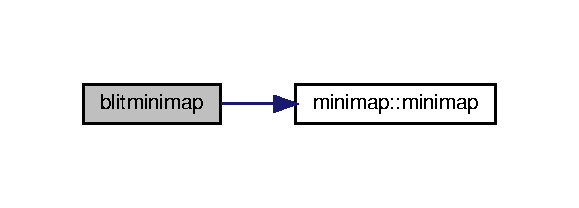
\includegraphics[width=278pt]{hero_8c_a4ada4b1d3752fff626bfa1d506cb63df_cgraph}
\end{center}
\end{figure}
Here is the caller graph for this function\+:\nopagebreak
\begin{figure}[H]
\begin{center}
\leavevmode
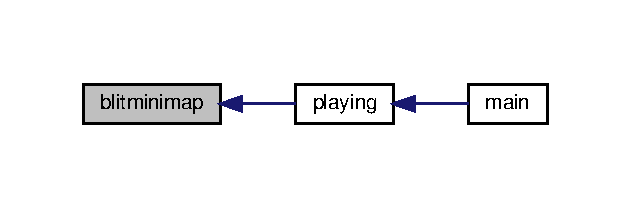
\includegraphics[width=303pt]{hero_8c_a4ada4b1d3752fff626bfa1d506cb63df_icgraph}
\end{center}
\end{figure}
\mbox{\Hypertarget{hero_8c_afbecac4a8134947583d06051cb683c69}\label{hero_8c_afbecac4a8134947583d06051cb683c69}} 
\index{hero.\+c@{hero.\+c}!deplacementminihero@{deplacementminihero}}
\index{deplacementminihero@{deplacementminihero}!hero.\+c@{hero.\+c}}
\subsubsection{\texorpdfstring{deplacementminihero()}{deplacementminihero()}}
{\footnotesize\ttfamily void deplacementminihero (\begin{DoxyParamCaption}\item[{\hyperlink{hero_8h_a0e4a13c54ca0b78464c35eafd50d7d60}{mm} $\ast$}]{m,  }\item[{int}]{direction }\end{DoxyParamCaption})}

Here is the caller graph for this function\+:\nopagebreak
\begin{figure}[H]
\begin{center}
\leavevmode
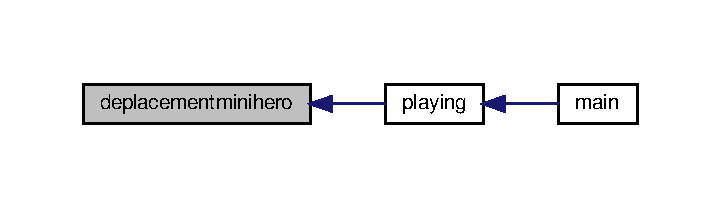
\includegraphics[width=346pt]{hero_8c_afbecac4a8134947583d06051cb683c69_icgraph}
\end{center}
\end{figure}
\mbox{\Hypertarget{hero_8c_a64b930ab443d9a341610887cb03af8da}\label{hero_8c_a64b930ab443d9a341610887cb03af8da}} 
\index{hero.\+c@{hero.\+c}!deplacerhero@{deplacerhero}}
\index{deplacerhero@{deplacerhero}!hero.\+c@{hero.\+c}}
\subsubsection{\texorpdfstring{deplacerhero()}{deplacerhero()}}
{\footnotesize\ttfamily void deplacerhero (\begin{DoxyParamCaption}\item[{\hyperlink{structhero}{hero} $\ast$}]{hero }\end{DoxyParamCaption})}

Here is the caller graph for this function\+:\nopagebreak
\begin{figure}[H]
\begin{center}
\leavevmode
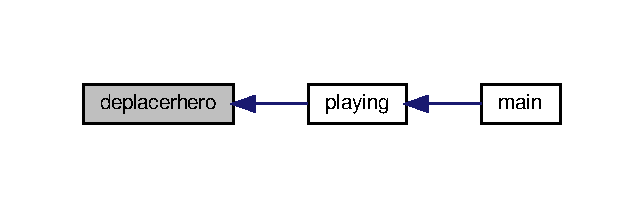
\includegraphics[width=309pt]{hero_8c_a64b930ab443d9a341610887cb03af8da_icgraph}
\end{center}
\end{figure}
\mbox{\Hypertarget{hero_8c_ab28b973e75d358056e611bc586fd89e3}\label{hero_8c_ab28b973e75d358056e611bc586fd89e3}} 
\index{hero.\+c@{hero.\+c}!donejumping@{donejumping}}
\index{donejumping@{donejumping}!hero.\+c@{hero.\+c}}
\subsubsection{\texorpdfstring{donejumping()}{donejumping()}}
{\footnotesize\ttfamily void donejumping (\begin{DoxyParamCaption}\item[{\hyperlink{structhero}{hero} $\ast$}]{hero }\end{DoxyParamCaption})}

Here is the caller graph for this function\+:\nopagebreak
\begin{figure}[H]
\begin{center}
\leavevmode
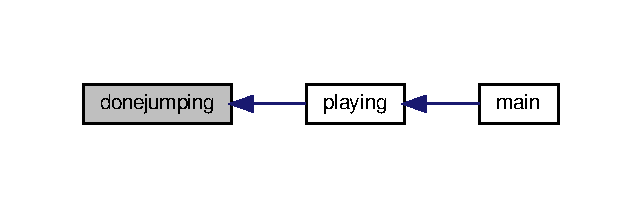
\includegraphics[width=308pt]{hero_8c_ab28b973e75d358056e611bc586fd89e3_icgraph}
\end{center}
\end{figure}
\mbox{\Hypertarget{hero_8c_a38a0e5acc6bc70e6ba633614600ec9d7}\label{hero_8c_a38a0e5acc6bc70e6ba633614600ec9d7}} 
\index{hero.\+c@{hero.\+c}!init@{init}}
\index{init@{init}!hero.\+c@{hero.\+c}}
\subsubsection{\texorpdfstring{init()}{init()}}
{\footnotesize\ttfamily void init (\begin{DoxyParamCaption}\item[{\hyperlink{structhero}{hero} $\ast$}]{hero }\end{DoxyParamCaption})}

Here is the caller graph for this function\+:\nopagebreak
\begin{figure}[H]
\begin{center}
\leavevmode
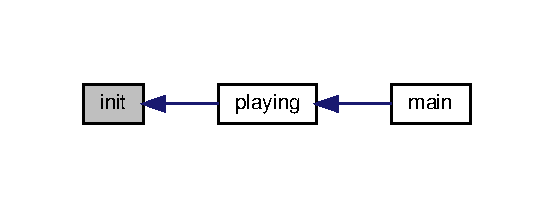
\includegraphics[width=266pt]{hero_8c_a38a0e5acc6bc70e6ba633614600ec9d7_icgraph}
\end{center}
\end{figure}
\mbox{\Hypertarget{hero_8c_a624f766b1ff0fa9fff0468f08844ce3a}\label{hero_8c_a624f766b1ff0fa9fff0468f08844ce3a}} 
\index{hero.\+c@{hero.\+c}!init2@{init2}}
\index{init2@{init2}!hero.\+c@{hero.\+c}}
\subsubsection{\texorpdfstring{init2()}{init2()}}
{\footnotesize\ttfamily void init2 (\begin{DoxyParamCaption}\item[{\hyperlink{structhero}{hero} $\ast$}]{hero }\end{DoxyParamCaption})}

Here is the caller graph for this function\+:\nopagebreak
\begin{figure}[H]
\begin{center}
\leavevmode
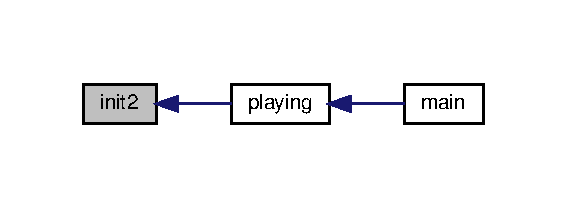
\includegraphics[width=272pt]{hero_8c_a624f766b1ff0fa9fff0468f08844ce3a_icgraph}
\end{center}
\end{figure}
\mbox{\Hypertarget{hero_8c_af75055a4383728ef90eea68b82747196}\label{hero_8c_af75055a4383728ef90eea68b82747196}} 
\index{hero.\+c@{hero.\+c}!initminimap@{initminimap}}
\index{initminimap@{initminimap}!hero.\+c@{hero.\+c}}
\subsubsection{\texorpdfstring{initminimap()}{initminimap()}}
{\footnotesize\ttfamily void initminimap (\begin{DoxyParamCaption}\item[{\hyperlink{hero_8h_a0e4a13c54ca0b78464c35eafd50d7d60}{mm} $\ast$}]{m }\end{DoxyParamCaption})}

Here is the call graph for this function\+:\nopagebreak
\begin{figure}[H]
\begin{center}
\leavevmode
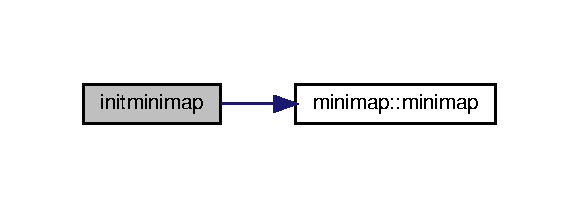
\includegraphics[width=278pt]{hero_8c_af75055a4383728ef90eea68b82747196_cgraph}
\end{center}
\end{figure}
Here is the caller graph for this function\+:\nopagebreak
\begin{figure}[H]
\begin{center}
\leavevmode
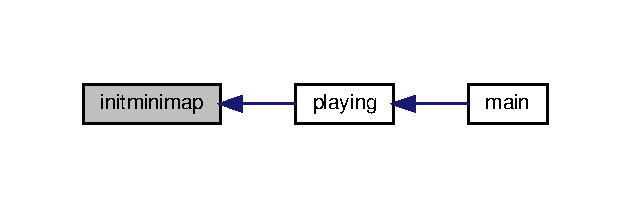
\includegraphics[width=303pt]{hero_8c_af75055a4383728ef90eea68b82747196_icgraph}
\end{center}
\end{figure}
\mbox{\Hypertarget{hero_8c_a47d78c641261389245a34c8484662075}\label{hero_8c_a47d78c641261389245a34c8484662075}} 
\index{hero.\+c@{hero.\+c}!jump@{jump}}
\index{jump@{jump}!hero.\+c@{hero.\+c}}
\subsubsection{\texorpdfstring{jump()}{jump()}}
{\footnotesize\ttfamily void jump (\begin{DoxyParamCaption}\item[{\hyperlink{structhero}{hero} $\ast$}]{hero }\end{DoxyParamCaption})}

Here is the caller graph for this function\+:\nopagebreak
\begin{figure}[H]
\begin{center}
\leavevmode
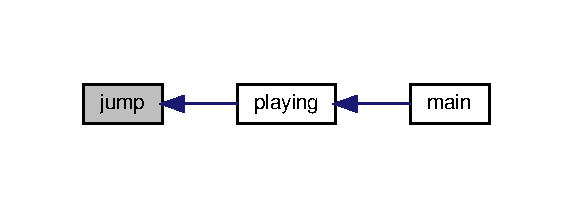
\includegraphics[width=275pt]{hero_8c_a47d78c641261389245a34c8484662075_icgraph}
\end{center}
\end{figure}
\mbox{\Hypertarget{hero_8c_af7a30def34c0c79cae07e178561252e1}\label{hero_8c_af7a30def34c0c79cae07e178561252e1}} 
\index{hero.\+c@{hero.\+c}!setleft@{setleft}}
\index{setleft@{setleft}!hero.\+c@{hero.\+c}}
\subsubsection{\texorpdfstring{setleft()}{setleft()}}
{\footnotesize\ttfamily void setleft (\begin{DoxyParamCaption}\item[{\hyperlink{structhero}{hero} $\ast$}]{hero }\end{DoxyParamCaption})}

Here is the caller graph for this function\+:\nopagebreak
\begin{figure}[H]
\begin{center}
\leavevmode
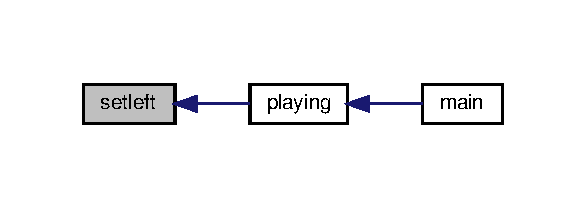
\includegraphics[width=281pt]{hero_8c_af7a30def34c0c79cae07e178561252e1_icgraph}
\end{center}
\end{figure}
\mbox{\Hypertarget{hero_8c_a057811a3d9cd58ff9b99c43d42149a7f}\label{hero_8c_a057811a3d9cd58ff9b99c43d42149a7f}} 
\index{hero.\+c@{hero.\+c}!setright@{setright}}
\index{setright@{setright}!hero.\+c@{hero.\+c}}
\subsubsection{\texorpdfstring{setright()}{setright()}}
{\footnotesize\ttfamily void setright (\begin{DoxyParamCaption}\item[{\hyperlink{structhero}{hero} $\ast$}]{hero }\end{DoxyParamCaption})}

Here is the caller graph for this function\+:\nopagebreak
\begin{figure}[H]
\begin{center}
\leavevmode
\includegraphics[width=286pt]{hero_8c_a057811a3d9cd58ff9b99c43d42149a7f_icgraph}
\end{center}
\end{figure}

\hypertarget{hero_8h}{}\section{hero.\+h File Reference}
\label{hero_8h}\index{hero.\+h@{hero.\+h}}
This graph shows which files directly or indirectly include this file\+:\nopagebreak
\begin{figure}[H]
\begin{center}
\leavevmode
\includegraphics[width=268pt]{hero_8h__dep__incl}
\end{center}
\end{figure}
\subsection*{Data Structures}
\begin{DoxyCompactItemize}
\item 
struct \hyperlink{structhero}{hero}
\item 
struct \hyperlink{structminimap}{minimap}
\end{DoxyCompactItemize}
\subsection*{Typedefs}
\begin{DoxyCompactItemize}
\item 
typedef struct \hyperlink{structhero}{hero} \hyperlink{hero_8h_ab00d3f853a1dee57c09253477c55276e}{hero}
\item 
typedef struct \hyperlink{structminimap}{minimap} \hyperlink{hero_8h_a0e4a13c54ca0b78464c35eafd50d7d60}{mm}
\end{DoxyCompactItemize}
\subsection*{Functions}
\begin{DoxyCompactItemize}
\item 
void \hyperlink{hero_8h_a38a0e5acc6bc70e6ba633614600ec9d7}{init} (\hyperlink{structhero}{hero} $\ast$\hyperlink{structhero}{hero})
\item 
void \hyperlink{hero_8h_a624f766b1ff0fa9fff0468f08844ce3a}{init2} (\hyperlink{structhero}{hero} $\ast$\hyperlink{structhero}{hero})
\item 
void \hyperlink{hero_8h_a057811a3d9cd58ff9b99c43d42149a7f}{setright} (\hyperlink{structhero}{hero} $\ast$\hyperlink{structhero}{hero})
\item 
void \hyperlink{hero_8h_af7a30def34c0c79cae07e178561252e1}{setleft} (\hyperlink{structhero}{hero} $\ast$\hyperlink{structhero}{hero})
\item 
void \hyperlink{hero_8h_a64b930ab443d9a341610887cb03af8da}{deplacerhero} (\hyperlink{structhero}{hero} $\ast$\hyperlink{structhero}{hero})
\item 
void \hyperlink{hero_8h_aa0c6e17abebb653e823a7f48b153b44b}{blithero} (\hyperlink{structhero}{hero} $\ast$\hyperlink{structhero}{hero}, S\+D\+L\+\_\+\+Surface $\ast$screen, int choix)
\item 
void \hyperlink{hero_8h_a47d78c641261389245a34c8484662075}{jump} (\hyperlink{structhero}{hero} $\ast$\hyperlink{structhero}{hero})
\item 
void \hyperlink{hero_8h_ab28b973e75d358056e611bc586fd89e3}{donejumping} (\hyperlink{structhero}{hero} $\ast$\hyperlink{structhero}{hero})
\item 
void \hyperlink{hero_8h_af75055a4383728ef90eea68b82747196}{initminimap} (\hyperlink{hero_8h_a0e4a13c54ca0b78464c35eafd50d7d60}{mm} $\ast$m)
\item 
void \hyperlink{hero_8h_a4ada4b1d3752fff626bfa1d506cb63df}{blitminimap} (\hyperlink{hero_8h_a0e4a13c54ca0b78464c35eafd50d7d60}{mm} $\ast$m, S\+D\+L\+\_\+\+Surface $\ast$screen, int choix)
\item 
void \hyperlink{hero_8h_afbecac4a8134947583d06051cb683c69}{deplacementminihero} (\hyperlink{hero_8h_a0e4a13c54ca0b78464c35eafd50d7d60}{mm} $\ast$m, int direction)
\item 
int \hyperlink{hero_8h_ab5e525dc5214e074daa84bcab6f95839}{playing} (S\+D\+L\+\_\+\+Surface $\ast$screen, int ou, int perso, int cc, int mini, int pos\+\_\+cam, int score, int nb\+\_\+vie, int time, int pos\+\_\+perso, int test)
\end{DoxyCompactItemize}


\subsection{Typedef Documentation}
\mbox{\Hypertarget{hero_8h_ab00d3f853a1dee57c09253477c55276e}\label{hero_8h_ab00d3f853a1dee57c09253477c55276e}} 
\index{hero.\+h@{hero.\+h}!hero@{hero}}
\index{hero@{hero}!hero.\+h@{hero.\+h}}
\subsubsection{\texorpdfstring{hero}{hero}}
{\footnotesize\ttfamily typedef struct \hyperlink{structhero}{hero} \hyperlink{structhero}{hero}}

\mbox{\Hypertarget{hero_8h_a0e4a13c54ca0b78464c35eafd50d7d60}\label{hero_8h_a0e4a13c54ca0b78464c35eafd50d7d60}} 
\index{hero.\+h@{hero.\+h}!mm@{mm}}
\index{mm@{mm}!hero.\+h@{hero.\+h}}
\subsubsection{\texorpdfstring{mm}{mm}}
{\footnotesize\ttfamily typedef struct \hyperlink{structminimap}{minimap} \hyperlink{hero_8h_a0e4a13c54ca0b78464c35eafd50d7d60}{mm}}



\subsection{Function Documentation}
\mbox{\Hypertarget{hero_8h_aa0c6e17abebb653e823a7f48b153b44b}\label{hero_8h_aa0c6e17abebb653e823a7f48b153b44b}} 
\index{hero.\+h@{hero.\+h}!blithero@{blithero}}
\index{blithero@{blithero}!hero.\+h@{hero.\+h}}
\subsubsection{\texorpdfstring{blithero()}{blithero()}}
{\footnotesize\ttfamily void blithero (\begin{DoxyParamCaption}\item[{\hyperlink{structhero}{hero} $\ast$}]{hero,  }\item[{S\+D\+L\+\_\+\+Surface $\ast$}]{screen,  }\item[{int}]{choix }\end{DoxyParamCaption})}

Here is the caller graph for this function\+:\nopagebreak
\begin{figure}[H]
\begin{center}
\leavevmode
\includegraphics[width=285pt]{hero_8h_aa0c6e17abebb653e823a7f48b153b44b_icgraph}
\end{center}
\end{figure}
\mbox{\Hypertarget{hero_8h_a4ada4b1d3752fff626bfa1d506cb63df}\label{hero_8h_a4ada4b1d3752fff626bfa1d506cb63df}} 
\index{hero.\+h@{hero.\+h}!blitminimap@{blitminimap}}
\index{blitminimap@{blitminimap}!hero.\+h@{hero.\+h}}
\subsubsection{\texorpdfstring{blitminimap()}{blitminimap()}}
{\footnotesize\ttfamily void blitminimap (\begin{DoxyParamCaption}\item[{\hyperlink{hero_8h_a0e4a13c54ca0b78464c35eafd50d7d60}{mm} $\ast$}]{m,  }\item[{S\+D\+L\+\_\+\+Surface $\ast$}]{screen,  }\item[{int}]{choix }\end{DoxyParamCaption})}

Here is the call graph for this function\+:\nopagebreak
\begin{figure}[H]
\begin{center}
\leavevmode
\includegraphics[width=278pt]{hero_8h_a4ada4b1d3752fff626bfa1d506cb63df_cgraph}
\end{center}
\end{figure}
Here is the caller graph for this function\+:\nopagebreak
\begin{figure}[H]
\begin{center}
\leavevmode
\includegraphics[width=303pt]{hero_8h_a4ada4b1d3752fff626bfa1d506cb63df_icgraph}
\end{center}
\end{figure}
\mbox{\Hypertarget{hero_8h_afbecac4a8134947583d06051cb683c69}\label{hero_8h_afbecac4a8134947583d06051cb683c69}} 
\index{hero.\+h@{hero.\+h}!deplacementminihero@{deplacementminihero}}
\index{deplacementminihero@{deplacementminihero}!hero.\+h@{hero.\+h}}
\subsubsection{\texorpdfstring{deplacementminihero()}{deplacementminihero()}}
{\footnotesize\ttfamily void deplacementminihero (\begin{DoxyParamCaption}\item[{\hyperlink{hero_8h_a0e4a13c54ca0b78464c35eafd50d7d60}{mm} $\ast$}]{m,  }\item[{int}]{direction }\end{DoxyParamCaption})}

Here is the caller graph for this function\+:\nopagebreak
\begin{figure}[H]
\begin{center}
\leavevmode
\includegraphics[width=346pt]{hero_8h_afbecac4a8134947583d06051cb683c69_icgraph}
\end{center}
\end{figure}
\mbox{\Hypertarget{hero_8h_a64b930ab443d9a341610887cb03af8da}\label{hero_8h_a64b930ab443d9a341610887cb03af8da}} 
\index{hero.\+h@{hero.\+h}!deplacerhero@{deplacerhero}}
\index{deplacerhero@{deplacerhero}!hero.\+h@{hero.\+h}}
\subsubsection{\texorpdfstring{deplacerhero()}{deplacerhero()}}
{\footnotesize\ttfamily void deplacerhero (\begin{DoxyParamCaption}\item[{\hyperlink{structhero}{hero} $\ast$}]{hero }\end{DoxyParamCaption})}

Here is the caller graph for this function\+:\nopagebreak
\begin{figure}[H]
\begin{center}
\leavevmode
\includegraphics[width=309pt]{hero_8h_a64b930ab443d9a341610887cb03af8da_icgraph}
\end{center}
\end{figure}
\mbox{\Hypertarget{hero_8h_ab28b973e75d358056e611bc586fd89e3}\label{hero_8h_ab28b973e75d358056e611bc586fd89e3}} 
\index{hero.\+h@{hero.\+h}!donejumping@{donejumping}}
\index{donejumping@{donejumping}!hero.\+h@{hero.\+h}}
\subsubsection{\texorpdfstring{donejumping()}{donejumping()}}
{\footnotesize\ttfamily void donejumping (\begin{DoxyParamCaption}\item[{\hyperlink{structhero}{hero} $\ast$}]{hero }\end{DoxyParamCaption})}

Here is the caller graph for this function\+:\nopagebreak
\begin{figure}[H]
\begin{center}
\leavevmode
\includegraphics[width=308pt]{hero_8h_ab28b973e75d358056e611bc586fd89e3_icgraph}
\end{center}
\end{figure}
\mbox{\Hypertarget{hero_8h_a38a0e5acc6bc70e6ba633614600ec9d7}\label{hero_8h_a38a0e5acc6bc70e6ba633614600ec9d7}} 
\index{hero.\+h@{hero.\+h}!init@{init}}
\index{init@{init}!hero.\+h@{hero.\+h}}
\subsubsection{\texorpdfstring{init()}{init()}}
{\footnotesize\ttfamily void init (\begin{DoxyParamCaption}\item[{\hyperlink{structhero}{hero} $\ast$}]{hero }\end{DoxyParamCaption})}

Here is the caller graph for this function\+:\nopagebreak
\begin{figure}[H]
\begin{center}
\leavevmode
\includegraphics[width=266pt]{hero_8h_a38a0e5acc6bc70e6ba633614600ec9d7_icgraph}
\end{center}
\end{figure}
\mbox{\Hypertarget{hero_8h_a624f766b1ff0fa9fff0468f08844ce3a}\label{hero_8h_a624f766b1ff0fa9fff0468f08844ce3a}} 
\index{hero.\+h@{hero.\+h}!init2@{init2}}
\index{init2@{init2}!hero.\+h@{hero.\+h}}
\subsubsection{\texorpdfstring{init2()}{init2()}}
{\footnotesize\ttfamily void init2 (\begin{DoxyParamCaption}\item[{\hyperlink{structhero}{hero} $\ast$}]{hero }\end{DoxyParamCaption})}

Here is the caller graph for this function\+:\nopagebreak
\begin{figure}[H]
\begin{center}
\leavevmode
\includegraphics[width=272pt]{hero_8h_a624f766b1ff0fa9fff0468f08844ce3a_icgraph}
\end{center}
\end{figure}
\mbox{\Hypertarget{hero_8h_af75055a4383728ef90eea68b82747196}\label{hero_8h_af75055a4383728ef90eea68b82747196}} 
\index{hero.\+h@{hero.\+h}!initminimap@{initminimap}}
\index{initminimap@{initminimap}!hero.\+h@{hero.\+h}}
\subsubsection{\texorpdfstring{initminimap()}{initminimap()}}
{\footnotesize\ttfamily void initminimap (\begin{DoxyParamCaption}\item[{\hyperlink{hero_8h_a0e4a13c54ca0b78464c35eafd50d7d60}{mm} $\ast$}]{m }\end{DoxyParamCaption})}

Here is the call graph for this function\+:\nopagebreak
\begin{figure}[H]
\begin{center}
\leavevmode
\includegraphics[width=278pt]{hero_8h_af75055a4383728ef90eea68b82747196_cgraph}
\end{center}
\end{figure}
Here is the caller graph for this function\+:\nopagebreak
\begin{figure}[H]
\begin{center}
\leavevmode
\includegraphics[width=303pt]{hero_8h_af75055a4383728ef90eea68b82747196_icgraph}
\end{center}
\end{figure}
\mbox{\Hypertarget{hero_8h_a47d78c641261389245a34c8484662075}\label{hero_8h_a47d78c641261389245a34c8484662075}} 
\index{hero.\+h@{hero.\+h}!jump@{jump}}
\index{jump@{jump}!hero.\+h@{hero.\+h}}
\subsubsection{\texorpdfstring{jump()}{jump()}}
{\footnotesize\ttfamily void jump (\begin{DoxyParamCaption}\item[{\hyperlink{structhero}{hero} $\ast$}]{hero }\end{DoxyParamCaption})}

Here is the caller graph for this function\+:\nopagebreak
\begin{figure}[H]
\begin{center}
\leavevmode
\includegraphics[width=275pt]{hero_8h_a47d78c641261389245a34c8484662075_icgraph}
\end{center}
\end{figure}
\mbox{\Hypertarget{hero_8h_ab5e525dc5214e074daa84bcab6f95839}\label{hero_8h_ab5e525dc5214e074daa84bcab6f95839}} 
\index{hero.\+h@{hero.\+h}!playing@{playing}}
\index{playing@{playing}!hero.\+h@{hero.\+h}}
\subsubsection{\texorpdfstring{playing()}{playing()}}
{\footnotesize\ttfamily int playing (\begin{DoxyParamCaption}\item[{S\+D\+L\+\_\+\+Surface $\ast$}]{screen,  }\item[{int}]{ou,  }\item[{int}]{perso,  }\item[{int}]{cc,  }\item[{int}]{mini,  }\item[{int}]{pos\+\_\+cam,  }\item[{int}]{score,  }\item[{int}]{nb\+\_\+vie,  }\item[{int}]{time,  }\item[{int}]{pos\+\_\+perso,  }\item[{int}]{test }\end{DoxyParamCaption})}

Here is the call graph for this function\+:\nopagebreak
\begin{figure}[H]
\begin{center}
\leavevmode
\includegraphics[height=550pt]{hero_8h_ab5e525dc5214e074daa84bcab6f95839_cgraph}
\end{center}
\end{figure}
Here is the caller graph for this function\+:\nopagebreak
\begin{figure}[H]
\begin{center}
\leavevmode
\includegraphics[width=201pt]{hero_8h_ab5e525dc5214e074daa84bcab6f95839_icgraph}
\end{center}
\end{figure}
\mbox{\Hypertarget{hero_8h_af7a30def34c0c79cae07e178561252e1}\label{hero_8h_af7a30def34c0c79cae07e178561252e1}} 
\index{hero.\+h@{hero.\+h}!setleft@{setleft}}
\index{setleft@{setleft}!hero.\+h@{hero.\+h}}
\subsubsection{\texorpdfstring{setleft()}{setleft()}}
{\footnotesize\ttfamily void setleft (\begin{DoxyParamCaption}\item[{\hyperlink{structhero}{hero} $\ast$}]{hero }\end{DoxyParamCaption})}

Here is the caller graph for this function\+:\nopagebreak
\begin{figure}[H]
\begin{center}
\leavevmode
\includegraphics[width=281pt]{hero_8h_af7a30def34c0c79cae07e178561252e1_icgraph}
\end{center}
\end{figure}
\mbox{\Hypertarget{hero_8h_a057811a3d9cd58ff9b99c43d42149a7f}\label{hero_8h_a057811a3d9cd58ff9b99c43d42149a7f}} 
\index{hero.\+h@{hero.\+h}!setright@{setright}}
\index{setright@{setright}!hero.\+h@{hero.\+h}}
\subsubsection{\texorpdfstring{setright()}{setright()}}
{\footnotesize\ttfamily void setright (\begin{DoxyParamCaption}\item[{\hyperlink{structhero}{hero} $\ast$}]{hero }\end{DoxyParamCaption})}

Here is the caller graph for this function\+:\nopagebreak
\begin{figure}[H]
\begin{center}
\leavevmode
\includegraphics[width=286pt]{hero_8h_a057811a3d9cd58ff9b99c43d42149a7f_icgraph}
\end{center}
\end{figure}

\hypertarget{load_8c}{}\section{load.\+c File Reference}
\label{load_8c}\index{load.\+c@{load.\+c}}
{\ttfamily \#include $<$stdlib.\+h$>$}\newline
{\ttfamily \#include $<$stdio.\+h$>$}\newline
{\ttfamily \#include $<$S\+D\+L/\+S\+D\+L\+\_\+mixer.\+h$>$}\newline
{\ttfamily \#include $<$S\+D\+L/\+S\+D\+L\+\_\+image.\+h$>$}\newline
{\ttfamily \#include $<$S\+D\+L/\+S\+D\+L\+\_\+ttf.\+h$>$}\newline
{\ttfamily \#include $<$S\+D\+L/\+S\+D\+L.\+h$>$}\newline
{\ttfamily \#include \char`\"{}load.\+h\char`\"{}}\newline
{\ttfamily \#include $<$string.\+h$>$}\newline
Include dependency graph for load.\+c\+:
\nopagebreak
\begin{figure}[H]
\begin{center}
\leavevmode
\includegraphics[width=350pt]{load_8c__incl}
\end{center}
\end{figure}
\subsection*{Functions}
\begin{DoxyCompactItemize}
\item 
\hyperlink{structs__load}{s\+\_\+load} \hyperlink{load_8c_a38dc4dd379d6b806ec89a34f02e3c08b}{init\+\_\+menu1} ()
\item 
int \hyperlink{load_8c_a8d01098374f1043dfcc5183a7edb5cda}{afficher\+\_\+sous\+\_\+menu1} (S\+D\+L\+\_\+\+Surface $\ast$screen, \hyperlink{structs__load}{s\+\_\+load} s, int a)
\end{DoxyCompactItemize}


\subsection{Function Documentation}
\mbox{\Hypertarget{load_8c_a8d01098374f1043dfcc5183a7edb5cda}\label{load_8c_a8d01098374f1043dfcc5183a7edb5cda}} 
\index{load.\+c@{load.\+c}!afficher\+\_\+sous\+\_\+menu1@{afficher\+\_\+sous\+\_\+menu1}}
\index{afficher\+\_\+sous\+\_\+menu1@{afficher\+\_\+sous\+\_\+menu1}!load.\+c@{load.\+c}}
\subsubsection{\texorpdfstring{afficher\+\_\+sous\+\_\+menu1()}{afficher\_sous\_menu1()}}
{\footnotesize\ttfamily int afficher\+\_\+sous\+\_\+menu1 (\begin{DoxyParamCaption}\item[{S\+D\+L\+\_\+\+Surface $\ast$}]{screen,  }\item[{\hyperlink{structs__load}{s\+\_\+load}}]{s,  }\item[{int}]{a }\end{DoxyParamCaption})}

Here is the caller graph for this function\+:\nopagebreak
\begin{figure}[H]
\begin{center}
\leavevmode
\includegraphics[width=264pt]{load_8c_a8d01098374f1043dfcc5183a7edb5cda_icgraph}
\end{center}
\end{figure}
\mbox{\Hypertarget{load_8c_a38dc4dd379d6b806ec89a34f02e3c08b}\label{load_8c_a38dc4dd379d6b806ec89a34f02e3c08b}} 
\index{load.\+c@{load.\+c}!init\+\_\+menu1@{init\+\_\+menu1}}
\index{init\+\_\+menu1@{init\+\_\+menu1}!load.\+c@{load.\+c}}
\subsubsection{\texorpdfstring{init\+\_\+menu1()}{init\_menu1()}}
{\footnotesize\ttfamily \hyperlink{structs__load}{s\+\_\+load} init\+\_\+menu1 (\begin{DoxyParamCaption}{ }\end{DoxyParamCaption})}

Here is the caller graph for this function\+:\nopagebreak
\begin{figure}[H]
\begin{center}
\leavevmode
\includegraphics[width=218pt]{load_8c_a38dc4dd379d6b806ec89a34f02e3c08b_icgraph}
\end{center}
\end{figure}

\hypertarget{load_8h}{}\section{load.\+h File Reference}
\label{load_8h}\index{load.\+h@{load.\+h}}


load  


This graph shows which files directly or indirectly include this file\+:\nopagebreak
\begin{figure}[H]
\begin{center}
\leavevmode
\includegraphics[width=208pt]{load_8h__dep__incl}
\end{center}
\end{figure}
\subsection*{Data Structures}
\begin{DoxyCompactItemize}
\item 
struct \hyperlink{structs__load}{s\+\_\+load}
\end{DoxyCompactItemize}
\subsection*{Functions}
\begin{DoxyCompactItemize}
\item 
int \hyperlink{load_8h_a8d01098374f1043dfcc5183a7edb5cda}{afficher\+\_\+sous\+\_\+menu1} (S\+D\+L\+\_\+\+Surface $\ast$screen, \hyperlink{structs__load}{s\+\_\+load} s, int a)
\item 
\hyperlink{structs__load}{s\+\_\+load} \hyperlink{load_8h_a38dc4dd379d6b806ec89a34f02e3c08b}{init\+\_\+menu1} ()
\end{DoxyCompactItemize}


\subsection{Detailed Description}
load 

\begin{DoxyAuthor}{Author}
meriam mhedhbi 
\end{DoxyAuthor}


\subsection{Function Documentation}
\mbox{\Hypertarget{load_8h_a8d01098374f1043dfcc5183a7edb5cda}\label{load_8h_a8d01098374f1043dfcc5183a7edb5cda}} 
\index{load.\+h@{load.\+h}!afficher\+\_\+sous\+\_\+menu1@{afficher\+\_\+sous\+\_\+menu1}}
\index{afficher\+\_\+sous\+\_\+menu1@{afficher\+\_\+sous\+\_\+menu1}!load.\+h@{load.\+h}}
\subsubsection{\texorpdfstring{afficher\+\_\+sous\+\_\+menu1()}{afficher\_sous\_menu1()}}
{\footnotesize\ttfamily int afficher\+\_\+sous\+\_\+menu1 (\begin{DoxyParamCaption}\item[{S\+D\+L\+\_\+\+Surface $\ast$}]{screen,  }\item[{\hyperlink{structs__load}{s\+\_\+load}}]{s,  }\item[{int}]{a }\end{DoxyParamCaption})}

Here is the caller graph for this function\+:\nopagebreak
\begin{figure}[H]
\begin{center}
\leavevmode
\includegraphics[width=264pt]{load_8h_a8d01098374f1043dfcc5183a7edb5cda_icgraph}
\end{center}
\end{figure}
\mbox{\Hypertarget{load_8h_a38dc4dd379d6b806ec89a34f02e3c08b}\label{load_8h_a38dc4dd379d6b806ec89a34f02e3c08b}} 
\index{load.\+h@{load.\+h}!init\+\_\+menu1@{init\+\_\+menu1}}
\index{init\+\_\+menu1@{init\+\_\+menu1}!load.\+h@{load.\+h}}
\subsubsection{\texorpdfstring{init\+\_\+menu1()}{init\_menu1()}}
{\footnotesize\ttfamily \hyperlink{structs__load}{s\+\_\+load} init\+\_\+menu1 (\begin{DoxyParamCaption}{ }\end{DoxyParamCaption})}

Here is the caller graph for this function\+:\nopagebreak
\begin{figure}[H]
\begin{center}
\leavevmode
\includegraphics[width=218pt]{load_8h_a38dc4dd379d6b806ec89a34f02e3c08b_icgraph}
\end{center}
\end{figure}

\hypertarget{lvl1_8c}{}\section{lvl1.\+c File Reference}
\label{lvl1_8c}\index{lvl1.\+c@{lvl1.\+c}}
{\ttfamily \#include $<$stdlib.\+h$>$}\newline
{\ttfamily \#include $<$stdio.\+h$>$}\newline
{\ttfamily \#include $<$S\+D\+L/\+S\+D\+L.\+h$>$}\newline
{\ttfamily \#include $<$S\+D\+L/\+S\+D\+L\+\_\+mixer.\+h$>$}\newline
{\ttfamily \#include $<$S\+D\+L/\+S\+D\+L\+\_\+image.\+h$>$}\newline
{\ttfamily \#include $<$S\+D\+L/\+S\+D\+L\+\_\+ttf.\+h$>$}\newline
{\ttfamily \#include \char`\"{}hero.\+h\char`\"{}}\newline
{\ttfamily \#include \char`\"{}scrolling.\+h\char`\"{}}\newline
{\ttfamily \#include \char`\"{}colis.\+h\char`\"{}}\newline
{\ttfamily \#include \char`\"{}t.\+h\char`\"{}}\newline
{\ttfamily \#include $<$time.\+h$>$}\newline
{\ttfamily \#include \char`\"{}vie.\+h\char`\"{}}\newline
{\ttfamily \#include \char`\"{}score.\+h\char`\"{}}\newline
{\ttfamily \#include \char`\"{}enigme3.\+h\char`\"{}}\newline
{\ttfamily \#include \char`\"{}background.\+h\char`\"{}}\newline
{\ttfamily \#include \char`\"{}closhard.\+h\char`\"{}}\newline
{\ttfamily \#include \char`\"{}collision.\+h\char`\"{}}\newline
{\ttfamily \#include \char`\"{}save.\+h\char`\"{}}\newline
Include dependency graph for lvl1.\+c\+:
\nopagebreak
\begin{figure}[H]
\begin{center}
\leavevmode
\includegraphics[width=350pt]{lvl1_8c__incl}
\end{center}
\end{figure}
\subsection*{Functions}
\begin{DoxyCompactItemize}
\item 
int \hyperlink{lvl1_8c_ab5e525dc5214e074daa84bcab6f95839}{playing} (S\+D\+L\+\_\+\+Surface $\ast$screen, int ou, int perso, int cc, int mini, int pos\+\_\+cam, int score, int nb\+\_\+vie, int time, int pos\+\_\+perso, int test)
\end{DoxyCompactItemize}


\subsection{Function Documentation}
\mbox{\Hypertarget{lvl1_8c_ab5e525dc5214e074daa84bcab6f95839}\label{lvl1_8c_ab5e525dc5214e074daa84bcab6f95839}} 
\index{lvl1.\+c@{lvl1.\+c}!playing@{playing}}
\index{playing@{playing}!lvl1.\+c@{lvl1.\+c}}
\subsubsection{\texorpdfstring{playing()}{playing()}}
{\footnotesize\ttfamily int playing (\begin{DoxyParamCaption}\item[{S\+D\+L\+\_\+\+Surface $\ast$}]{screen,  }\item[{int}]{ou,  }\item[{int}]{perso,  }\item[{int}]{cc,  }\item[{int}]{mini,  }\item[{int}]{pos\+\_\+cam,  }\item[{int}]{score,  }\item[{int}]{nb\+\_\+vie,  }\item[{int}]{time,  }\item[{int}]{pos\+\_\+perso,  }\item[{int}]{test }\end{DoxyParamCaption})}

Here is the call graph for this function\+:\nopagebreak
\begin{figure}[H]
\begin{center}
\leavevmode
\includegraphics[height=550pt]{lvl1_8c_ab5e525dc5214e074daa84bcab6f95839_cgraph}
\end{center}
\end{figure}
Here is the caller graph for this function\+:\nopagebreak
\begin{figure}[H]
\begin{center}
\leavevmode
\includegraphics[width=201pt]{lvl1_8c_ab5e525dc5214e074daa84bcab6f95839_icgraph}
\end{center}
\end{figure}

\hypertarget{menu_8c}{}\section{menu.\+c File Reference}
\label{menu_8c}\index{menu.\+c@{menu.\+c}}
{\ttfamily \#include $<$stdio.\+h$>$}\newline
{\ttfamily \#include $<$S\+D\+L/\+S\+D\+L.\+h$>$}\newline
{\ttfamily \#include $<$stdlib.\+h$>$}\newline
{\ttfamily \#include $<$S\+D\+L/\+S\+D\+L\+\_\+ttf.\+h$>$}\newline
{\ttfamily \#include $<$S\+D\+L/\+S\+D\+L\+\_\+image.\+h$>$}\newline
{\ttfamily \#include $<$S\+D\+L/\+S\+D\+L\+\_\+mixer.\+h$>$}\newline
{\ttfamily \#include $<$string.\+h$>$}\newline
{\ttfamily \#include \char`\"{}menu.\+h\char`\"{}}\newline
Include dependency graph for menu.\+c\+:\nopagebreak
\begin{figure}[H]
\begin{center}
\leavevmode
\includegraphics[width=350pt]{menu_8c__incl}
\end{center}
\end{figure}
\subsection*{Functions}
\begin{DoxyCompactItemize}
\item 
void \hyperlink{menu_8c_a135b4eb77d615ab48a37a79ac5430759}{keyboard} (int etat, S\+D\+L\+\_\+\+Surface $\ast$screen, S\+D\+L\+\_\+\+Surface $\ast$play, S\+D\+L\+\_\+\+Surface $\ast$quit, S\+D\+L\+\_\+\+Surface $\ast$setting, S\+D\+L\+\_\+\+Surface $\ast$credits, S\+D\+L\+\_\+\+Surface $\ast$quit1, S\+D\+L\+\_\+\+Surface $\ast$setting1, S\+D\+L\+\_\+\+Surface $\ast$play1, S\+D\+L\+\_\+\+Surface $\ast$credits1, S\+D\+L\+\_\+\+Rect positionplay, S\+D\+L\+\_\+\+Rect positionquit, S\+D\+L\+\_\+\+Rect positionsetting, S\+D\+L\+\_\+\+Rect positioncredits)
\item 
void \hyperlink{menu_8c_a60e95edf41c7845fd34c38986ed9f8b6}{menu} (S\+D\+L\+\_\+\+Surface $\ast$screen, S\+D\+L\+\_\+\+Surface $\ast$play, S\+D\+L\+\_\+\+Surface $\ast$menu\+\_\+pic, S\+D\+L\+\_\+\+Surface $\ast$quit, S\+D\+L\+\_\+\+Surface $\ast$settings, S\+D\+L\+\_\+\+Surface $\ast$credits, S\+D\+L\+\_\+\+Rect pos\+\_\+play, S\+D\+L\+\_\+\+Rect pos\+\_\+menu\+\_\+pic, S\+D\+L\+\_\+\+Rect pos\+\_\+quit, S\+D\+L\+\_\+\+Rect pos\+\_\+settings, S\+D\+L\+\_\+\+Rect pos\+\_\+credits)
\item 
void \hyperlink{menu_8c_ac22717c97951d549dc543eacf90de3cf}{text\+\_\+ttf} (char chaine\mbox{[}20\mbox{]}, T\+T\+F\+\_\+\+Font $\ast$police, S\+D\+L\+\_\+\+Surface $\ast$text, S\+D\+L\+\_\+\+Surface $\ast$screen, S\+D\+L\+\_\+\+Rect pos\+\_\+text, S\+D\+L\+\_\+\+Color white)
\item 
void \hyperlink{menu_8c_a04f1c4563bfbf8235e83c2c83fd08e72}{song\+\_\+fct} (Mix\+\_\+\+Music $\ast$musique)
\item 
void \hyperlink{menu_8c_a01a60f4a4b2b003e13e7b35fdedb579b}{liberation} (T\+T\+F\+\_\+\+Font $\ast$police, S\+D\+L\+\_\+\+Surface $\ast$screen, S\+D\+L\+\_\+\+Surface $\ast$menu\+\_\+pic, S\+D\+L\+\_\+\+Surface $\ast$song, S\+D\+L\+\_\+\+Surface $\ast$game, S\+D\+L\+\_\+\+Surface $\ast$mute, S\+D\+L\+\_\+\+Surface $\ast$full, S\+D\+L\+\_\+\+Surface $\ast$back, S\+D\+L\+\_\+\+Surface $\ast$text2, S\+D\+L\+\_\+\+Surface $\ast$fond1, S\+D\+L\+\_\+\+Surface $\ast$fond2, S\+D\+L\+\_\+\+Surface $\ast$fond3, S\+D\+L\+\_\+\+Surface $\ast$fond4, S\+D\+L\+\_\+\+Surface $\ast$text, S\+D\+L\+\_\+\+Surface $\ast$play, S\+D\+L\+\_\+\+Surface $\ast$quit, S\+D\+L\+\_\+\+Surface $\ast$setting, S\+D\+L\+\_\+\+Surface $\ast$credits, S\+D\+L\+\_\+\+Surface $\ast$quit1, S\+D\+L\+\_\+\+Surface $\ast$setting1, S\+D\+L\+\_\+\+Surface $\ast$play1, S\+D\+L\+\_\+\+Surface $\ast$credits1)
\item 
void \hyperlink{menu_8c_a7200b29ae44dd3530171470f04fb8a44}{animation1} (S\+D\+L\+\_\+\+Surface $\ast$screen, S\+D\+L\+\_\+\+Surface $\ast$fog, S\+D\+L\+\_\+\+Surface $\ast$m, S\+D\+L\+\_\+\+Surface $\ast$fond, S\+D\+L\+\_\+\+Rect pos\+\_\+fond, S\+D\+L\+\_\+\+Rect pos\+\_\+m)
\end{DoxyCompactItemize}


\subsection{Function Documentation}
\mbox{\Hypertarget{menu_8c_a7200b29ae44dd3530171470f04fb8a44}\label{menu_8c_a7200b29ae44dd3530171470f04fb8a44}} 
\index{menu.\+c@{menu.\+c}!animation1@{animation1}}
\index{animation1@{animation1}!menu.\+c@{menu.\+c}}
\subsubsection{\texorpdfstring{animation1()}{animation1()}}
{\footnotesize\ttfamily void animation1 (\begin{DoxyParamCaption}\item[{S\+D\+L\+\_\+\+Surface $\ast$}]{screen,  }\item[{S\+D\+L\+\_\+\+Surface $\ast$}]{fog,  }\item[{S\+D\+L\+\_\+\+Surface $\ast$}]{m,  }\item[{S\+D\+L\+\_\+\+Surface $\ast$}]{fond,  }\item[{S\+D\+L\+\_\+\+Rect}]{pos\+\_\+fond,  }\item[{S\+D\+L\+\_\+\+Rect}]{pos\+\_\+m }\end{DoxyParamCaption})}

Here is the caller graph for this function\+:\nopagebreak
\begin{figure}[H]
\begin{center}
\leavevmode
\includegraphics[width=218pt]{menu_8c_a7200b29ae44dd3530171470f04fb8a44_icgraph}
\end{center}
\end{figure}
\mbox{\Hypertarget{menu_8c_a135b4eb77d615ab48a37a79ac5430759}\label{menu_8c_a135b4eb77d615ab48a37a79ac5430759}} 
\index{menu.\+c@{menu.\+c}!keyboard@{keyboard}}
\index{keyboard@{keyboard}!menu.\+c@{menu.\+c}}
\subsubsection{\texorpdfstring{keyboard()}{keyboard()}}
{\footnotesize\ttfamily void keyboard (\begin{DoxyParamCaption}\item[{int}]{etat,  }\item[{S\+D\+L\+\_\+\+Surface $\ast$}]{screen,  }\item[{S\+D\+L\+\_\+\+Surface $\ast$}]{play,  }\item[{S\+D\+L\+\_\+\+Surface $\ast$}]{quit,  }\item[{S\+D\+L\+\_\+\+Surface $\ast$}]{setting,  }\item[{S\+D\+L\+\_\+\+Surface $\ast$}]{credits,  }\item[{S\+D\+L\+\_\+\+Surface $\ast$}]{quit1,  }\item[{S\+D\+L\+\_\+\+Surface $\ast$}]{setting1,  }\item[{S\+D\+L\+\_\+\+Surface $\ast$}]{play1,  }\item[{S\+D\+L\+\_\+\+Surface $\ast$}]{credits1,  }\item[{S\+D\+L\+\_\+\+Rect}]{positionplay,  }\item[{S\+D\+L\+\_\+\+Rect}]{positionquit,  }\item[{S\+D\+L\+\_\+\+Rect}]{positionsetting,  }\item[{S\+D\+L\+\_\+\+Rect}]{positioncredits }\end{DoxyParamCaption})}

Here is the caller graph for this function\+:\nopagebreak
\begin{figure}[H]
\begin{center}
\leavevmode
\includegraphics[width=210pt]{menu_8c_a135b4eb77d615ab48a37a79ac5430759_icgraph}
\end{center}
\end{figure}
\mbox{\Hypertarget{menu_8c_a01a60f4a4b2b003e13e7b35fdedb579b}\label{menu_8c_a01a60f4a4b2b003e13e7b35fdedb579b}} 
\index{menu.\+c@{menu.\+c}!liberation@{liberation}}
\index{liberation@{liberation}!menu.\+c@{menu.\+c}}
\subsubsection{\texorpdfstring{liberation()}{liberation()}}
{\footnotesize\ttfamily void liberation (\begin{DoxyParamCaption}\item[{T\+T\+F\+\_\+\+Font $\ast$}]{police,  }\item[{S\+D\+L\+\_\+\+Surface $\ast$}]{screen,  }\item[{S\+D\+L\+\_\+\+Surface $\ast$}]{menu\+\_\+pic,  }\item[{S\+D\+L\+\_\+\+Surface $\ast$}]{song,  }\item[{S\+D\+L\+\_\+\+Surface $\ast$}]{game,  }\item[{S\+D\+L\+\_\+\+Surface $\ast$}]{mute,  }\item[{S\+D\+L\+\_\+\+Surface $\ast$}]{full,  }\item[{S\+D\+L\+\_\+\+Surface $\ast$}]{back,  }\item[{S\+D\+L\+\_\+\+Surface $\ast$}]{text2,  }\item[{S\+D\+L\+\_\+\+Surface $\ast$}]{fond1,  }\item[{S\+D\+L\+\_\+\+Surface $\ast$}]{fond2,  }\item[{S\+D\+L\+\_\+\+Surface $\ast$}]{fond3,  }\item[{S\+D\+L\+\_\+\+Surface $\ast$}]{fond4,  }\item[{S\+D\+L\+\_\+\+Surface $\ast$}]{text,  }\item[{S\+D\+L\+\_\+\+Surface $\ast$}]{play,  }\item[{S\+D\+L\+\_\+\+Surface $\ast$}]{quit,  }\item[{S\+D\+L\+\_\+\+Surface $\ast$}]{setting,  }\item[{S\+D\+L\+\_\+\+Surface $\ast$}]{credits,  }\item[{S\+D\+L\+\_\+\+Surface $\ast$}]{quit1,  }\item[{S\+D\+L\+\_\+\+Surface $\ast$}]{setting1,  }\item[{S\+D\+L\+\_\+\+Surface $\ast$}]{play1,  }\item[{S\+D\+L\+\_\+\+Surface $\ast$}]{credits1 }\end{DoxyParamCaption})}

Here is the caller graph for this function\+:\nopagebreak
\begin{figure}[H]
\begin{center}
\leavevmode
\includegraphics[width=210pt]{menu_8c_a01a60f4a4b2b003e13e7b35fdedb579b_icgraph}
\end{center}
\end{figure}
\mbox{\Hypertarget{menu_8c_a60e95edf41c7845fd34c38986ed9f8b6}\label{menu_8c_a60e95edf41c7845fd34c38986ed9f8b6}} 
\index{menu.\+c@{menu.\+c}!menu@{menu}}
\index{menu@{menu}!menu.\+c@{menu.\+c}}
\subsubsection{\texorpdfstring{menu()}{menu()}}
{\footnotesize\ttfamily void menu (\begin{DoxyParamCaption}\item[{S\+D\+L\+\_\+\+Surface $\ast$}]{screen,  }\item[{S\+D\+L\+\_\+\+Surface $\ast$}]{play,  }\item[{S\+D\+L\+\_\+\+Surface $\ast$}]{menu\+\_\+pic,  }\item[{S\+D\+L\+\_\+\+Surface $\ast$}]{quit,  }\item[{S\+D\+L\+\_\+\+Surface $\ast$}]{settings,  }\item[{S\+D\+L\+\_\+\+Surface $\ast$}]{credits,  }\item[{S\+D\+L\+\_\+\+Rect}]{pos\+\_\+play,  }\item[{S\+D\+L\+\_\+\+Rect}]{pos\+\_\+menu\+\_\+pic,  }\item[{S\+D\+L\+\_\+\+Rect}]{pos\+\_\+quit,  }\item[{S\+D\+L\+\_\+\+Rect}]{pos\+\_\+settings,  }\item[{S\+D\+L\+\_\+\+Rect}]{pos\+\_\+credits }\end{DoxyParamCaption})}

Here is the caller graph for this function\+:\nopagebreak
\begin{figure}[H]
\begin{center}
\leavevmode
\includegraphics[width=266pt]{menu_8c_a60e95edf41c7845fd34c38986ed9f8b6_icgraph}
\end{center}
\end{figure}
\mbox{\Hypertarget{menu_8c_a04f1c4563bfbf8235e83c2c83fd08e72}\label{menu_8c_a04f1c4563bfbf8235e83c2c83fd08e72}} 
\index{menu.\+c@{menu.\+c}!song\+\_\+fct@{song\+\_\+fct}}
\index{song\+\_\+fct@{song\+\_\+fct}!menu.\+c@{menu.\+c}}
\subsubsection{\texorpdfstring{song\+\_\+fct()}{song\_fct()}}
{\footnotesize\ttfamily void song\+\_\+fct (\begin{DoxyParamCaption}\item[{Mix\+\_\+\+Music $\ast$}]{musique }\end{DoxyParamCaption})}

Here is the caller graph for this function\+:\nopagebreak
\begin{figure}[H]
\begin{center}
\leavevmode
\includegraphics[width=208pt]{menu_8c_a04f1c4563bfbf8235e83c2c83fd08e72_icgraph}
\end{center}
\end{figure}
\mbox{\Hypertarget{menu_8c_ac22717c97951d549dc543eacf90de3cf}\label{menu_8c_ac22717c97951d549dc543eacf90de3cf}} 
\index{menu.\+c@{menu.\+c}!text\+\_\+ttf@{text\+\_\+ttf}}
\index{text\+\_\+ttf@{text\+\_\+ttf}!menu.\+c@{menu.\+c}}
\subsubsection{\texorpdfstring{text\+\_\+ttf()}{text\_ttf()}}
{\footnotesize\ttfamily void text\+\_\+ttf (\begin{DoxyParamCaption}\item[{char}]{chaine\mbox{[}20\mbox{]},  }\item[{T\+T\+F\+\_\+\+Font $\ast$}]{police,  }\item[{S\+D\+L\+\_\+\+Surface $\ast$}]{text,  }\item[{S\+D\+L\+\_\+\+Surface $\ast$}]{screen,  }\item[{S\+D\+L\+\_\+\+Rect}]{pos\+\_\+text,  }\item[{S\+D\+L\+\_\+\+Color}]{white }\end{DoxyParamCaption})}

Here is the caller graph for this function\+:\nopagebreak
\begin{figure}[H]
\begin{center}
\leavevmode
\includegraphics[width=201pt]{menu_8c_ac22717c97951d549dc543eacf90de3cf_icgraph}
\end{center}
\end{figure}

\hypertarget{menu_8h}{}\section{menu.\+h File Reference}
\label{menu_8h}\index{menu.\+h@{menu.\+h}}
This graph shows which files directly or indirectly include this file\+:\nopagebreak
\begin{figure}[H]
\begin{center}
\leavevmode
\includegraphics[width=214pt]{menu_8h__dep__incl}
\end{center}
\end{figure}
\subsection*{Functions}
\begin{DoxyCompactItemize}
\item 
void \hyperlink{menu_8h_a135b4eb77d615ab48a37a79ac5430759}{keyboard} (int etat, S\+D\+L\+\_\+\+Surface $\ast$screen, S\+D\+L\+\_\+\+Surface $\ast$play, S\+D\+L\+\_\+\+Surface $\ast$quit, S\+D\+L\+\_\+\+Surface $\ast$setting, S\+D\+L\+\_\+\+Surface $\ast$credits, S\+D\+L\+\_\+\+Surface $\ast$quit1, S\+D\+L\+\_\+\+Surface $\ast$setting1, S\+D\+L\+\_\+\+Surface $\ast$play1, S\+D\+L\+\_\+\+Surface $\ast$credits1, S\+D\+L\+\_\+\+Rect positionplay, S\+D\+L\+\_\+\+Rect positionquit, S\+D\+L\+\_\+\+Rect positionsetting, S\+D\+L\+\_\+\+Rect positioncredits)
\item 
void \hyperlink{menu_8h_a60e95edf41c7845fd34c38986ed9f8b6}{menu} (S\+D\+L\+\_\+\+Surface $\ast$screen, S\+D\+L\+\_\+\+Surface $\ast$play, S\+D\+L\+\_\+\+Surface $\ast$menu\+\_\+pic, S\+D\+L\+\_\+\+Surface $\ast$quit, S\+D\+L\+\_\+\+Surface $\ast$settings, S\+D\+L\+\_\+\+Surface $\ast$credits, S\+D\+L\+\_\+\+Rect pos\+\_\+play, S\+D\+L\+\_\+\+Rect pos\+\_\+menu\+\_\+pic, S\+D\+L\+\_\+\+Rect pos\+\_\+quit, S\+D\+L\+\_\+\+Rect pos\+\_\+settings, S\+D\+L\+\_\+\+Rect pos\+\_\+credits)
\item 
void \hyperlink{menu_8h_ac22717c97951d549dc543eacf90de3cf}{text\+\_\+ttf} (char chaine\mbox{[}20\mbox{]}, T\+T\+F\+\_\+\+Font $\ast$police, S\+D\+L\+\_\+\+Surface $\ast$text, S\+D\+L\+\_\+\+Surface $\ast$screen, S\+D\+L\+\_\+\+Rect pos\+\_\+text, S\+D\+L\+\_\+\+Color white)
\item 
void \hyperlink{menu_8h_a04f1c4563bfbf8235e83c2c83fd08e72}{song\+\_\+fct} (Mix\+\_\+\+Music $\ast$musique)
\item 
void \hyperlink{menu_8h_a01a60f4a4b2b003e13e7b35fdedb579b}{liberation} (T\+T\+F\+\_\+\+Font $\ast$police, S\+D\+L\+\_\+\+Surface $\ast$screen, S\+D\+L\+\_\+\+Surface $\ast$menu\+\_\+pic, S\+D\+L\+\_\+\+Surface $\ast$song, S\+D\+L\+\_\+\+Surface $\ast$game, S\+D\+L\+\_\+\+Surface $\ast$mute, S\+D\+L\+\_\+\+Surface $\ast$full, S\+D\+L\+\_\+\+Surface $\ast$back, S\+D\+L\+\_\+\+Surface $\ast$text2, S\+D\+L\+\_\+\+Surface $\ast$fond1, S\+D\+L\+\_\+\+Surface $\ast$fond2, S\+D\+L\+\_\+\+Surface $\ast$fond3, S\+D\+L\+\_\+\+Surface $\ast$fond4, S\+D\+L\+\_\+\+Surface $\ast$text, S\+D\+L\+\_\+\+Surface $\ast$play, S\+D\+L\+\_\+\+Surface $\ast$quit, S\+D\+L\+\_\+\+Surface $\ast$setting, S\+D\+L\+\_\+\+Surface $\ast$credits, S\+D\+L\+\_\+\+Surface $\ast$quit1, S\+D\+L\+\_\+\+Surface $\ast$setting1, S\+D\+L\+\_\+\+Surface $\ast$play1, S\+D\+L\+\_\+\+Surface $\ast$credits1)
\item 
void \hyperlink{menu_8h_a7200b29ae44dd3530171470f04fb8a44}{animation1} (S\+D\+L\+\_\+\+Surface $\ast$screen, S\+D\+L\+\_\+\+Surface $\ast$fog, S\+D\+L\+\_\+\+Surface $\ast$m, S\+D\+L\+\_\+\+Surface $\ast$fond, S\+D\+L\+\_\+\+Rect pos\+\_\+fond, S\+D\+L\+\_\+\+Rect pos\+\_\+m)
\end{DoxyCompactItemize}


\subsection{Function Documentation}
\mbox{\Hypertarget{menu_8h_a7200b29ae44dd3530171470f04fb8a44}\label{menu_8h_a7200b29ae44dd3530171470f04fb8a44}} 
\index{menu.\+h@{menu.\+h}!animation1@{animation1}}
\index{animation1@{animation1}!menu.\+h@{menu.\+h}}
\subsubsection{\texorpdfstring{animation1()}{animation1()}}
{\footnotesize\ttfamily void animation1 (\begin{DoxyParamCaption}\item[{S\+D\+L\+\_\+\+Surface $\ast$}]{screen,  }\item[{S\+D\+L\+\_\+\+Surface $\ast$}]{fog,  }\item[{S\+D\+L\+\_\+\+Surface $\ast$}]{m,  }\item[{S\+D\+L\+\_\+\+Surface $\ast$}]{fond,  }\item[{S\+D\+L\+\_\+\+Rect}]{pos\+\_\+fond,  }\item[{S\+D\+L\+\_\+\+Rect}]{pos\+\_\+m }\end{DoxyParamCaption})}

Here is the caller graph for this function\+:\nopagebreak
\begin{figure}[H]
\begin{center}
\leavevmode
\includegraphics[width=218pt]{menu_8h_a7200b29ae44dd3530171470f04fb8a44_icgraph}
\end{center}
\end{figure}
\mbox{\Hypertarget{menu_8h_a135b4eb77d615ab48a37a79ac5430759}\label{menu_8h_a135b4eb77d615ab48a37a79ac5430759}} 
\index{menu.\+h@{menu.\+h}!keyboard@{keyboard}}
\index{keyboard@{keyboard}!menu.\+h@{menu.\+h}}
\subsubsection{\texorpdfstring{keyboard()}{keyboard()}}
{\footnotesize\ttfamily void keyboard (\begin{DoxyParamCaption}\item[{int}]{etat,  }\item[{S\+D\+L\+\_\+\+Surface $\ast$}]{screen,  }\item[{S\+D\+L\+\_\+\+Surface $\ast$}]{play,  }\item[{S\+D\+L\+\_\+\+Surface $\ast$}]{quit,  }\item[{S\+D\+L\+\_\+\+Surface $\ast$}]{setting,  }\item[{S\+D\+L\+\_\+\+Surface $\ast$}]{credits,  }\item[{S\+D\+L\+\_\+\+Surface $\ast$}]{quit1,  }\item[{S\+D\+L\+\_\+\+Surface $\ast$}]{setting1,  }\item[{S\+D\+L\+\_\+\+Surface $\ast$}]{play1,  }\item[{S\+D\+L\+\_\+\+Surface $\ast$}]{credits1,  }\item[{S\+D\+L\+\_\+\+Rect}]{positionplay,  }\item[{S\+D\+L\+\_\+\+Rect}]{positionquit,  }\item[{S\+D\+L\+\_\+\+Rect}]{positionsetting,  }\item[{S\+D\+L\+\_\+\+Rect}]{positioncredits }\end{DoxyParamCaption})}

Here is the caller graph for this function\+:\nopagebreak
\begin{figure}[H]
\begin{center}
\leavevmode
\includegraphics[width=210pt]{menu_8h_a135b4eb77d615ab48a37a79ac5430759_icgraph}
\end{center}
\end{figure}
\mbox{\Hypertarget{menu_8h_a01a60f4a4b2b003e13e7b35fdedb579b}\label{menu_8h_a01a60f4a4b2b003e13e7b35fdedb579b}} 
\index{menu.\+h@{menu.\+h}!liberation@{liberation}}
\index{liberation@{liberation}!menu.\+h@{menu.\+h}}
\subsubsection{\texorpdfstring{liberation()}{liberation()}}
{\footnotesize\ttfamily void liberation (\begin{DoxyParamCaption}\item[{T\+T\+F\+\_\+\+Font $\ast$}]{police,  }\item[{S\+D\+L\+\_\+\+Surface $\ast$}]{screen,  }\item[{S\+D\+L\+\_\+\+Surface $\ast$}]{menu\+\_\+pic,  }\item[{S\+D\+L\+\_\+\+Surface $\ast$}]{song,  }\item[{S\+D\+L\+\_\+\+Surface $\ast$}]{game,  }\item[{S\+D\+L\+\_\+\+Surface $\ast$}]{mute,  }\item[{S\+D\+L\+\_\+\+Surface $\ast$}]{full,  }\item[{S\+D\+L\+\_\+\+Surface $\ast$}]{back,  }\item[{S\+D\+L\+\_\+\+Surface $\ast$}]{text2,  }\item[{S\+D\+L\+\_\+\+Surface $\ast$}]{fond1,  }\item[{S\+D\+L\+\_\+\+Surface $\ast$}]{fond2,  }\item[{S\+D\+L\+\_\+\+Surface $\ast$}]{fond3,  }\item[{S\+D\+L\+\_\+\+Surface $\ast$}]{fond4,  }\item[{S\+D\+L\+\_\+\+Surface $\ast$}]{text,  }\item[{S\+D\+L\+\_\+\+Surface $\ast$}]{play,  }\item[{S\+D\+L\+\_\+\+Surface $\ast$}]{quit,  }\item[{S\+D\+L\+\_\+\+Surface $\ast$}]{setting,  }\item[{S\+D\+L\+\_\+\+Surface $\ast$}]{credits,  }\item[{S\+D\+L\+\_\+\+Surface $\ast$}]{quit1,  }\item[{S\+D\+L\+\_\+\+Surface $\ast$}]{setting1,  }\item[{S\+D\+L\+\_\+\+Surface $\ast$}]{play1,  }\item[{S\+D\+L\+\_\+\+Surface $\ast$}]{credits1 }\end{DoxyParamCaption})}

Here is the caller graph for this function\+:\nopagebreak
\begin{figure}[H]
\begin{center}
\leavevmode
\includegraphics[width=210pt]{menu_8h_a01a60f4a4b2b003e13e7b35fdedb579b_icgraph}
\end{center}
\end{figure}
\mbox{\Hypertarget{menu_8h_a60e95edf41c7845fd34c38986ed9f8b6}\label{menu_8h_a60e95edf41c7845fd34c38986ed9f8b6}} 
\index{menu.\+h@{menu.\+h}!menu@{menu}}
\index{menu@{menu}!menu.\+h@{menu.\+h}}
\subsubsection{\texorpdfstring{menu()}{menu()}}
{\footnotesize\ttfamily void menu (\begin{DoxyParamCaption}\item[{S\+D\+L\+\_\+\+Surface $\ast$}]{screen,  }\item[{S\+D\+L\+\_\+\+Surface $\ast$}]{play,  }\item[{S\+D\+L\+\_\+\+Surface $\ast$}]{menu\+\_\+pic,  }\item[{S\+D\+L\+\_\+\+Surface $\ast$}]{quit,  }\item[{S\+D\+L\+\_\+\+Surface $\ast$}]{settings,  }\item[{S\+D\+L\+\_\+\+Surface $\ast$}]{credits,  }\item[{S\+D\+L\+\_\+\+Rect}]{pos\+\_\+play,  }\item[{S\+D\+L\+\_\+\+Rect}]{pos\+\_\+menu\+\_\+pic,  }\item[{S\+D\+L\+\_\+\+Rect}]{pos\+\_\+quit,  }\item[{S\+D\+L\+\_\+\+Rect}]{pos\+\_\+settings,  }\item[{S\+D\+L\+\_\+\+Rect}]{pos\+\_\+credits }\end{DoxyParamCaption})}

Here is the caller graph for this function\+:\nopagebreak
\begin{figure}[H]
\begin{center}
\leavevmode
\includegraphics[width=266pt]{menu_8h_a60e95edf41c7845fd34c38986ed9f8b6_icgraph}
\end{center}
\end{figure}
\mbox{\Hypertarget{menu_8h_a04f1c4563bfbf8235e83c2c83fd08e72}\label{menu_8h_a04f1c4563bfbf8235e83c2c83fd08e72}} 
\index{menu.\+h@{menu.\+h}!song\+\_\+fct@{song\+\_\+fct}}
\index{song\+\_\+fct@{song\+\_\+fct}!menu.\+h@{menu.\+h}}
\subsubsection{\texorpdfstring{song\+\_\+fct()}{song\_fct()}}
{\footnotesize\ttfamily void song\+\_\+fct (\begin{DoxyParamCaption}\item[{Mix\+\_\+\+Music $\ast$}]{musique }\end{DoxyParamCaption})}

Here is the caller graph for this function\+:\nopagebreak
\begin{figure}[H]
\begin{center}
\leavevmode
\includegraphics[width=208pt]{menu_8h_a04f1c4563bfbf8235e83c2c83fd08e72_icgraph}
\end{center}
\end{figure}
\mbox{\Hypertarget{menu_8h_ac22717c97951d549dc543eacf90de3cf}\label{menu_8h_ac22717c97951d549dc543eacf90de3cf}} 
\index{menu.\+h@{menu.\+h}!text\+\_\+ttf@{text\+\_\+ttf}}
\index{text\+\_\+ttf@{text\+\_\+ttf}!menu.\+h@{menu.\+h}}
\subsubsection{\texorpdfstring{text\+\_\+ttf()}{text\_ttf()}}
{\footnotesize\ttfamily void text\+\_\+ttf (\begin{DoxyParamCaption}\item[{char}]{chaine\mbox{[}20\mbox{]},  }\item[{T\+T\+F\+\_\+\+Font $\ast$}]{police,  }\item[{S\+D\+L\+\_\+\+Surface $\ast$}]{text,  }\item[{S\+D\+L\+\_\+\+Surface $\ast$}]{screen,  }\item[{S\+D\+L\+\_\+\+Rect}]{pos\+\_\+text,  }\item[{S\+D\+L\+\_\+\+Color}]{white }\end{DoxyParamCaption})}

Here is the caller graph for this function\+:\nopagebreak
\begin{figure}[H]
\begin{center}
\leavevmode
\includegraphics[width=201pt]{menu_8h_ac22717c97951d549dc543eacf90de3cf_icgraph}
\end{center}
\end{figure}

\hypertarget{menu__jeu_8c}{}\section{menu\+\_\+jeu.\+c File Reference}
\label{menu__jeu_8c}\index{menu\+\_\+jeu.\+c@{menu\+\_\+jeu.\+c}}
{\ttfamily \#include $<$S\+D\+L/\+S\+D\+L.\+h$>$}\newline
{\ttfamily \#include $<$S\+D\+L/\+S\+D\+L\+\_\+ttf.\+h$>$}\newline
{\ttfamily \#include $<$S\+D\+L/\+S\+D\+L\+\_\+image.\+h$>$}\newline
{\ttfamily \#include $<$S\+D\+L/\+S\+D\+L\+\_\+mixer.\+h$>$}\newline
{\ttfamily \#include $<$stdio.\+h$>$}\newline
{\ttfamily \#include $<$stdlib.\+h$>$}\newline
{\ttfamily \#include \char`\"{}menu.\+h\char`\"{}}\newline
{\ttfamily \#include $<$string.\+h$>$}\newline
{\ttfamily \#include \char`\"{}hero.\+h\char`\"{}}\newline
{\ttfamily \#include \char`\"{}load.\+h\char`\"{}}\newline
{\ttfamily \#include \char`\"{}amelioration\+\_\+menu.\+h\char`\"{}}\newline
Include dependency graph for menu\+\_\+jeu.\+c\+:
\nopagebreak
\begin{figure}[H]
\begin{center}
\leavevmode
\includegraphics[width=350pt]{menu__jeu_8c__incl}
\end{center}
\end{figure}
\subsection*{Functions}
\begin{DoxyCompactItemize}
\item 
int \hyperlink{menu__jeu_8c_a0ddf1224851353fc92bfbff6f499fa97}{main} (int argc, char $\ast$argv\mbox{[}$\,$\mbox{]})
\end{DoxyCompactItemize}


\subsection{Function Documentation}
\mbox{\Hypertarget{menu__jeu_8c_a0ddf1224851353fc92bfbff6f499fa97}\label{menu__jeu_8c_a0ddf1224851353fc92bfbff6f499fa97}} 
\index{menu\+\_\+jeu.\+c@{menu\+\_\+jeu.\+c}!main@{main}}
\index{main@{main}!menu\+\_\+jeu.\+c@{menu\+\_\+jeu.\+c}}
\subsubsection{\texorpdfstring{main()}{main()}}
{\footnotesize\ttfamily int main (\begin{DoxyParamCaption}\item[{int}]{argc,  }\item[{char $\ast$}]{argv\mbox{[}$\,$\mbox{]} }\end{DoxyParamCaption})}

Here is the call graph for this function\+:\nopagebreak
\begin{figure}[H]
\begin{center}
\leavevmode
\includegraphics[height=550pt]{menu__jeu_8c_a0ddf1224851353fc92bfbff6f499fa97_cgraph}
\end{center}
\end{figure}

\hypertarget{save_8c}{}\section{save.\+c File Reference}
\label{save_8c}\index{save.\+c@{save.\+c}}
{\ttfamily \#include $<$stdlib.\+h$>$}\newline
{\ttfamily \#include $<$stdio.\+h$>$}\newline
{\ttfamily \#include $<$S\+D\+L/\+S\+D\+L\+\_\+mixer.\+h$>$}\newline
{\ttfamily \#include $<$S\+D\+L/\+S\+D\+L\+\_\+image.\+h$>$}\newline
{\ttfamily \#include $<$S\+D\+L/\+S\+D\+L\+\_\+ttf.\+h$>$}\newline
{\ttfamily \#include $<$S\+D\+L/\+S\+D\+L.\+h$>$}\newline
{\ttfamily \#include \char`\"{}save.\+h\char`\"{}}\newline
{\ttfamily \#include $<$string.\+h$>$}\newline
Include dependency graph for save.\+c\+:
\nopagebreak
\begin{figure}[H]
\begin{center}
\leavevmode
\includegraphics[width=350pt]{save_8c__incl}
\end{center}
\end{figure}
\subsection*{Functions}
\begin{DoxyCompactItemize}
\item 
\hyperlink{structs__menu}{s\+\_\+menu} \hyperlink{save_8c_ab8460ea6d8c92ea7a324d315408dc087}{init\+\_\+menu} ()
\item 
int \hyperlink{save_8c_a54b2c6f1b76ec40b9b4475403e752ca2}{afficher\+\_\+sous\+\_\+menu} (S\+D\+L\+\_\+\+Surface $\ast$screen, \hyperlink{structs__menu}{s\+\_\+menu} s, int a, char nom\+\_\+fich\mbox{[}$\,$\mbox{]}, int perso, int cc, int mini, int pos\+\_\+cam, int score, int nbr\+\_\+vie, int time, S\+D\+L\+\_\+\+Rect pos\+\_\+perso, S\+D\+L\+\_\+\+Rect pos\+\_\+background)
\end{DoxyCompactItemize}


\subsection{Function Documentation}
\mbox{\Hypertarget{save_8c_a54b2c6f1b76ec40b9b4475403e752ca2}\label{save_8c_a54b2c6f1b76ec40b9b4475403e752ca2}} 
\index{save.\+c@{save.\+c}!afficher\+\_\+sous\+\_\+menu@{afficher\+\_\+sous\+\_\+menu}}
\index{afficher\+\_\+sous\+\_\+menu@{afficher\+\_\+sous\+\_\+menu}!save.\+c@{save.\+c}}
\subsubsection{\texorpdfstring{afficher\+\_\+sous\+\_\+menu()}{afficher\_sous\_menu()}}
{\footnotesize\ttfamily int afficher\+\_\+sous\+\_\+menu (\begin{DoxyParamCaption}\item[{S\+D\+L\+\_\+\+Surface $\ast$}]{screen,  }\item[{\hyperlink{structs__menu}{s\+\_\+menu}}]{s,  }\item[{int}]{a,  }\item[{char}]{nom\+\_\+fich\mbox{[}$\,$\mbox{]},  }\item[{int}]{perso,  }\item[{int}]{cc,  }\item[{int}]{mini,  }\item[{int}]{pos\+\_\+cam,  }\item[{int}]{score,  }\item[{int}]{nbr\+\_\+vie,  }\item[{int}]{time,  }\item[{S\+D\+L\+\_\+\+Rect}]{pos\+\_\+perso,  }\item[{S\+D\+L\+\_\+\+Rect}]{pos\+\_\+background }\end{DoxyParamCaption})}

Here is the caller graph for this function\+:\nopagebreak
\begin{figure}[H]
\begin{center}
\leavevmode
\includegraphics[width=341pt]{save_8c_a54b2c6f1b76ec40b9b4475403e752ca2_icgraph}
\end{center}
\end{figure}
\mbox{\Hypertarget{save_8c_ab8460ea6d8c92ea7a324d315408dc087}\label{save_8c_ab8460ea6d8c92ea7a324d315408dc087}} 
\index{save.\+c@{save.\+c}!init\+\_\+menu@{init\+\_\+menu}}
\index{init\+\_\+menu@{init\+\_\+menu}!save.\+c@{save.\+c}}
\subsubsection{\texorpdfstring{init\+\_\+menu()}{init\_menu()}}
{\footnotesize\ttfamily \hyperlink{structs__menu}{s\+\_\+menu} init\+\_\+menu (\begin{DoxyParamCaption}{ }\end{DoxyParamCaption})}

Here is the caller graph for this function\+:\nopagebreak
\begin{figure}[H]
\begin{center}
\leavevmode
\includegraphics[width=296pt]{save_8c_ab8460ea6d8c92ea7a324d315408dc087_icgraph}
\end{center}
\end{figure}

\hypertarget{save_8h}{}\section{save.\+h File Reference}
\label{save_8h}\index{save.\+h@{save.\+h}}


save  


This graph shows which files directly or indirectly include this file\+:\nopagebreak
\begin{figure}[H]
\begin{center}
\leavevmode
\includegraphics[width=184pt]{save_8h__dep__incl}
\end{center}
\end{figure}
\subsection*{Data Structures}
\begin{DoxyCompactItemize}
\item 
struct \hyperlink{structs__menu}{s\+\_\+menu}
\end{DoxyCompactItemize}
\subsection*{Functions}
\begin{DoxyCompactItemize}
\item 
int \hyperlink{save_8h_a54b2c6f1b76ec40b9b4475403e752ca2}{afficher\+\_\+sous\+\_\+menu} (S\+D\+L\+\_\+\+Surface $\ast$screen, \hyperlink{structs__menu}{s\+\_\+menu} s, int a, char nom\+\_\+fich\mbox{[}$\,$\mbox{]}, int perso, int cc, int mini, int pos\+\_\+cam, int score, int nbr\+\_\+vie, int time, S\+D\+L\+\_\+\+Rect pos\+\_\+perso, S\+D\+L\+\_\+\+Rect pos\+\_\+background)
\item 
\hyperlink{structs__menu}{s\+\_\+menu} \hyperlink{save_8h_ab8460ea6d8c92ea7a324d315408dc087}{init\+\_\+menu} ()
\end{DoxyCompactItemize}


\subsection{Detailed Description}
save 

\begin{DoxyAuthor}{Author}
meriam mhedhbi 
\end{DoxyAuthor}


\subsection{Function Documentation}
\mbox{\Hypertarget{save_8h_a54b2c6f1b76ec40b9b4475403e752ca2}\label{save_8h_a54b2c6f1b76ec40b9b4475403e752ca2}} 
\index{save.\+h@{save.\+h}!afficher\+\_\+sous\+\_\+menu@{afficher\+\_\+sous\+\_\+menu}}
\index{afficher\+\_\+sous\+\_\+menu@{afficher\+\_\+sous\+\_\+menu}!save.\+h@{save.\+h}}
\subsubsection{\texorpdfstring{afficher\+\_\+sous\+\_\+menu()}{afficher\_sous\_menu()}}
{\footnotesize\ttfamily int afficher\+\_\+sous\+\_\+menu (\begin{DoxyParamCaption}\item[{S\+D\+L\+\_\+\+Surface $\ast$}]{screen,  }\item[{\hyperlink{structs__menu}{s\+\_\+menu}}]{s,  }\item[{int}]{a,  }\item[{char}]{nom\+\_\+fich\mbox{[}$\,$\mbox{]},  }\item[{int}]{perso,  }\item[{int}]{cc,  }\item[{int}]{mini,  }\item[{int}]{pos\+\_\+cam,  }\item[{int}]{score,  }\item[{int}]{nbr\+\_\+vie,  }\item[{int}]{time,  }\item[{S\+D\+L\+\_\+\+Rect}]{pos\+\_\+perso,  }\item[{S\+D\+L\+\_\+\+Rect}]{pos\+\_\+background }\end{DoxyParamCaption})}

Here is the caller graph for this function\+:\nopagebreak
\begin{figure}[H]
\begin{center}
\leavevmode
\includegraphics[width=341pt]{save_8h_a54b2c6f1b76ec40b9b4475403e752ca2_icgraph}
\end{center}
\end{figure}
\mbox{\Hypertarget{save_8h_ab8460ea6d8c92ea7a324d315408dc087}\label{save_8h_ab8460ea6d8c92ea7a324d315408dc087}} 
\index{save.\+h@{save.\+h}!init\+\_\+menu@{init\+\_\+menu}}
\index{init\+\_\+menu@{init\+\_\+menu}!save.\+h@{save.\+h}}
\subsubsection{\texorpdfstring{init\+\_\+menu()}{init\_menu()}}
{\footnotesize\ttfamily \hyperlink{structs__menu}{s\+\_\+menu} init\+\_\+menu (\begin{DoxyParamCaption}{ }\end{DoxyParamCaption})}

Here is the caller graph for this function\+:\nopagebreak
\begin{figure}[H]
\begin{center}
\leavevmode
\includegraphics[width=296pt]{save_8h_ab8460ea6d8c92ea7a324d315408dc087_icgraph}
\end{center}
\end{figure}

\hypertarget{score_8c}{}\section{score.\+c File Reference}
\label{score_8c}\index{score.\+c@{score.\+c}}
{\ttfamily \#include $<$S\+D\+L/\+S\+D\+L.\+h$>$}\newline
{\ttfamily \#include $<$S\+D\+L/\+S\+D\+L\+\_\+image.\+h$>$}\newline
{\ttfamily \#include $<$S\+D\+L/\+S\+D\+L\+\_\+ttf.\+h$>$}\newline
{\ttfamily \#include $<$stdlib.\+h$>$}\newline
{\ttfamily \#include $<$stdio.\+h$>$}\newline
{\ttfamily \#include \char`\"{}score.\+h\char`\"{}}\newline
{\ttfamily \#include $<$string.\+h$>$}\newline
Include dependency graph for score.\+c\+:\nopagebreak
\begin{figure}[H]
\begin{center}
\leavevmode
\includegraphics[width=350pt]{score_8c__incl}
\end{center}
\end{figure}
\subsection*{Functions}
\begin{DoxyCompactItemize}
\item 
void \hyperlink{score_8c_ae2d8269a0229870aaf3a022d241e4d38}{initialiser\+Score} (\hyperlink{structScore}{Score} $\ast$score)
\item 
void \hyperlink{score_8c_ab25a1fadeb940480985aad2df575a873}{afficher\+Score} (S\+D\+L\+\_\+\+Surface $\ast$ecran, \hyperlink{structScore}{Score} $\ast$score, int s)
\end{DoxyCompactItemize}


\subsection{Function Documentation}
\mbox{\Hypertarget{score_8c_ab25a1fadeb940480985aad2df575a873}\label{score_8c_ab25a1fadeb940480985aad2df575a873}} 
\index{score.\+c@{score.\+c}!afficher\+Score@{afficher\+Score}}
\index{afficher\+Score@{afficher\+Score}!score.\+c@{score.\+c}}
\subsubsection{\texorpdfstring{afficher\+Score()}{afficherScore()}}
{\footnotesize\ttfamily void afficher\+Score (\begin{DoxyParamCaption}\item[{S\+D\+L\+\_\+\+Surface $\ast$}]{ecran,  }\item[{\hyperlink{structScore}{Score} $\ast$}]{score,  }\item[{int}]{s }\end{DoxyParamCaption})}

Here is the caller graph for this function\+:\nopagebreak
\begin{figure}[H]
\begin{center}
\leavevmode
\includegraphics[width=311pt]{score_8c_ab25a1fadeb940480985aad2df575a873_icgraph}
\end{center}
\end{figure}
\mbox{\Hypertarget{score_8c_ae2d8269a0229870aaf3a022d241e4d38}\label{score_8c_ae2d8269a0229870aaf3a022d241e4d38}} 
\index{score.\+c@{score.\+c}!initialiser\+Score@{initialiser\+Score}}
\index{initialiser\+Score@{initialiser\+Score}!score.\+c@{score.\+c}}
\subsubsection{\texorpdfstring{initialiser\+Score()}{initialiserScore()}}
{\footnotesize\ttfamily void initialiser\+Score (\begin{DoxyParamCaption}\item[{\hyperlink{structScore}{Score} $\ast$}]{score }\end{DoxyParamCaption})}

Here is the caller graph for this function\+:\nopagebreak
\begin{figure}[H]
\begin{center}
\leavevmode
\includegraphics[width=317pt]{score_8c_ae2d8269a0229870aaf3a022d241e4d38_icgraph}
\end{center}
\end{figure}

\hypertarget{score_8h}{}\section{score.\+h File Reference}
\label{score_8h}\index{score.\+h@{score.\+h}}
This graph shows which files directly or indirectly include this file\+:\nopagebreak
\begin{figure}[H]
\begin{center}
\leavevmode
\includegraphics[width=244pt]{score_8h__dep__incl}
\end{center}
\end{figure}
\subsection*{Data Structures}
\begin{DoxyCompactItemize}
\item 
struct \hyperlink{structScore}{Score}
\end{DoxyCompactItemize}
\subsection*{Typedefs}
\begin{DoxyCompactItemize}
\item 
typedef struct \hyperlink{structScore}{Score} \hyperlink{score_8h_ac814773f270d6cca82f428fb1305f8a6}{Score}
\end{DoxyCompactItemize}
\subsection*{Functions}
\begin{DoxyCompactItemize}
\item 
void \hyperlink{score_8h_ae2d8269a0229870aaf3a022d241e4d38}{initialiser\+Score} (\hyperlink{structScore}{Score} $\ast$score)
\item 
void \hyperlink{score_8h_ab25a1fadeb940480985aad2df575a873}{afficher\+Score} (S\+D\+L\+\_\+\+Surface $\ast$ecran, \hyperlink{structScore}{Score} $\ast$score, int s)
\end{DoxyCompactItemize}


\subsection{Typedef Documentation}
\mbox{\Hypertarget{score_8h_ac814773f270d6cca82f428fb1305f8a6}\label{score_8h_ac814773f270d6cca82f428fb1305f8a6}} 
\index{score.\+h@{score.\+h}!Score@{Score}}
\index{Score@{Score}!score.\+h@{score.\+h}}
\subsubsection{\texorpdfstring{Score}{Score}}
{\footnotesize\ttfamily typedef struct \hyperlink{structScore}{Score}  \hyperlink{structScore}{Score}}



\subsection{Function Documentation}
\mbox{\Hypertarget{score_8h_ab25a1fadeb940480985aad2df575a873}\label{score_8h_ab25a1fadeb940480985aad2df575a873}} 
\index{score.\+h@{score.\+h}!afficher\+Score@{afficher\+Score}}
\index{afficher\+Score@{afficher\+Score}!score.\+h@{score.\+h}}
\subsubsection{\texorpdfstring{afficher\+Score()}{afficherScore()}}
{\footnotesize\ttfamily void afficher\+Score (\begin{DoxyParamCaption}\item[{S\+D\+L\+\_\+\+Surface $\ast$}]{ecran,  }\item[{\hyperlink{structScore}{Score} $\ast$}]{score,  }\item[{int}]{s }\end{DoxyParamCaption})}

Here is the caller graph for this function\+:\nopagebreak
\begin{figure}[H]
\begin{center}
\leavevmode
\includegraphics[width=311pt]{score_8h_ab25a1fadeb940480985aad2df575a873_icgraph}
\end{center}
\end{figure}
\mbox{\Hypertarget{score_8h_ae2d8269a0229870aaf3a022d241e4d38}\label{score_8h_ae2d8269a0229870aaf3a022d241e4d38}} 
\index{score.\+h@{score.\+h}!initialiser\+Score@{initialiser\+Score}}
\index{initialiser\+Score@{initialiser\+Score}!score.\+h@{score.\+h}}
\subsubsection{\texorpdfstring{initialiser\+Score()}{initialiserScore()}}
{\footnotesize\ttfamily void initialiser\+Score (\begin{DoxyParamCaption}\item[{\hyperlink{structScore}{Score} $\ast$}]{score }\end{DoxyParamCaption})}

Here is the caller graph for this function\+:\nopagebreak
\begin{figure}[H]
\begin{center}
\leavevmode
\includegraphics[width=317pt]{score_8h_ae2d8269a0229870aaf3a022d241e4d38_icgraph}
\end{center}
\end{figure}

\hypertarget{scrolling_8c}{}\section{scrolling.\+c File Reference}
\label{scrolling_8c}\index{scrolling.\+c@{scrolling.\+c}}
{\ttfamily \#include $<$stdio.\+h$>$}\newline
{\ttfamily \#include $<$S\+D\+L/\+S\+D\+L.\+h$>$}\newline
{\ttfamily \#include $<$stdlib.\+h$>$}\newline
{\ttfamily \#include $<$S\+D\+L/\+S\+D\+L\+\_\+ttf.\+h$>$}\newline
{\ttfamily \#include $<$S\+D\+L/\+S\+D\+L\+\_\+image.\+h$>$}\newline
{\ttfamily \#include \char`\"{}scrolling.\+h\char`\"{}}\newline
Include dependency graph for scrolling.\+c\+:\nopagebreak
\begin{figure}[H]
\begin{center}
\leavevmode
\includegraphics[width=350pt]{scrolling_8c__incl}
\end{center}
\end{figure}
\subsection*{Functions}
\begin{DoxyCompactItemize}
\item 
void \hyperlink{scrolling_8c_aa888f3b4ee81d1c8f659c583f2e857ed}{scrolling} (S\+D\+L\+\_\+\+Rect $\ast$camera, S\+D\+L\+\_\+\+Rect $\ast$test)
\item 
void \hyperlink{scrolling_8c_a09d962eab17b49a2cc62d0f634b1af70}{scrollingb} (S\+D\+L\+\_\+\+Rect $\ast$camera, S\+D\+L\+\_\+\+Rect $\ast$test)
\end{DoxyCompactItemize}


\subsection{Function Documentation}
\mbox{\Hypertarget{scrolling_8c_aa888f3b4ee81d1c8f659c583f2e857ed}\label{scrolling_8c_aa888f3b4ee81d1c8f659c583f2e857ed}} 
\index{scrolling.\+c@{scrolling.\+c}!scrolling@{scrolling}}
\index{scrolling@{scrolling}!scrolling.\+c@{scrolling.\+c}}
\subsubsection{\texorpdfstring{scrolling()}{scrolling()}}
{\footnotesize\ttfamily void scrolling (\begin{DoxyParamCaption}\item[{S\+D\+L\+\_\+\+Rect $\ast$}]{camera,  }\item[{S\+D\+L\+\_\+\+Rect $\ast$}]{test }\end{DoxyParamCaption})}

Here is the caller graph for this function\+:\nopagebreak
\begin{figure}[H]
\begin{center}
\leavevmode
\includegraphics[width=290pt]{scrolling_8c_aa888f3b4ee81d1c8f659c583f2e857ed_icgraph}
\end{center}
\end{figure}
\mbox{\Hypertarget{scrolling_8c_a09d962eab17b49a2cc62d0f634b1af70}\label{scrolling_8c_a09d962eab17b49a2cc62d0f634b1af70}} 
\index{scrolling.\+c@{scrolling.\+c}!scrollingb@{scrollingb}}
\index{scrollingb@{scrollingb}!scrolling.\+c@{scrolling.\+c}}
\subsubsection{\texorpdfstring{scrollingb()}{scrollingb()}}
{\footnotesize\ttfamily void scrollingb (\begin{DoxyParamCaption}\item[{S\+D\+L\+\_\+\+Rect $\ast$}]{camera,  }\item[{S\+D\+L\+\_\+\+Rect $\ast$}]{test }\end{DoxyParamCaption})}

Here is the caller graph for this function\+:\nopagebreak
\begin{figure}[H]
\begin{center}
\leavevmode
\includegraphics[width=295pt]{scrolling_8c_a09d962eab17b49a2cc62d0f634b1af70_icgraph}
\end{center}
\end{figure}

\hypertarget{scrolling_8h}{}\section{scrolling.\+h File Reference}
\label{scrolling_8h}\index{scrolling.\+h@{scrolling.\+h}}
This graph shows which files directly or indirectly include this file\+:\nopagebreak
\begin{figure}[H]
\begin{center}
\leavevmode
\includegraphics[width=200pt]{scrolling_8h__dep__incl}
\end{center}
\end{figure}
\subsection*{Functions}
\begin{DoxyCompactItemize}
\item 
void \hyperlink{scrolling_8h_a09d962eab17b49a2cc62d0f634b1af70}{scrollingb} (S\+D\+L\+\_\+\+Rect $\ast$camera, S\+D\+L\+\_\+\+Rect $\ast$test)
\item 
void \hyperlink{scrolling_8h_aa888f3b4ee81d1c8f659c583f2e857ed}{scrolling} (S\+D\+L\+\_\+\+Rect $\ast$camera, S\+D\+L\+\_\+\+Rect $\ast$test)
\end{DoxyCompactItemize}


\subsection{Function Documentation}
\mbox{\Hypertarget{scrolling_8h_aa888f3b4ee81d1c8f659c583f2e857ed}\label{scrolling_8h_aa888f3b4ee81d1c8f659c583f2e857ed}} 
\index{scrolling.\+h@{scrolling.\+h}!scrolling@{scrolling}}
\index{scrolling@{scrolling}!scrolling.\+h@{scrolling.\+h}}
\subsubsection{\texorpdfstring{scrolling()}{scrolling()}}
{\footnotesize\ttfamily void scrolling (\begin{DoxyParamCaption}\item[{S\+D\+L\+\_\+\+Rect $\ast$}]{camera,  }\item[{S\+D\+L\+\_\+\+Rect $\ast$}]{test }\end{DoxyParamCaption})}

Here is the caller graph for this function\+:\nopagebreak
\begin{figure}[H]
\begin{center}
\leavevmode
\includegraphics[width=290pt]{scrolling_8h_aa888f3b4ee81d1c8f659c583f2e857ed_icgraph}
\end{center}
\end{figure}
\mbox{\Hypertarget{scrolling_8h_a09d962eab17b49a2cc62d0f634b1af70}\label{scrolling_8h_a09d962eab17b49a2cc62d0f634b1af70}} 
\index{scrolling.\+h@{scrolling.\+h}!scrollingb@{scrollingb}}
\index{scrollingb@{scrollingb}!scrolling.\+h@{scrolling.\+h}}
\subsubsection{\texorpdfstring{scrollingb()}{scrollingb()}}
{\footnotesize\ttfamily void scrollingb (\begin{DoxyParamCaption}\item[{S\+D\+L\+\_\+\+Rect $\ast$}]{camera,  }\item[{S\+D\+L\+\_\+\+Rect $\ast$}]{test }\end{DoxyParamCaption})}

Here is the caller graph for this function\+:\nopagebreak
\begin{figure}[H]
\begin{center}
\leavevmode
\includegraphics[width=295pt]{scrolling_8h_a09d962eab17b49a2cc62d0f634b1af70_icgraph}
\end{center}
\end{figure}

\hypertarget{t_8h}{}\section{t.\+h File Reference}
\label{t_8h}\index{t.\+h@{t.\+h}}
This graph shows which files directly or indirectly include this file\+:\nopagebreak
\begin{figure}[H]
\begin{center}
\leavevmode
\includegraphics[width=120pt]{t_8h__dep__incl}
\end{center}
\end{figure}
\subsection*{Functions}
\begin{DoxyCompactItemize}
\item 
int \hyperlink{t_8h_acc469ab114ea794509adddc4ea18bc7a}{chrono} (clock\+\_\+t debut, S\+D\+L\+\_\+\+Surface $\ast$screen, T\+T\+F\+\_\+\+Font $\ast$police, S\+D\+L\+\_\+\+Surface $\ast$black, int t)
\item 
clock\+\_\+t \hyperlink{t_8h_a6dd29323933d67965cc4741c9c0b0afa}{initchrono} (T\+T\+F\+\_\+\+Font $\ast$$\ast$police, S\+D\+L\+\_\+\+Surface $\ast$$\ast$black)
\end{DoxyCompactItemize}


\subsection{Function Documentation}
\mbox{\Hypertarget{t_8h_acc469ab114ea794509adddc4ea18bc7a}\label{t_8h_acc469ab114ea794509adddc4ea18bc7a}} 
\index{t.\+h@{t.\+h}!chrono@{chrono}}
\index{chrono@{chrono}!t.\+h@{t.\+h}}
\subsubsection{\texorpdfstring{chrono()}{chrono()}}
{\footnotesize\ttfamily int chrono (\begin{DoxyParamCaption}\item[{clock\+\_\+t}]{debut,  }\item[{S\+D\+L\+\_\+\+Surface $\ast$}]{screen,  }\item[{T\+T\+F\+\_\+\+Font $\ast$}]{police,  }\item[{S\+D\+L\+\_\+\+Surface $\ast$}]{black,  }\item[{int}]{t }\end{DoxyParamCaption})}

Here is the caller graph for this function\+:\nopagebreak
\begin{figure}[H]
\begin{center}
\leavevmode
\includegraphics[width=283pt]{t_8h_acc469ab114ea794509adddc4ea18bc7a_icgraph}
\end{center}
\end{figure}
\mbox{\Hypertarget{t_8h_a6dd29323933d67965cc4741c9c0b0afa}\label{t_8h_a6dd29323933d67965cc4741c9c0b0afa}} 
\index{t.\+h@{t.\+h}!initchrono@{initchrono}}
\index{initchrono@{initchrono}!t.\+h@{t.\+h}}
\subsubsection{\texorpdfstring{initchrono()}{initchrono()}}
{\footnotesize\ttfamily clock\+\_\+t initchrono (\begin{DoxyParamCaption}\item[{T\+T\+F\+\_\+\+Font $\ast$$\ast$}]{police,  }\item[{S\+D\+L\+\_\+\+Surface $\ast$$\ast$}]{black }\end{DoxyParamCaption})}

Here is the caller graph for this function\+:\nopagebreak
\begin{figure}[H]
\begin{center}
\leavevmode
\includegraphics[width=296pt]{t_8h_a6dd29323933d67965cc4741c9c0b0afa_icgraph}
\end{center}
\end{figure}

\hypertarget{temps_8c}{}\section{temps.\+c File Reference}
\label{temps_8c}\index{temps.\+c@{temps.\+c}}
{\ttfamily \#include $<$stdio.\+h$>$}\newline
{\ttfamily \#include $<$S\+D\+L/\+S\+D\+L.\+h$>$}\newline
{\ttfamily \#include $<$stdlib.\+h$>$}\newline
{\ttfamily \#include $<$S\+D\+L/\+S\+D\+L\+\_\+ttf.\+h$>$}\newline
{\ttfamily \#include $<$S\+D\+L/\+S\+D\+L\+\_\+image.\+h$>$}\newline
{\ttfamily \#include $<$time.\+h$>$}\newline
{\ttfamily \#include $<$string.\+h$>$}\newline
Include dependency graph for temps.\+c\+:\nopagebreak
\begin{figure}[H]
\begin{center}
\leavevmode
\includegraphics[width=350pt]{temps_8c__incl}
\end{center}
\end{figure}
\subsection*{Functions}
\begin{DoxyCompactItemize}
\item 
clock\+\_\+t \hyperlink{temps_8c_a6dd29323933d67965cc4741c9c0b0afa}{initchrono} (T\+T\+F\+\_\+\+Font $\ast$$\ast$police, S\+D\+L\+\_\+\+Surface $\ast$$\ast$black)
\item 
int \hyperlink{temps_8c_acc469ab114ea794509adddc4ea18bc7a}{chrono} (clock\+\_\+t debut, S\+D\+L\+\_\+\+Surface $\ast$screen, T\+T\+F\+\_\+\+Font $\ast$police, S\+D\+L\+\_\+\+Surface $\ast$black, int t)
\end{DoxyCompactItemize}


\subsection{Function Documentation}
\mbox{\Hypertarget{temps_8c_acc469ab114ea794509adddc4ea18bc7a}\label{temps_8c_acc469ab114ea794509adddc4ea18bc7a}} 
\index{temps.\+c@{temps.\+c}!chrono@{chrono}}
\index{chrono@{chrono}!temps.\+c@{temps.\+c}}
\subsubsection{\texorpdfstring{chrono()}{chrono()}}
{\footnotesize\ttfamily int chrono (\begin{DoxyParamCaption}\item[{clock\+\_\+t}]{debut,  }\item[{S\+D\+L\+\_\+\+Surface $\ast$}]{screen,  }\item[{T\+T\+F\+\_\+\+Font $\ast$}]{police,  }\item[{S\+D\+L\+\_\+\+Surface $\ast$}]{black,  }\item[{int}]{t }\end{DoxyParamCaption})}

Here is the caller graph for this function\+:\nopagebreak
\begin{figure}[H]
\begin{center}
\leavevmode
\includegraphics[width=283pt]{temps_8c_acc469ab114ea794509adddc4ea18bc7a_icgraph}
\end{center}
\end{figure}
\mbox{\Hypertarget{temps_8c_a6dd29323933d67965cc4741c9c0b0afa}\label{temps_8c_a6dd29323933d67965cc4741c9c0b0afa}} 
\index{temps.\+c@{temps.\+c}!initchrono@{initchrono}}
\index{initchrono@{initchrono}!temps.\+c@{temps.\+c}}
\subsubsection{\texorpdfstring{initchrono()}{initchrono()}}
{\footnotesize\ttfamily clock\+\_\+t initchrono (\begin{DoxyParamCaption}\item[{T\+T\+F\+\_\+\+Font $\ast$$\ast$}]{police,  }\item[{S\+D\+L\+\_\+\+Surface $\ast$$\ast$}]{black }\end{DoxyParamCaption})}

Here is the caller graph for this function\+:\nopagebreak
\begin{figure}[H]
\begin{center}
\leavevmode
\includegraphics[width=296pt]{temps_8c_a6dd29323933d67965cc4741c9c0b0afa_icgraph}
\end{center}
\end{figure}

\hypertarget{time_8c}{}\section{time.\+c File Reference}
\label{time_8c}\index{time.\+c@{time.\+c}}
{\ttfamily \#include $<$stdio.\+h$>$}\newline
{\ttfamily \#include $<$S\+D\+L/\+S\+D\+L.\+h$>$}\newline
{\ttfamily \#include $<$stdlib.\+h$>$}\newline
{\ttfamily \#include $<$S\+D\+L/\+S\+D\+L\+\_\+ttf.\+h$>$}\newline
{\ttfamily \#include $<$S\+D\+L/\+S\+D\+L\+\_\+image.\+h$>$}\newline
{\ttfamily \#include $<$time.\+h$>$}\newline
{\ttfamily \#include $<$string.\+h$>$}\newline
Include dependency graph for time.\+c\+:\nopagebreak
\begin{figure}[H]
\begin{center}
\leavevmode
\includegraphics[width=350pt]{time_8c__incl}
\end{center}
\end{figure}
\subsection*{Functions}
\begin{DoxyCompactItemize}
\item 
int \hyperlink{time_8c_a0ddf1224851353fc92bfbff6f499fa97}{main} (int argc, char $\ast$argv\mbox{[}$\,$\mbox{]})
\end{DoxyCompactItemize}


\subsection{Function Documentation}
\mbox{\Hypertarget{time_8c_a0ddf1224851353fc92bfbff6f499fa97}\label{time_8c_a0ddf1224851353fc92bfbff6f499fa97}} 
\index{time.\+c@{time.\+c}!main@{main}}
\index{main@{main}!time.\+c@{time.\+c}}
\subsubsection{\texorpdfstring{main()}{main()}}
{\footnotesize\ttfamily int main (\begin{DoxyParamCaption}\item[{int}]{argc,  }\item[{char $\ast$}]{argv\mbox{[}$\,$\mbox{]} }\end{DoxyParamCaption})}


\hypertarget{vie_8c}{}\section{vie.\+c File Reference}
\label{vie_8c}\index{vie.\+c@{vie.\+c}}
{\ttfamily \#include $<$S\+D\+L/\+S\+D\+L.\+h$>$}\newline
{\ttfamily \#include $<$S\+D\+L/\+S\+D\+L\+\_\+image.\+h$>$}\newline
{\ttfamily \#include $<$S\+D\+L/\+S\+D\+L\+\_\+ttf.\+h$>$}\newline
{\ttfamily \#include $<$stdlib.\+h$>$}\newline
{\ttfamily \#include $<$stdio.\+h$>$}\newline
{\ttfamily \#include \char`\"{}vie.\+h\char`\"{}}\newline
{\ttfamily \#include \char`\"{}score.\+h\char`\"{}}\newline
{\ttfamily \#include $<$string.\+h$>$}\newline
Include dependency graph for vie.\+c\+:\nopagebreak
\begin{figure}[H]
\begin{center}
\leavevmode
\includegraphics[width=350pt]{vie_8c__incl}
\end{center}
\end{figure}
\subsection*{Functions}
\begin{DoxyCompactItemize}
\item 
\hyperlink{structVie}{Vie} \hyperlink{vie_8c_afea984f66719834701da1719776e4ea5}{initialiser\+Vie} ()
\item 
int \hyperlink{vie_8c_af2845a758b32d8bdbf1b5258eabbb467}{nb\+Vie} (int game\+Over, \hyperlink{structVie}{Vie} vie, S\+D\+L\+\_\+\+Surface $\ast$screen)
\end{DoxyCompactItemize}


\subsection{Function Documentation}
\mbox{\Hypertarget{vie_8c_afea984f66719834701da1719776e4ea5}\label{vie_8c_afea984f66719834701da1719776e4ea5}} 
\index{vie.\+c@{vie.\+c}!initialiser\+Vie@{initialiser\+Vie}}
\index{initialiser\+Vie@{initialiser\+Vie}!vie.\+c@{vie.\+c}}
\subsubsection{\texorpdfstring{initialiser\+Vie()}{initialiserVie()}}
{\footnotesize\ttfamily \hyperlink{structVie}{Vie} initialiser\+Vie (\begin{DoxyParamCaption}{ }\end{DoxyParamCaption})}

Here is the caller graph for this function\+:\nopagebreak
\begin{figure}[H]
\begin{center}
\leavevmode
\includegraphics[width=306pt]{vie_8c_afea984f66719834701da1719776e4ea5_icgraph}
\end{center}
\end{figure}
\mbox{\Hypertarget{vie_8c_af2845a758b32d8bdbf1b5258eabbb467}\label{vie_8c_af2845a758b32d8bdbf1b5258eabbb467}} 
\index{vie.\+c@{vie.\+c}!nb\+Vie@{nb\+Vie}}
\index{nb\+Vie@{nb\+Vie}!vie.\+c@{vie.\+c}}
\subsubsection{\texorpdfstring{nb\+Vie()}{nbVie()}}
{\footnotesize\ttfamily int nb\+Vie (\begin{DoxyParamCaption}\item[{int}]{game\+Over,  }\item[{\hyperlink{structVie}{Vie}}]{vie,  }\item[{S\+D\+L\+\_\+\+Surface $\ast$}]{screen }\end{DoxyParamCaption})}

Here is the caller graph for this function\+:\nopagebreak
\begin{figure}[H]
\begin{center}
\leavevmode
\includegraphics[width=278pt]{vie_8c_af2845a758b32d8bdbf1b5258eabbb467_icgraph}
\end{center}
\end{figure}

\hypertarget{vie_8h}{}\section{vie.\+h File Reference}
\label{vie_8h}\index{vie.\+h@{vie.\+h}}
This graph shows which files directly or indirectly include this file\+:\nopagebreak
\begin{figure}[H]
\begin{center}
\leavevmode
\includegraphics[width=176pt]{vie_8h__dep__incl}
\end{center}
\end{figure}
\subsection*{Data Structures}
\begin{DoxyCompactItemize}
\item 
struct \hyperlink{structVie}{Vie}
\end{DoxyCompactItemize}
\subsection*{Typedefs}
\begin{DoxyCompactItemize}
\item 
typedef struct \hyperlink{structVie}{Vie} \hyperlink{vie_8h_aae5560419dbed9a9a98fa1e368e4828f}{Vie}
\end{DoxyCompactItemize}
\subsection*{Functions}
\begin{DoxyCompactItemize}
\item 
\hyperlink{structVie}{Vie} \hyperlink{vie_8h_afea984f66719834701da1719776e4ea5}{initialiser\+Vie} ()
\item 
int \hyperlink{vie_8h_af2845a758b32d8bdbf1b5258eabbb467}{nb\+Vie} (int game\+Over, \hyperlink{structVie}{Vie} vie, S\+D\+L\+\_\+\+Surface $\ast$screen)
\end{DoxyCompactItemize}


\subsection{Typedef Documentation}
\mbox{\Hypertarget{vie_8h_aae5560419dbed9a9a98fa1e368e4828f}\label{vie_8h_aae5560419dbed9a9a98fa1e368e4828f}} 
\index{vie.\+h@{vie.\+h}!Vie@{Vie}}
\index{Vie@{Vie}!vie.\+h@{vie.\+h}}
\subsubsection{\texorpdfstring{Vie}{Vie}}
{\footnotesize\ttfamily typedef struct \hyperlink{structVie}{Vie} \hyperlink{structVie}{Vie}}



\subsection{Function Documentation}
\mbox{\Hypertarget{vie_8h_afea984f66719834701da1719776e4ea5}\label{vie_8h_afea984f66719834701da1719776e4ea5}} 
\index{vie.\+h@{vie.\+h}!initialiser\+Vie@{initialiser\+Vie}}
\index{initialiser\+Vie@{initialiser\+Vie}!vie.\+h@{vie.\+h}}
\subsubsection{\texorpdfstring{initialiser\+Vie()}{initialiserVie()}}
{\footnotesize\ttfamily \hyperlink{structVie}{Vie} initialiser\+Vie (\begin{DoxyParamCaption}{ }\end{DoxyParamCaption})}

Here is the caller graph for this function\+:\nopagebreak
\begin{figure}[H]
\begin{center}
\leavevmode
\includegraphics[width=306pt]{vie_8h_afea984f66719834701da1719776e4ea5_icgraph}
\end{center}
\end{figure}
\mbox{\Hypertarget{vie_8h_af2845a758b32d8bdbf1b5258eabbb467}\label{vie_8h_af2845a758b32d8bdbf1b5258eabbb467}} 
\index{vie.\+h@{vie.\+h}!nb\+Vie@{nb\+Vie}}
\index{nb\+Vie@{nb\+Vie}!vie.\+h@{vie.\+h}}
\subsubsection{\texorpdfstring{nb\+Vie()}{nbVie()}}
{\footnotesize\ttfamily int nb\+Vie (\begin{DoxyParamCaption}\item[{int}]{game\+Over,  }\item[{\hyperlink{structVie}{Vie}}]{vie,  }\item[{S\+D\+L\+\_\+\+Surface $\ast$}]{screen }\end{DoxyParamCaption})}

Here is the caller graph for this function\+:\nopagebreak
\begin{figure}[H]
\begin{center}
\leavevmode
\includegraphics[width=278pt]{vie_8h_af2845a758b32d8bdbf1b5258eabbb467_icgraph}
\end{center}
\end{figure}

%--- End generated contents ---

% Index
\backmatter
\newpage
\phantomsection
\clearemptydoublepage
\addcontentsline{toc}{chapter}{Index}
\printindex

\end{document}
